\documentclass{article}

\usepackage{graphicx}
\usepackage{adjustbox}
\usepackage{fancyhdr}
\usepackage[sorting=none]{biblatex}
\usepackage[margin=1in]{geometry}
\usepackage{listings}
\usepackage[hidelinks]{hyperref}
\usepackage{subfig}
\hypersetup{
    colorlinks=true,
    linkcolor=teal,
    filecolor=magenta,      
    urlcolor=teal,
    citecolor = teal
    }
\usepackage{xcolor}
\usepackage{xepersian}
\setlength\headheight{31pt} 
\addbibresource{bibliography.bib}
\settextfont[Path={./font/}, Scale=1.3]{IRLotus}
\setlatintextfont[Scale=1]{Times New Roman}
\renewcommand{\baselinestretch}{1.5}
\pagestyle{fancy}
\fancyhf{}
\rhead{
\includegraphics[width=1cm]{img/Logo.png} گزارش پروژه نهایی - \lr{FIS4041}}
\lhead{\thepage}
\rfoot{نیکی مهدیان - مبینا یوسفی مقدم}

\renewcommand{\headrulewidth}{1pt}
\renewcommand{\footrulewidth}{1pt}
\AtBeginDocument{
	\def\chapterautorefname{فصل}%
	\def\sectionautorefname{پاسخ سوال}%
	\def\subsectionautorefname{بخش}%
	\def\subsubsectionautorefname{بخش}%
	\def\equationautorefname{رابطهٔ}%
    \def\lstlistingautorefname{برنامۀ}%
}
\renewcommand{\lstlistingname}{Code}

\definecolor{codegreen}{rgb}{0,0.6,0}
\definecolor{codegray}{rgb}{0.5,0.5,0.5}
\definecolor{codepurple}{rgb}{0.58,0,0.82}
\definecolor{backcolour}{rgb}{0.95,0.95,0.92}

\lstdefinestyle{mystyle}{
	backgroundcolor=\color{backcolour},   
	commentstyle=\color{codegreen},
	keywordstyle=\color{magenta},
	numberstyle=\tiny\color{codegray},
	stringstyle=\color{codepurple},
	basicstyle=\ttfamily\footnotesize,
	breakatwhitespace=false,         
	breaklines=true,                 
	captionpos=b,                    
	keepspaces=true,                 
	numbers=left,                    
	numbersep=5pt,                  
	showspaces=false,                
	showstringspaces=false,
	showtabs=false,                  
	tabsize=2
}

\lstset{style=mystyle}

\begin{document}

\begin{titlepage}
\begin{center}
\defpersianfont\nast[Path={./font/}, Scale=2]{IranNastaliq}
\centerline{{
\includegraphics[width=5cm]{img/Logo.png}}}
\centerline{\textcolor[rgb]{0,0,0.5}{\nast \large  دانشگاه صنعتی خواجه نصیرالدین طوسی}}
\centerline{\textcolor[rgb]{0,0,0.5}{\nast \bfseries دانشکدۀ مهندسی برق - گروه مهندسی کنترل}}

\vfill
        
\Huge
\textbf{\lr{Fundamentals of Artificial Intelligence}}\\
\textbf{گزارش پروژه نهایی}\\
\textbf{\lr{FIS4041 Final Project}}\\
        
\vfill
        
\begin{table}[ht]
    \centering
    \huge
    \begin{tabular}{|c|c|}
    \hline
    نام و نام خانوادگی & نیکی مهدیان - مبینا یوسفی مقدم\\
    \hline
    شمارۀ دانشجویی & 40123153 - 40124093\\
    \hline
    استاد & دکتر علیاری\\
    \hline
    تاریخ & بهمن ماه 1404\\
    \hline
    \end{tabular}
\end{table}
\end{center}
\end{titlepage}


\tableofcontents \clearpage
\listoffigures \clearpage
\listoftables \clearpage
\lstlistoflistings \clearpage
\newpage

\section{مقدمه}\label{Section1}

این گزارش شامل پیاده‌سازی و تحلیل چهار بخش اصلی پروژه نهایی درس مبانی هوش مصنوعی (\lr{FIS4041}) است. این پروژه شامل انتخاب ویژگی با استفاده از الگوریتم‌های بهینه‌سازی، خوشه‌بندی داده‌ها، بررسی نظری یادگیری تقویتی و پیاده‌سازی کامل یک خط لوله یادگیری ماشین است.

\subsection{ساختار پروژه}

پروژه شامل چهار بخش اصلی است که شامل سوال \lr{۱} با انتخاب ویژگی با استفاده از الگوریتم‌های \lr{PSO} و \lr{GA}، سوال \lr{۲} با خوشه‌بندی داده‌ها با استفاده از \lr{K-Means}، \lr{Agglomerative} و \lr{DBSCAN}، سوال \lr{۳} با بررسی نظری الگوریتم یادگیری Q (\lr{Q-Learning}) و پروژه نهایی با پیاده‌سازی کامل خط لوله یادگیری ماشین شامل پیش‌پردازش، کاهش ابعاد، انتخاب مدل، تنظیم ابرپارامترها و ارزیابی می‌شود.

\subsection{لینک‌های پروژه}

کدها و فایل‌های پروژه در مخزن گیت‌هاب و درایو گوگل در دسترس است:

\begin{itemize}
    \item \textbf{مخزن گیت‌هاب}: \url{https://github.com/nikimahdian/Principles-of-Intelligent-Systems-4041}
    \item \textbf{درایو گوگل}: \url{https://drive.google.com/drive/folders/1xLn2NnYWpyvsRD6pQqpk7KczZQcJD2Jg}
\end{itemize}

\section{سوال ۱: انتخاب ویژگی با استفاده از الگوریتم‌های بهینه‌سازی}\label{Section:Q1}

\subsection{مقدمه}

در این بخش، انتخاب ویژگی با استفاده از دو الگوریتم بهینه‌سازی انجام شده است: الگوریتم بهینه‌سازی ازدحام ذرات (\lr{Particle Swarm Optimization} یا \lr{PSO}) و الگوریتم ژنتیک (\lr{Genetic Algorithm} یا \lr{GA}). هدف از انتخاب ویژگی، یافتن زیرمجموعه‌ای از ویژگی‌ها است که بهترین عملکرد را در پیش‌بینی وضعیت وام داشته باشد. انتخاب ویژگی یک مسئله بهینه‌سازی ترکیبی است که در آن باید زیرمجموعه‌ای از ویژگی‌ها را انتخاب کنیم که هم دقت مدل را به حداکثر برساند و هم تعداد ویژگی‌ها را به حداقل برساند.

\subsection{پیش‌پردازش داده}

داده‌های مجموعه \lr{Loan Dataset} بارگذاری و پیش‌پردازش شدند. مجموعه داده شامل \lr{349} نمونه آموزشی و \lr{150} نمونه تست است که با استفاده از تقسیم \lr{70-30} به روش \lr{stratified split} ایجاد شده‌اند. در مجموع \lr{11} ویژگی در این مجموعه داده وجود دارد که شامل ویژگی‌های دسته‌ای و عددی می‌شوند.

ویژگی‌های دسته‌ای شامل جنسیت متقاضی (\lr{Gender})، وضعیت تأهل (\lr{Married})، تعداد وابستگان (\lr{Dependents})، سطح تحصیلات (\lr{Education})، وضعیت خوداشتغالی (\lr{Self\_Employed}) و منطقه ملک (\lr{Area}) هستند. ویژگی‌های عددی شامل درآمد متقاضی (\lr{Applicant\_Income})، درآمد هم‌متقاضی (\lr{Coapplicant\_Income})، مبلغ وام درخواستی (\lr{Loan\_Amount})، مدت زمان وام (\lr{Term}) و تاریخچه اعتباری (\lr{Credit\_History}) می‌شوند.

برای آماده‌سازی داده‌ها، متغیرهای دسته‌ای با استفاده از \lr{LabelEncoder} به فرمت عددی تبدیل شدند. تقسیم داده به صورت \lr{stratified} انجام شد تا توزیع کلاس‌ها در مجموعه‌های آموزشی و تست حفظ شود. این روش تضمین می‌کند که نسبت کلاس‌های مثبت و منفی در هر دو مجموعه یکسان باشد و از این طریق نتایج قابل اعتمادتری حاصل می‌شود.

\subsection{الگوریتم بهینه‌سازی ازدحام ذرات (PSO)}

الگوریتم \lr{PSO} از هوش جمعی استفاده می‌کند که در آن ذرات در فضای جستجو حرکت می‌کنند تا ترکیبات بهینه ویژگی‌ها را پیدا کنند. این الگوریتم از رفتار جمعی پرندگان یا ماهی‌ها الهام گرفته شده است.

\subsubsection{مکانیزم الگوریتم PSO}

در الگوریتم \lr{PSO}، هر ذره نشان‌دهنده یک راه‌حل احتمالی است که در این مسئله به معنای یک ترکیب از ویژگی‌های انتخاب شده است. هر ذره دارای سه ویژگی اصلی است: موقعیت فعلی که نشان‌دهنده ترکیب فعلی ویژگی‌های انتخاب شده است، سرعت که جهت و میزان حرکت در فضای جستجو را تعیین می‌کند، و بهترین موقعیت شخصی که بهترین ترکیب ویژگی‌هایی است که این ذره تاکنون پیدا کرده است.

حرکت ذرات در فضای جستجو تحت تأثیر سه مؤلفه اصلی قرار می‌گیرد. مؤلفه اول اینرسی است که تمایل ذره به ادامه حرکت در جهت فعلی را نشان می‌دهد. مؤلفه دوم شناختی است که ذره را به سمت بهترین موقعیت شخصی خود هدایت می‌کند. مؤلفه سوم اجتماعی است که تمایل ذره به حرکت به سمت بهترین موقعیت کل جمعیت را کنترل می‌کند. ترکیب این سه مؤلفه باعث می‌شود که ذرات به طور همزمان در فضای جستجو کاوش کنند و از تجربیات شخصی و جمعی خود استفاده کنند.

\subsubsection{پارامترهای الگوریتم PSO و تحلیل آن‌ها}

الگوریتم \lr{PSO} با تعداد \lr{50} ذره اجرا شد که تعادل مناسبی بین کیفیت جستجو و سرعت محاسبات ایجاد می‌کند. تعداد ذرات بیشتر منجر به جستجوی جامع‌تر می‌شود اما هزینه محاسباتی را افزایش می‌دهد. تعداد تکرارها \lr{100} در نظر گرفته شد که برای همگرایی الگوریتم کافی است. با توجه به نمودار همگرایی، الگوریتم در حدود تکرار \lr{7} به جواب بهینه رسیده است که نشان‌دهنده سرعت بالای همگرایی است.

وزن اینرسی (w) برابر \lr{0.9} تنظیم شد که میزان تأثیر سرعت قبلی بر حرکت فعلی را کنترل می‌کند. مقدار \lr{0.9} نشان‌دهنده اینرسی بالاست که به ذرات اجازه می‌دهد در فضای جستجو به خوبی کاوش کنند. این مقدار برای مراحل اولیه جستجو مناسب است و به ذرات کمک می‌کند تا مناطق مختلف فضای جستجو را بررسی کنند.

پارامتر شناختی (c1) برابر \lr{0.5} تنظیم شد که تأثیر بهترین موقعیت شخصی هر ذره را کنترل می‌کند. این مقدار تعادل مناسبی بین اکتشاف شخصی و اجتماعی ایجاد می‌کند. پارامتر اجتماعی (c2) برابر \lr{0.3} تنظیم شد که کمتر از c1 است و نشان می‌دهد الگوریتم بیشتر بر اکتشاف شخصی تکیه دارد. این ترکیب که در آن c1 بزرگ‌تر از c2 است برای مسائل انتخاب ویژگی مناسب است چون به هر ذره اجازه می‌دهد تا به طور مستقل فضای جستجو را کاوش کند.

پارامتر $\alpha$ برابر \lr{0.7} تنظیم شد که وزن تعادل بین دقت و تعداد ویژگی‌ها در تابع هدف را تعیین می‌کند. فرمول تابع هدف به صورت $J = \alpha(1 - Acc) + (1 - \alpha)(selected\_features / total\_features)$ است. با $\alpha = 0.7$، دقت \lr{70\%} و تعداد ویژگی‌ها \lr{30\%} وزن دارند که نشان می‌دهد اولویت بیشتری به دقت داده شده است تا به حداقل رساندن تعداد ویژگی‌ها.

\subsubsection{تحلیل همگرایی PSO}

با بررسی تاریخچه هزینه (\lr{cost\_history}) می‌توان روند همگرایی الگوریتم را مشاهده کرد. در تکرار اول، هزینه اولیه \lr{0.2444} بود که نشان‌دهنده کیفیت پایین راه‌حل‌های اولیه است. الگوریتم به سرعت بهبود یافت و در تکرار \lr{7} به هزینه بهینه \lr{0.1626} رسید. در تکرارهای بعدی، هزینه در مقدار \lr{0.1626} تثبیت شد اما نوسانات جزئی وجود داشت. در برخی تکرارها هزینه به \lr{0.1899} یا \lr{0.1992} افزایش یافت که نشان‌دهنده اکتشاف مداوم فضای جستجو است و به الگوریتم کمک می‌کند تا از بهینه‌های محلی فرار کند.

نکته مهم این است که الگوریتم در تکرار \lr{7} به جواب بهینه رسید و در \lr{93} تکرار باقی‌مانده این جواب را حفظ کرد. این رفتار نشان می‌دهد که الگوریتم به سرعت همگرا شد و جواب پیدا شده پایدار است. با توجه به این که الگوریتم در تکرارهای اولیه به جواب بهینه می‌رسد، می‌توان تعداد تکرارها را کاهش داد تا سرعت محاسبات افزایش یابد بدون این که کیفیت جواب تحت تأثیر قرار گیرد.

\subsubsection{نتایج PSO}

الگوریتم \lr{PSO} موفق شد از بین \lr{11} ویژگی موجود، تنها یک ویژگی را انتخاب کند که کاهش \lr{90.9} درصدی در تعداد ویژگی‌ها را نشان می‌دهد. ویژگی انتخاب شده \lr{Credit\_History} با شاخص \lr{9} است که تاریخچه اعتباری متقاضی را نشان می‌دهد. با استفاده از این ویژگی واحد، الگوریتم به دقت نهایی \lr{0.8067} معادل \lr{80.67\%} دست یافت. بهترین هزینه به دست آمده \lr{0.1626} است و الگوریتم در مدت \lr{7} تکرار به این جواب بهینه رسید.

تحلیل انتخاب ویژگی \lr{Credit\_History} نشان می‌دهد که این ویژگی مهم‌ترین عامل پیش‌بینی کننده وضعیت وام است. با تنها این ویژگی می‌توان به دقت \lr{80.67\%} دست یافت که نشان‌دهنده قدرت پیش‌بینی بالای این ویژگی است. این نتیجه نشان می‌دهد که سایر ویژگی‌ها اطلاعات اضافی کمی دارند یا با \lr{Credit\_History} همبستگی بالایی دارند و بنابراین در پیش‌بینی نقش مهمی ایفا نمی‌کنند. مدل تک‌ویژگی حاصل شده بسیار قابل تفسیر است و سادگی آن باعث می‌شود که برای استقرار در محیط عملیاتی مناسب باشد.

\subsection{الگوریتم ژنتیک (GA)}

الگوریتم \lr{GA} از اصول تکاملی استفاده می‌کند: انتخاب، تقاطع و جهش برای تکامل زیرمجموعه‌های ویژگی. این الگوریتم از فرآیند تکامل طبیعی الهام گرفته شده است.

\subsubsection{مکانیزم الگوریتم GA}

در الگوریتم \lr{GA}، هر فرد که به آن کروموزوم گفته می‌شود نشان‌دهنده یک ترکیب از ویژگی‌ها است. نمایش هر کروموزوم به صورت یک رشته باینری است که در آن \lr{1} به معنای انتخاب ویژگی و \lr{0} به معنای عدم انتخاب است. تابع برازش بر اساس دقت مدل با استفاده از ویژگی‌های انتخاب شده محاسبه می‌شود. عملگرهای ژنتیک شامل سه عملگر اصلی هستند: انتخاب که والدین برتر را برای تولید نسل بعد انتخاب می‌کند، تقاطع که اطلاعات والدین را ترکیب می‌کند تا فرزندان جدید ایجاد شود، و جهش که تغییر تصادفی برای حفظ تنوع در جمعیت ایجاد می‌کند.

\subsubsection{پارامترهای الگوریتم GA و تحلیل آن‌ها}

اندازه جمعیت برابر \lr{50} تنظیم شد که تعداد افراد در هر نسل را مشخص می‌کند. جمعیت بزرگ‌تر منجر به تنوع بیشتر می‌شود اما هزینه محاسباتی را افزایش می‌دهد و \lr{50} فرد تعادل مناسبی بین کیفیت و سرعت ایجاد می‌کند. تعداد نسل برابر \lr{50} در نظر گرفته شد که تعداد نسل‌های تکامل را مشخص می‌کند. با بررسی تاریخچه برازش، الگوریتم در نسل \lr{3} به جواب بهینه رسید که نشان می‌دهد \lr{50} نسل برای اطمینان از همگرایی کافی است.

احتمال تقاطع برابر \lr{0.9} تنظیم شد که احتمال انجام تقاطع بین دو والد را مشخص می‌کند. این مقدار یعنی \lr{90\%} از فرزندان از تقاطع تولید می‌شوند که به الگوریتم اجازه می‌دهد به سرعت ترکیبات خوب را کشف کند. استفاده از تقاطع دو نقطه (\lr{two-point crossover}) برای تبادل بهتر اطلاعات بین والدین انجام می‌شود. احتمال جهش برابر \lr{0.1} تنظیم شد که احتمال تغییر هر بیت در کروموزوم را مشخص می‌کند. این مقدار یعنی \lr{10\%} احتمال جهش برای هر بیت که برای حفظ جواب‌های خوب و جلوگیری از تخریب تصادفی مناسب است. جهش با استفاده از \lr{bit flip mutation} انجام می‌شود که بیت‌های کروموزوم را به صورت تصادفی تغییر می‌دهد.

روش انتخاب \lr{Tournament Selection} است که افراد برتر را بر اساس مسابقه انتخاب می‌کند. این روش فشار انتخابی مناسبی ایجاد می‌کند و به افراد با برازش بهتر شانس بیشتری برای تولید مثل می‌دهد. پارامتر $\alpha$ برابر \lr{0.7} تنظیم شد که همان پارامتر تعادل در تابع هدف است که در PSO نیز استفاده شد و برای مقایسه عادلانه بین دو الگوریتم ضروری است.

\subsubsection{تحلیل همگرایی GA}

با بررسی تاریخچه برازش (\lr{fitness\_history}) می‌توان روند همگرایی الگوریتم را مشاهده کرد. در نسل اول، برازش متوسط \lr{0.3254} بود که نشان‌دهنده کیفیت پایین راه‌حل‌های اولیه است. در نسل دوم، برازش متوسط به \lr{0.2817} کاهش یافت که نشان‌دهنده بهبود است. در نسل سوم، الگوریتم به برازش بهینه \lr{0.1626} رسید که نشان می‌دهد الگوریتم به سرعت همگرا شد. در نسل‌های بعدی، برازش در محدوده \lr{0.1626} تا \lr{0.1973} نوسان کرد اما برازش بهترین فرد از نسل \lr{3} به بعد در \lr{0.1626} تثبیت شد.

مقایسه برازش متوسط و بهترین نشان می‌دهد که برازش متوسط از \lr{0.3254} به حدود \lr{0.163-0.168} کاهش یافت که نشان می‌دهد کل جمعیت به سمت جواب بهینه حرکت کرده است. نوسانات جزئی در برازش متوسط نشان‌دهنده اکتشاف مداوم فضای جستجو است که به الگوریتم کمک می‌کند تا از بهینه‌های محلی فرار کند.

نکته مهم این است که الگوریتم GA در نسل \lr{3} به جواب بهینه رسید که سریع‌تر از PSO است (نسل \lr{3} در مقابل تکرار \lr{7}). این نشان می‌دهد که GA در این مسئله سریع‌تر همگرا می‌شود و عملگرهای ژنتیک شامل تقاطع و جهش به خوبی کار می‌کنند. با توجه به این که الگوریتم در نسل‌های اولیه به جواب بهینه می‌رسد، می‌توان تعداد نسل‌ها را کاهش داد تا سرعت محاسبات افزایش یابد.

\subsubsection{نتایج GA}

الگوریتم GA موفق شد از بین \lr{11} ویژگی موجود، تنها یک ویژگی را انتخاب کند که کاهش \lr{90.9} درصدی در تعداد ویژگی‌ها را نشان می‌دهد. ویژگی انتخاب شده \lr{Credit\_History} با شاخص \lr{9} است که تاریخچه اعتباری متقاضی را نشان می‌دهد. با استفاده از این ویژگی واحد، الگوریتم به دقت نهایی \lr{0.8067} معادل \lr{80.67\%} دست یافت. بهترین برازش به دست آمده \lr{0.1626} است و الگوریتم در مدت \lr{3} نسل به این جواب بهینه رسید که نشان‌دهنده سرعت بالای همگرایی است.

تحلیل انتخاب ویژگی نشان می‌دهد که الگوریتم GA نیز همان ویژگی \lr{Credit\_History} را انتخاب کرد که تأیید می‌کند این ویژگی واقعاً مهم‌ترین عامل پیش‌بینی است. همگرایی سریع‌تر GA در مقایسه با PSO نشان می‌دهد که عملگرهای ژنتیک شامل تقاطع و جهش برای این مسئله خاص مؤثرتر هستند و به الگوریتم کمک می‌کنند تا به سرعت به جواب بهینه برسد.

\subsection{مقایسه نتایج}

\begin{figure}[h!]
    \centering
    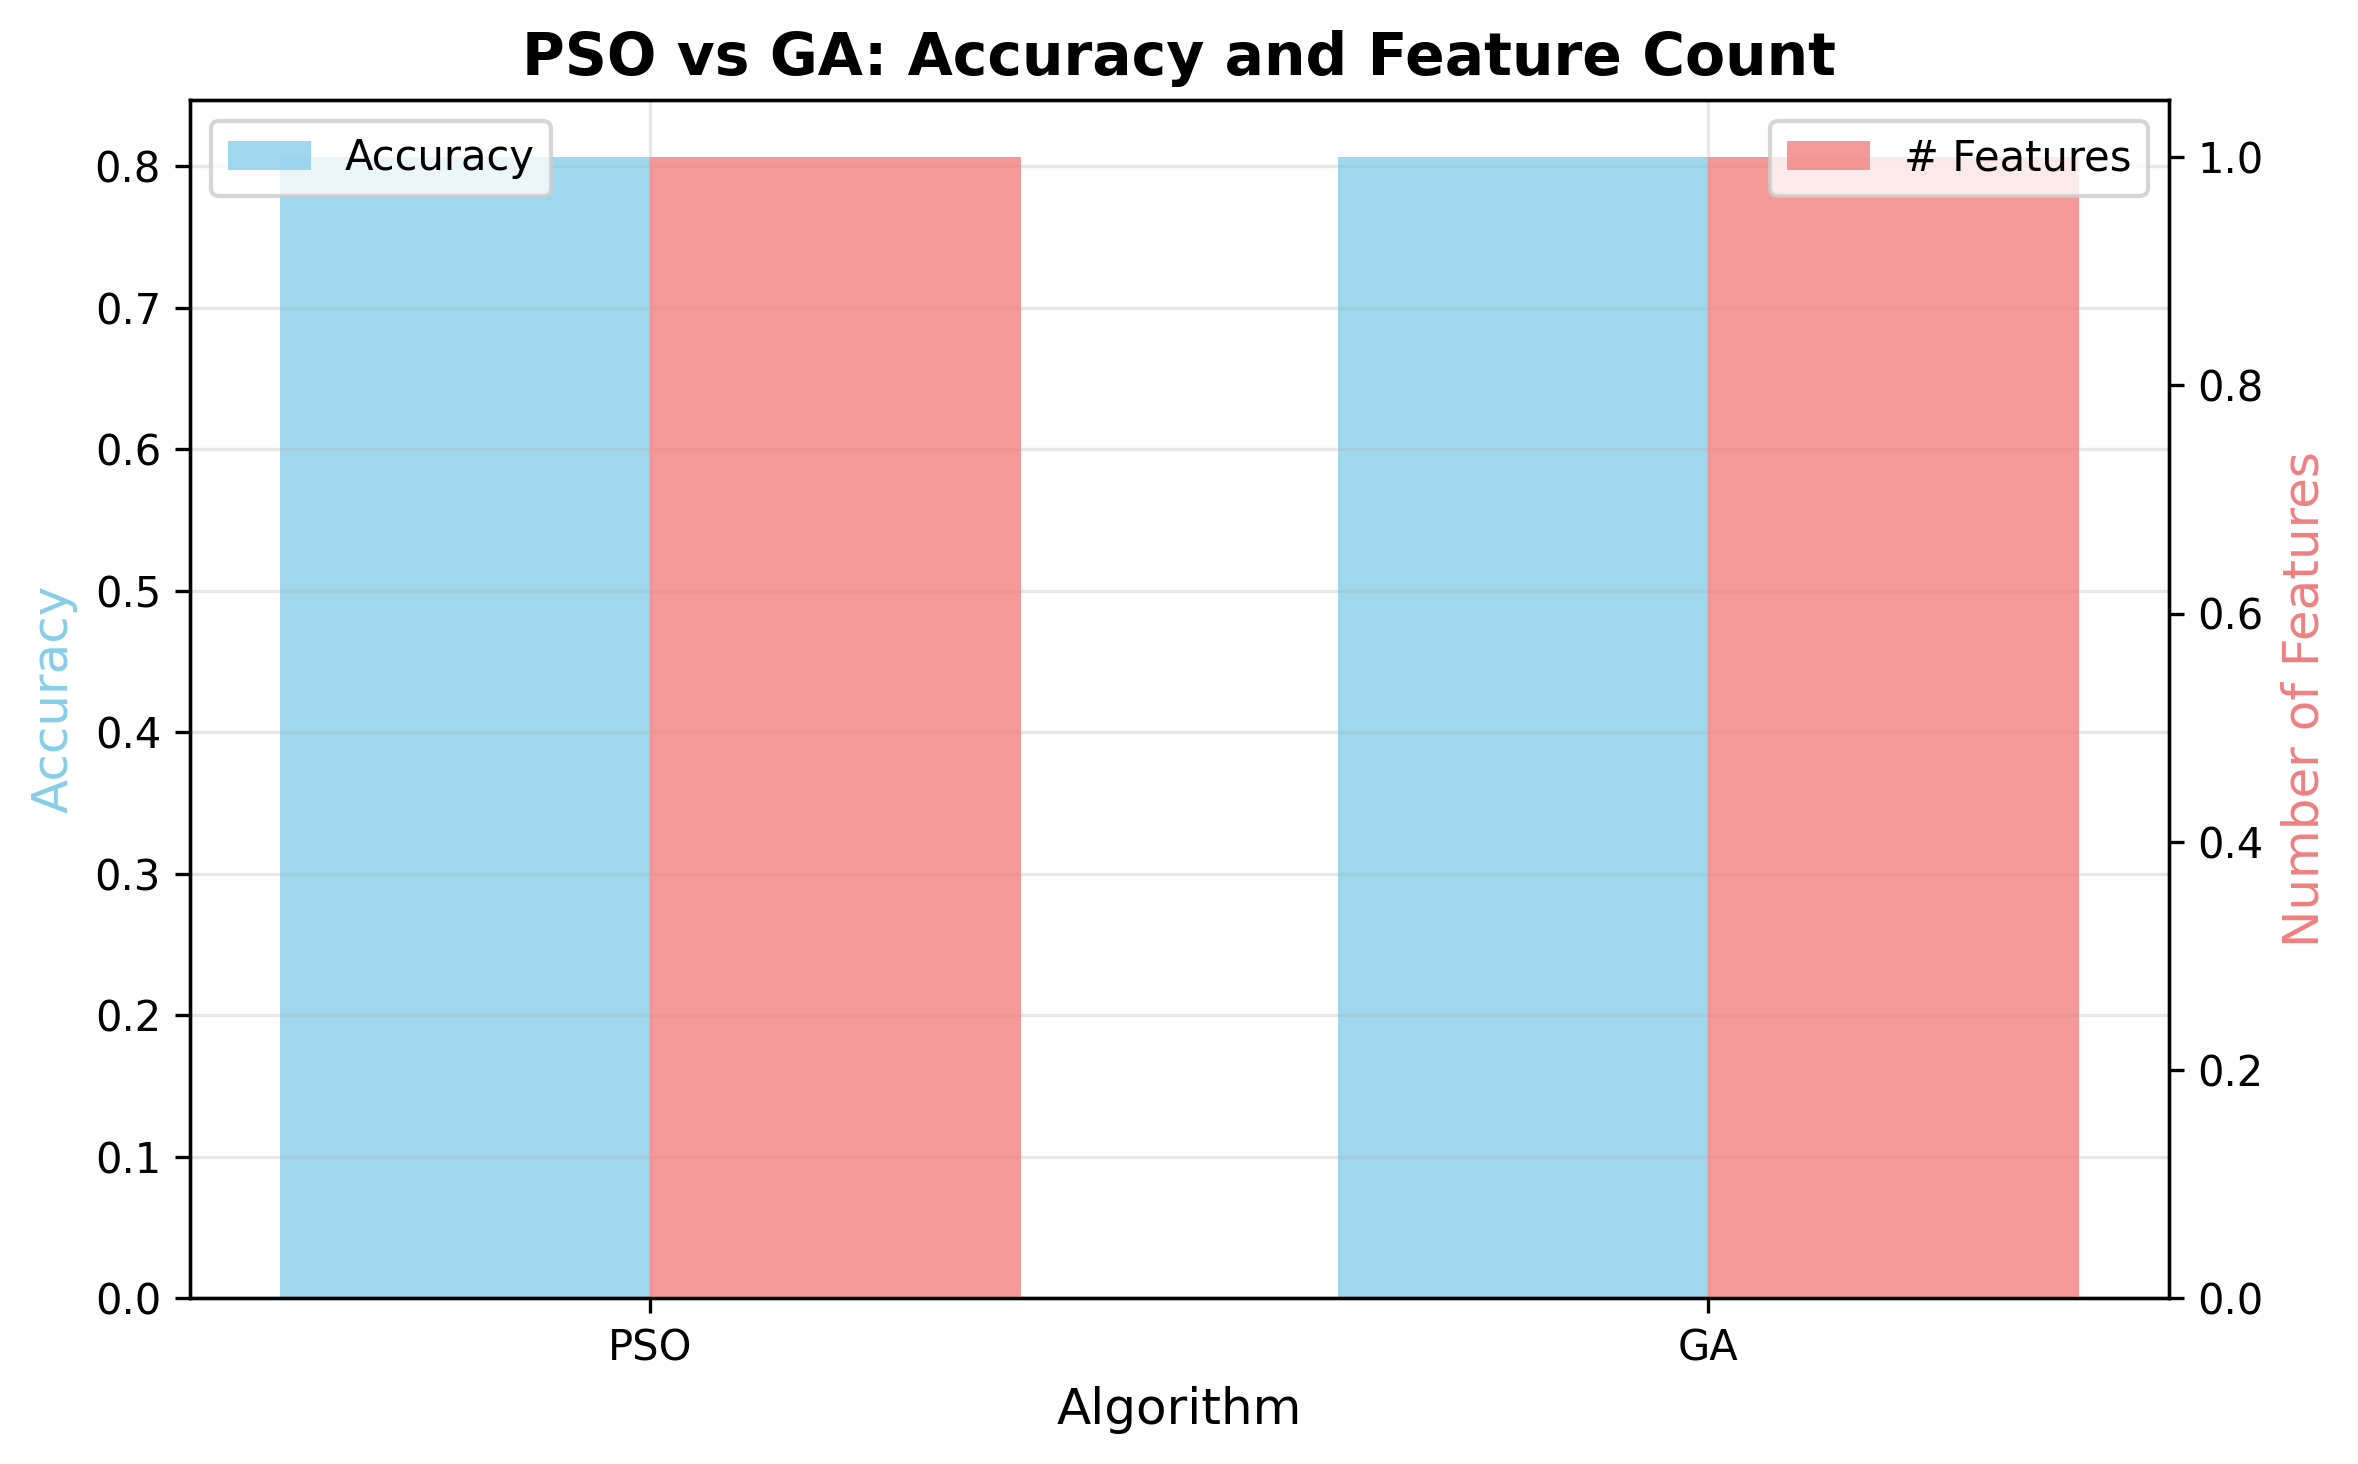
\includegraphics[width=0.9\textwidth]{img/question1_comparison.png}
    \caption{مقایسه عملکرد الگوریتم‌های PSO و GA شامل نمودار همگرایی، مقایسه دقت و تعداد ویژگی‌های انتخاب شده}
    \label{fig:q1_comparison}
\end{figure}

\subsubsection{تحلیل عملکرد و مقایسه جامع}

هر دو الگوریتم به دقت یکسان 0.8067 دست یافتند و هر دو ویژگی \lr{Credit\_History} را به عنوان مهم‌ترین ویژگی انتخاب کردند. این نتیجه مشترک نشان می‌دهد که تاریخچه اعتباری مهم‌ترین عامل در پیش‌بینی وضعیت وام است و کاهش ابعاد از 11 ویژگی به 1 ویژگی که معادل کاهش 90.9 درصدی است با حفظ دقت بالا امکان‌پذیر است. مدل تک‌ویژگی حاصل شده بسیار قابل تفسیر است و سادگی آن باعث می‌شود که برای استقرار در محیط عملیاتی مناسب باشد. همچنین این که هر دو الگوریتم به جواب یکسانی رسیدند نشان می‌دهد که جواب بهینه پایدار است و به الگوریتم خاصی بستگی ندارد.

مقایسه سرعت همگرایی نشان می‌دهد که الگوریتم PSO در تکرار 7 به جواب بهینه رسید در حالی که الگوریتم GA در نسل 3 به جواب بهینه رسید. بر این اساس به نظر می‌رسد GA سریع‌تر همگرا شده است اما این مقایسه کاملاً عادلانه نیست چون هر تکرار PSO شامل ارزیابی 50 ذره است و هر نسل GA شامل ارزیابی 50 فرد است اما محاسبات درونی این دو الگوریتم متفاوت است و نمی‌توان به طور مستقیم تعداد تکرارها را با تعداد نسل‌ها مقایسه کرد.

مقایسه پایداری نتایج نشان می‌دهد که الگوریتم PSO پس از رسیدن به جواب بهینه، نوسانات جزئی داشت و هزینه در محدوده 0.1626 تا 0.1992 تغییر کرد. در مقابل، الگوریتم GA پس از رسیدن به جواب بهینه، برازش بهترین فرد ثابت ماند اما برازش متوسط نوسان داشت که نشان‌دهنده اکتشاف مداوم فضای جستجو است. با این حال، هر دو الگوریتم جواب پایدار پیدا کردند و جواب بهینه در هر دو مورد حفظ شد.

مقایسه استراتژی جستجو نشان می‌دهد که الگوریتم PSO از جستجوی پیوسته در فضای ویژگی‌ها استفاده می‌کند و حرکت ذرات بر اساس سرعت و موقعیت انجام می‌شود. این استراتژی برای مسائل پیوسته و گسسته مناسب است. در مقابل، الگوریتم GA از جستجوی گسسته با عملگرهای ژنتیک استفاده می‌کند که شامل تقاطع و جهش برای ایجاد تنوع است. این استراتژی برای مسائل گسسته و ترکیبی مناسب است و در این مسئله خاص که انتخاب ویژگی یک مسئله گسسته است، عملکرد بهتری داشته است.

\textbf{مزایا و معایب}:
\begin{table}[h!]
\centering
\begin{tabular}{|p{3cm}|p{5cm}|p{5cm}|}
\hline
\textbf{معیار} & \textbf{PSO} & \textbf{GA} \\
\hline
سرعت همگرایی & متوسط (7 تکرار) & سریع (3 نسل) \\
\hline
پایداری & خوب & خوب \\
\hline
پیچیدگی پیاده‌سازی & متوسط & متوسط-بالا \\
\hline
پارامترهای تنظیم & 5 پارامتر اصلی & 4 پارامتر اصلی \\
\hline
قابلیت تفسیر & متوسط & متوسط \\
\hline
\end{tabular}
\caption{مقایسه الگوریتم‌های PSO و GA}
\label{tab:q1_comparison}
\end{table}

تحلیل نمودار همگرایی نشان می‌دهد که هر دو الگوریتم به سرعت به جواب بهینه نزدیک شدند. الگوریتم GA زودتر به جواب رسید اما PSO نیز به سرعت همگرا شد. پس از رسیدن به جواب بهینه، هر دو الگوریتم آن را حفظ کردند اما نوسانات در PSO بیشتر است که نشان‌دهنده اکتشاف مداوم فضای جستجو است.

نتیجه‌گیری کلی این است که هر دو الگوریتم عملکرد یکسانی داشتند و به جواب یکسانی رسیدند. الگوریتم GA کمی سریع‌تر همگرا شد اما انتخاب بین آن‌ها به عوامل دیگری مانند پیاده‌سازی، پارامترهای موجود و ترجیحات بستگی دارد. مهم‌ترین نتیجه این تحلیل این است که ویژگی \lr{Credit\_History} به تنهایی می‌تواند 80.67\% دقت داشته باشد که نشان‌دهنده اهمیت بالای این ویژگی است.

با این حال، مشکلات احتمالی وجود دارد که باید مورد توجه قرار گیرد. انتخاب تنها یک ویژگی ممکن است نشان‌دهنده این باشد که سایر ویژگی‌ها اطلاعات کمی دارند یا پارامتر $\alpha$ خیلی بالا است و اولویت بیشتری به دقت داده شده است. برای بررسی این موضوع می‌توان $\alpha$ را کاهش داد تا الگوریتم ویژگی‌های بیشتری را انتخاب کند و ببینیم آیا دقت بهبود می‌یابد. همچنین دقت 80.67\% ممکن است برای برخی کاربردها کافی نباشد و در این صورت می‌توان از روش‌های دیگر مانند \lr{Recursive Feature Elimination} یا \lr{Forward Selection} استفاده کرد.

\section{سوال ۲: خوشه‌بندی و کاهش ابعاد}\label{sec:q2}

\subsection{مقدمه}

در این بخش، خوشه‌بندی داده‌های مشتریان مرکز خرید با استفاده از سه الگوریتم مختلف انجام شده است: الگوریتم \lr{K-Means Clustering} که یک روش خوشه‌بندی مبتنی بر مرکز است، الگوریتم \lr{Agglomerative Hierarchical Clustering} که یک روش خوشه‌بندی سلسله‌مراتبی است، و الگوریتم \lr{DBSCAN} که یک روش خوشه‌بندی مبتنی بر چگالی است. هدف از این تحلیل، شناسایی الگوهای مشتریان و تقسیم آن‌ها به گروه‌های همگن برای استراتژی‌های بازاریابی هدفمند است.

\subsection{پیش‌پردازش داده}

داده‌های مشتریان مرکز خرید شامل 200 نمونه و 3 ویژگی عددی است که شامل سن مشتری (\lr{Age}) بر حسب سال، درآمد سالانه (\lr{Annual Income}) بر حسب هزار دلار، و امتیاز خرج کردن (\lr{Spending Score}) در محدوده 1 تا 100 می‌شود. برای آماده‌سازی داده‌ها، همه ویژگی‌ها با استفاده از \lr{StandardScaler} نرمال‌سازی شدند که بر اساس فرمول $z = \frac{x - \mu}{\sigma}$ عمل می‌کند. هدف از این نرمال‌سازی اطمینان از این است که همه ویژگی‌ها در مقیاس یکسان هستند که برای الگوریتم‌های مبتنی بر فاصله مانند K-Means و DBSCAN ضروری است. نکته مهم این است که تمام الگوریتم‌های خوشه‌بندی روی فضای اصلی 3 بعدی آموزش داده شدند و PCA تنها برای تجسم 2 بعدی استفاده شد.

\subsection{تحلیل مؤلفه اصلی (PCA)}

با استفاده از \lr{PCA} دو بعدی برای تجسم، نسبت واریانس توضیح داده شده برای بعد اول 0.4427 معادل 44.27\% و برای بعد دوم 0.3331 معادل 33.31\% است. واریانس تجمعی در 2 بعد برابر 0.7757 معادل 77.57\% است که نشان می‌دهد در مجموع 77.57\% از واریانس در 2 بعد حفظ شده است. این مقدار برای تجسم مناسب است اما 22.43\% اطلاعات از دست رفته است که باید در تفسیر نتایج در نظر گرفته شود.

مؤلفه اول ترکیبی از Age و Spending Score با وزن‌های متضاد است که وزن Age برابر 0.7064، وزن Annual Income برابر -0.0480 و وزن Spending Score برابر -0.7062 است. مؤلفه دوم عمدتاً Annual Income را نشان می‌دهد که وزن Age برابر 0.0301، وزن Annual Income برابر 0.9988 و وزن Spending Score برابر -0.0378 است. تفسیر این نتایج نشان می‌دهد که مؤلفه اول عمدتاً Age و Spending Score را جدا می‌کند که نشان‌دهنده همبستگی منفی بین این دو متغیر است. مؤلفه دوم عمدتاً Annual Income را نشان می‌دهد که نشان می‌دهد این متغیر مستقل از دو متغیر دیگر است.

\subsection{خوشه‌بندی K-Means}

الگوریتم \lr{K-Means} یک الگوریتم خوشه‌بندی مبتنی بر مرکز است که داده‌ها را به K خوشه تقسیم می‌کند. این الگوریتم با به حداقل رساندن مجموع مربعات فاصله نقاط از مرکز خوشه‌ها کار می‌کند.

مکانیزم الگوریتم به این صورت است که ابتدا K مرکز به صورت تصادفی انتخاب می‌شوند. سپس هر نقطه به نزدیک‌ترین مرکز تخصیص داده می‌شود و مراکز بر اساس میانگین نقاط تخصیص داده شده به‌روزرسانی می‌شوند. این فرآیند تا رسیدن به همگرایی تکرار می‌شود.

معیارهای ارزیابی شامل Inertia که مجموع مربعات فاصله نقاط از مرکز خوشه‌ها است و کمتر بهتر است، و Silhouette Score که معیار کیفیت خوشه‌بندی است و بیشتر بهتر است و در محدوده \lr{[-1, 1]} قرار دارد. Silhouette Score نزدیک به \lr{1} نشان می‌دهد که خوشه‌ها به خوبی جدا شده‌اند، نزدیک به \lr{0} نشان می‌دهد که خوشه‌ها همپوشانی دارند و نزدیک به \lr{-1} نشان می‌دهد که نقاط در خوشه‌های اشتباه قرار دارند.

\subsubsection{تحلیل جامع K از 2 تا 10}

با تست K از 2 تا 10، نتایج به شرح زیر است:

\begin{table}[h!]
\centering
\small
\begin{tabular}{|c|c|c|}
\hline
\textbf{K} & \textbf{Inertia} & \textbf{Silhouette Score} \\
\hline
\lr{2} & \lr{389.39} & \lr{0.3355} \\
\hline
\lr{3} & \lr{295.46} & \lr{0.3579} \\
\hline
\lr{4} & \lr{205.23} & \lr{0.4040} \\
\hline
\lr{5} & \lr{170.92} & \lr{0.4103} \\
\hline
\textbf{\lr{6}} & \textbf{\lr{151.57}} & \textbf{\lr{0.4274}} \\
\hline
\lr{7} & \lr{138.94} & \lr{0.4046} \\
\hline
\lr{8} & \lr{128.32} & \lr{0.3951} \\
\hline
\lr{9} & \lr{119.94} & \lr{0.3842} \\
\hline
\lr{10} & \lr{112.19} & \lr{0.3754} \\
\hline
\end{tabular}
\caption{نتایج K-Means برای K های مختلف}
\label{tab:kmeans_results}
\end{table}

تحلیل نتایج نشان می‌دهد که با \lr{K=2}، Silhouette برابر \lr{0.3355} است که پایین است و Inertia برابر \lr{389.39} است که بالا است. این نشان می‌دهد که خوشه‌ها خیلی بزرگ و ناهمگن هستند. با \lr{K=3}، Silhouette به \lr{0.3579} بهبود یافت و Inertia به \lr{295.46} کاهش یافت که بهبود نسبت به \lr{K=2} است اما هنوز بهینه نیست. با \lr{K=4}، Silhouette به \lr{0.4040} رسید که بهبود قابل توجهی است و Inertia به \lr{205.23} کاهش شدید یافت که نشان می‌دهد کیفیت خوشه‌بندی بهتر شده است. با \lr{K=5}، Silhouette به \lr{0.4103} رسید که بهترین تا اینجا بود و Inertia به \lr{170.92} کاهش یافت که نشان می‌دهد نزدیک به بهینه است.

با \lr{K=6}، Silhouette به \lr{0.4274} رسید که بهترین مقدار است و Inertia به \lr{151.57} کاهش یافت که نشان می‌دهد بهترین تعادل بین کیفیت و تعداد خوشه‌ها حاصل شده است. با \lr{K=7}، Silhouette به \lr{0.4046} کاهش یافت در حالی که Inertia به \lr{138.94} کاهش یافت. این نشان می‌دهد که با وجود کاهش Inertia، Silhouette کاهش یافته است که نشان می‌دهد خوشه‌ها بیش از حد تقسیم شده‌اند. با \lr{K=8} تا \lr{K=10}، Silhouette به تدریج کاهش می‌یابد در حالی که Inertia همچنان کاهش می‌یابد که طبیعی است اما خوشه‌ها بیش از حد تقسیم شده‌اند و کیفیت خوشه‌بندی کاهش یافته است.

\subsubsection{انتخاب K بهینه}

\textbf{K بهینه: \lr{6}} با امتیاز Silhouette برابر \lr{0.4274}

توجیه انتخاب \lr{K=6} بر اساس دو روش است. در روش Elbow، با افزایش K، Inertia کاهش می‌یابد اما نرخ کاهش در \lr{K=6} کند می‌شود که نشان می‌دهد این نقطه بهینه است. در روش Silhouette، \lr{K=6} بالاترین امتیاز Silhouette را دارد که نشان می‌دهد این مقدار بهترین کیفیت خوشه‌بندی را ایجاد می‌کند. \lr{K=6} تعادل خوبی بین کیفیت خوشه‌بندی و تعداد خوشه‌ها ایجاد می‌کند و \lr{6} خوشه برای استراتژی بازاریابی قابل مدیریت است.

با \lr{K=6}، داده‌ها به \lr{6} خوشه تقسیم شدند که هر کدام ویژگی‌های مشتریان خاصی را نشان می‌دهند. این خوشه‌ها می‌توانند برای استراتژی‌های بازاریابی هدفمند، پیشنهاد محصولات شخصی‌سازی شده و مدیریت روابط مشتری استفاده شوند.

با این حال، مشکلات احتمالی وجود دارد. Silhouette Score برابر \lr{0.4274} نشان می‌دهد که خوشه‌ها به خوبی جدا نشده‌اند. این مقدار در محدوده متوسط است (\lr{0.4-0.5}) که نشان می‌دهد داده‌ها ممکن است ساختار خوشه‌ای قوی نداشته باشند یا خوشه‌ها همپوشانی دارند. برای بهبود نتایج می‌توان از الگوریتم‌های دیگر مانند DBSCAN استفاده کرد که برای داده‌های با ساختار ضعیف مناسب‌تر است.

\subsection{خوشه‌بندی سلسله‌مراتبی تجمعی}

الگوریتم خوشه‌بندی سلسله‌مراتبی از پایین به بالا (\lr{bottom-up}) که با هر نقطه به عنوان یک خوشه شروع می‌کند و خوشه‌ها را بر اساس معیارهای پیوند (\lr{linkage}) ادغام می‌کند تا به تعداد خوشه‌های مطلوب برسد.

\textbf{مکانیزم الگوریتم}:
\begin{enumerate}
    \item شروع با N خوشه (هر نقطه یک خوشه)
    \item محاسبه فاصله بین همه جفت خوشه‌ها
    \item ادغام نزدیک‌ترین خوشه‌ها بر اساس معیار پیوند
    \item تکرار تا رسیدن به تعداد خوشه‌های مطلوب
    \item ایجاد درخت سلسله‌مراتبی (\lr{dendrogram})
\end{enumerate}

مزایای خوشه‌بندی سلسله‌مراتبی شامل این است که نیازی به تعیین تعداد خوشه‌ها از ابتدا نیست، ساختار سلسله‌مراتبی را نشان می‌دهد که می‌توان در سطوح مختلف خوشه‌بندی را مشاهده کرد و برای داده‌های کوچک تا متوسط مناسب است.

\subsubsection{مقایسه روش‌های پیوند}

چهار روش پیوند مختلف تست شدند:

\begin{table}[h!]
\centering
\small
\begin{tabular}{|c|c|c|}
\hline
\textbf{روش پیوند} & \textbf{Silhouette Score} & \textbf{توضیحات} \\
\hline
Single & \lr{-0.0428} & فاصله بین نزدیک‌ترین نقاط \\
\hline
Complete & \lr{0.3746} & فاصله بین دورترین نقاط \\
\hline
Average & \lr{0.3896} & میانگین فاصله بین نقاط \\
\hline
\textbf{Ward} & \textbf{\lr{0.4201}} & \textbf{حداقل واریانس درون خوشه‌ای} \\
\hline
\end{tabular}
\caption{مقایسه روش‌های پیوند در خوشه‌بندی سلسله‌مراتبی}
\label{tab:linkage_comparison}
\end{table}

تحلیل هر روش نشان می‌دهد که Single Linkage با Silhouette برابر \lr{-0.0428} بدترین عملکرد را داشت. این روش از فاصله بین نزدیک‌ترین نقاط دو خوشه استفاده می‌کند که مشکل ایجاد خوشه‌های زنجیره‌ای (\lr{chain clusters}) را دارد و حساس به داده‌های پرت است و برای این داده مناسب نیست.

Complete Linkage با Silhouette برابر \lr{0.3746} عملکرد متوسطی داشت. این روش از فاصله بین دورترین نقاط دو خوشه استفاده می‌کند که مزیت آن تولید خوشه‌های فشرده و کروی است و مقاوم به داده‌های پرت است اما عملکرد متوسطی دارد.

Average Linkage با Silhouette برابر \lr{0.3896} عملکرد خوبی داشت. این روش از میانگین فاصله بین همه جفت نقاط استفاده می‌کند که تعادل بین Single و Complete ایجاد می‌کند و عملکرد خوب اما نه بهینه دارد.

Ward Linkage با Silhouette برابر \lr{0.4201} بهترین عملکرد را داشت. این روش با حداقل کردن افزایش واریانس درون خوشه‌ای پس از ادغام کار می‌کند که با فرمول $d(u,v) = \sqrt{\frac{|v|+|s|}{T}d(v,s)^2 + \frac{|v|+|t|}{T}d(v,t)^2 - \frac{|v|}{T}d(s,t)^2}$ محاسبه می‌شود. مزایای این روش شامل تولید خوشه‌های فشرده و کروی، مناسب بودن برای داده‌های با ساختار کروی و عملکرد بهتر نسبت به سایر روش‌ها است.

\subsubsection{بهترین روش پیوند}

\textbf{روش Ward} با امتیاز Silhouette برابر 0.4201 بهترین عملکرد را داشت.

توجیه انتخاب Ward شامل این است که این روش بالاترین امتیاز Silhouette در بین همه روش‌ها را دارد، واریانس درون خوشه‌ای را به حداقل می‌رساند و خوشه‌های فشرده و کروی تولید می‌کند. این روش برای داده‌های با ساختار کروی (مانند K-Means) مناسب است و مقاوم به داده‌های پرت است.

مقایسه با K-Means نشان می‌دهد که K-Means با \lr{K=6} و Silhouette برابر \lr{0.4274} کمی بهتر عمل کرد اما تفاوت ناچیز است و Agglomerative با Ward و \lr{K=6} و Silhouette برابر \lr{0.4201} عملکرد مشابهی داشت. هر دو روش برای داده‌های کروی مناسب هستند.

ساختار سلسله‌مراتبی این الگوریتم به این معناست که می‌توان در سطوح مختلف خوشه‌بندی را مشاهده کرد. برای مثال می‌توان \lr{2} خوشه اصلی داشت که هر کدام به زیرخوشه‌ها تقسیم می‌شوند که این ساختار برای استراتژی‌های بازاریابی چندسطحی مفید است.

محدودیت‌های این الگوریتم شامل پیچیدگی محاسباتی \lr{$O(n^3)$} است که برای داده‌های بزرگ کند است و نیاز به ذخیره ماتریس فاصله دارد که برای داده‌های بزرگ (بیش از \lr{10000} نمونه) مناسب نیست.

\subsection{خوشه‌بندی DBSCAN}

\lr{DBSCAN} (\lr{Density-Based Spatial Clustering of Applications with Noise}) یک الگوریتم خوشه‌بندی مبتنی بر چگالی است که می‌تواند خوشه‌های با شکل دلخواه را شناسایی کند و به طور طبیعی نقاط نویز را تشخیص دهد.

\textbf{مکانیزم الگوریتم}:
\begin{enumerate}
    \item تعریف همسایگی: نقاط در فاصله \lr{eps} از یک نقطه
    \item نقطه هسته (\lr{core point}): نقطه‌ای که حداقل \lr{min\_samples} همسایه دارد
    \item نقطه مرزی (\lr{border point}): نقطه‌ای که در همسایگی یک نقطه هسته است اما خودش هسته نیست
    \item نقطه نویز (\lr{noise point}): نقطه‌ای که نه هسته است و نه مرزی
    \item تشکیل خوشه: همه نقاط هسته و مرزی متصل به هم یک خوشه را تشکیل می‌دهند
\end{enumerate}

مزایای DBSCAN شامل این است که نیازی به تعیین تعداد خوشه‌ها از ابتدا نیست، می‌تواند خوشه‌های با شکل دلخواه را شناسایی کند، به طور طبیعی نقاط نویز را تشخیص می‌دهد و مقاوم به داده‌های پرت است.

محدودیت‌های DBSCAN شامل حساسیت به پارامترهای \lr{eps} و \lr{min\_samples} است که نیاز به تنظیم دقیق دارد. این الگوریتم برای داده‌های با چگالی متفاوت مشکل دارد و برای داده‌های با ابعاد بالا عملکرد ضعیفی دارد که یکی از محدودیت‌های مهم آن است.

\subsubsection{جستجوی شبکه پارامترها}

برای یافتن بهترین پارامترها، جستجوی شبکه (\lr{grid search}) انجام شد:

محدوده پارامترها شامل \lr{eps} با مقادیر \lr{[0.2, 0.4, 0.6, 0.8, 1.0]} که \lr{5} مقدار است و \lr{min\_samples} با مقادیر \lr{[3, 5, 10]} که \lr{3} مقدار است. تعداد کل پیکربندی‌ها برابر \lr{$5 \times 3 = 15$} است که همه آن‌ها مورد آزمایش قرار گرفتند.

تحلیل حساسیت پارامترها نشان می‌دهد که با \lr{eps} کوچک (\lr{0.2})، همسایگی کوچک است که منجر به خوشه‌های زیاد و کوچک می‌شود و نقاط نویز زیاد (حدود \lr{80\%}) ایجاد می‌کند که باعث Silhouette پایین می‌شود. با \lr{eps} متوسط (\lr{0.4-0.6})، همسایگی متوسط است که تعادل بین تعداد خوشه‌ها و نویز ایجاد می‌کند و عملکرد بهتری دارد. با \lr{eps} بزرگ (\lr{0.8-1.0})، همسایگی بزرگ است که منجر به خوشه‌های کم و بزرگ می‌شود و ممکن است همه نقاط در یک خوشه قرار گیرند که باعث از دست دادن ساختار خوشه‌ای می‌شود.

با \lr{min\_samples} کوچک (\lr{3})، نیاز به همسایگان کم است که منجر به خوشه‌های بیشتر می‌شود اما ممکن است نویز را به عنوان خوشه تشخیص دهد. با \lr{min\_samples} متوسط (\lr{5})، تعادل مناسبی ایجاد می‌شود و عملکرد خوبی دارد. با \lr{min\_samples} بزرگ (\lr{10})، نیاز به همسایگان بیشتر است که منجر به خوشه‌های محکم‌تر و نویز بیشتر می‌شود و برای داده‌های با چگالی بالا مناسب است.

\subsubsection{بهترین پیکربندی DBSCAN}

پارامترهای بهینه شامل \lr{eps} برابر \lr{0.6}، \lr{min\_samples} برابر \lr{10}، تعداد خوشه‌ها برابر \lr{4}، تعداد نقاط نویز برابر \lr{66} معادل \lr{33\%} و امتیاز Silhouette برابر \lr{0.5296} است که بهترین در بین همه الگوریتم‌ها است.

توجیه انتخاب این پارامترها به این صورت است. با \lr{eps=0.6}، تعادل خوبی بین شناسایی خوشه‌ها و تشخیص نویز ایجاد می‌شود که نه خیلی کوچک است (که خوشه‌های زیاد ایجاد می‌کند) و نه خیلی بزرگ است (که همه را در یک خوشه قرار می‌دهد). با \lr{min\_samples=10}، نیاز به حداقل \lr{10} همسایه برای نقطه هسته است که خوشه‌های محکم و فشرده ایجاد می‌کند و نقاط پرت را به عنوان نویز تشخیص می‌دهد. با \lr{4} خوشه، تعداد مناسب برای تفسیر است و هر خوشه گروه مشخصی از مشتریان را نشان می‌دهد. با \lr{33\%} نویز، این مقدار ممکن است بالا به نظر برسد اما نشان می‌دهد که \lr{33\%} از مشتریان الگوی مشخصی ندارند که می‌تواند برای استراتژی بازاریابی مفید باشد.

\textbf{مقایسه با سایر الگوریتم‌ها}:
\begin{table}[h!]
\centering
\small
\begin{tabular}{|c|c|c|}
\hline
\textbf{الگوریتم} & \textbf{Silhouette Score} & \textbf{تعداد خوشه‌ها} \\
\hline
K-Means (K=\lr{6}) & \lr{0.4274} & \lr{6} \\
\hline
Agglomerative (Ward) & \lr{0.4201} & \lr{6} \\
\hline
\textbf{DBSCAN} & \textbf{\lr{0.5296}} & \textbf{\lr{4}} \\
\hline
\end{tabular}
\caption{مقایسه عملکرد الگوریتم‌های خوشه‌بندی}
\label{tab:clustering_comparison}
\end{table}

دلایل عملکرد بهتر DBSCAN شامل چند عامل است. Silhouette Score بالاتر برابر \lr{0.5296} نشان می‌دهد که خوشه‌ها به خوبی جدا شده‌اند. DBSCAN به طور طبیعی نقاط نویز را تشخیص داد که یکی از مزایای مهم این الگوریتم است. این الگوریتم می‌تواند خوشه‌های غیرکروی را شناسایی کند که برای داده‌های با ساختار پیچیده مناسب است. همچنین نیازی به تعیین تعداد خوشه‌ها از ابتدا نیست که یکی از مزایای مهم این الگوریتم است.

با \lr{4} خوشه و \lr{66} نقطه نویز، می‌توان مشتریان را به گروه‌های مختلف تقسیم کرد. خوشه‌های \lr{1-4} گروه‌های اصلی مشتریان با الگوهای مشخص را نشان می‌دهند و نقاط نویز مشتریانی هستند که الگوی مشخصی ندارند و نیاز به تحلیل جداگانه دارند.

مشکلات احتمالی شامل این است که \lr{33\%} نویز ممکن است بالا باشد. این می‌تواند نشان دهد که داده‌ها ساختار خوشه‌ای قوی ندارند یا پارامترها نیاز به تنظیم دارند. برای بهبود نتایج می‌توان \lr{eps} را کمی افزایش داد یا \lr{min\_samples} را کاهش داد اما با توجه به Silhouette Score بالا، پیکربندی فعلی مناسب است و نیازی به تغییر نیست.

\subsection{تصاویر خوشه‌بندی}

\begin{figure}[h!]
    \centering
    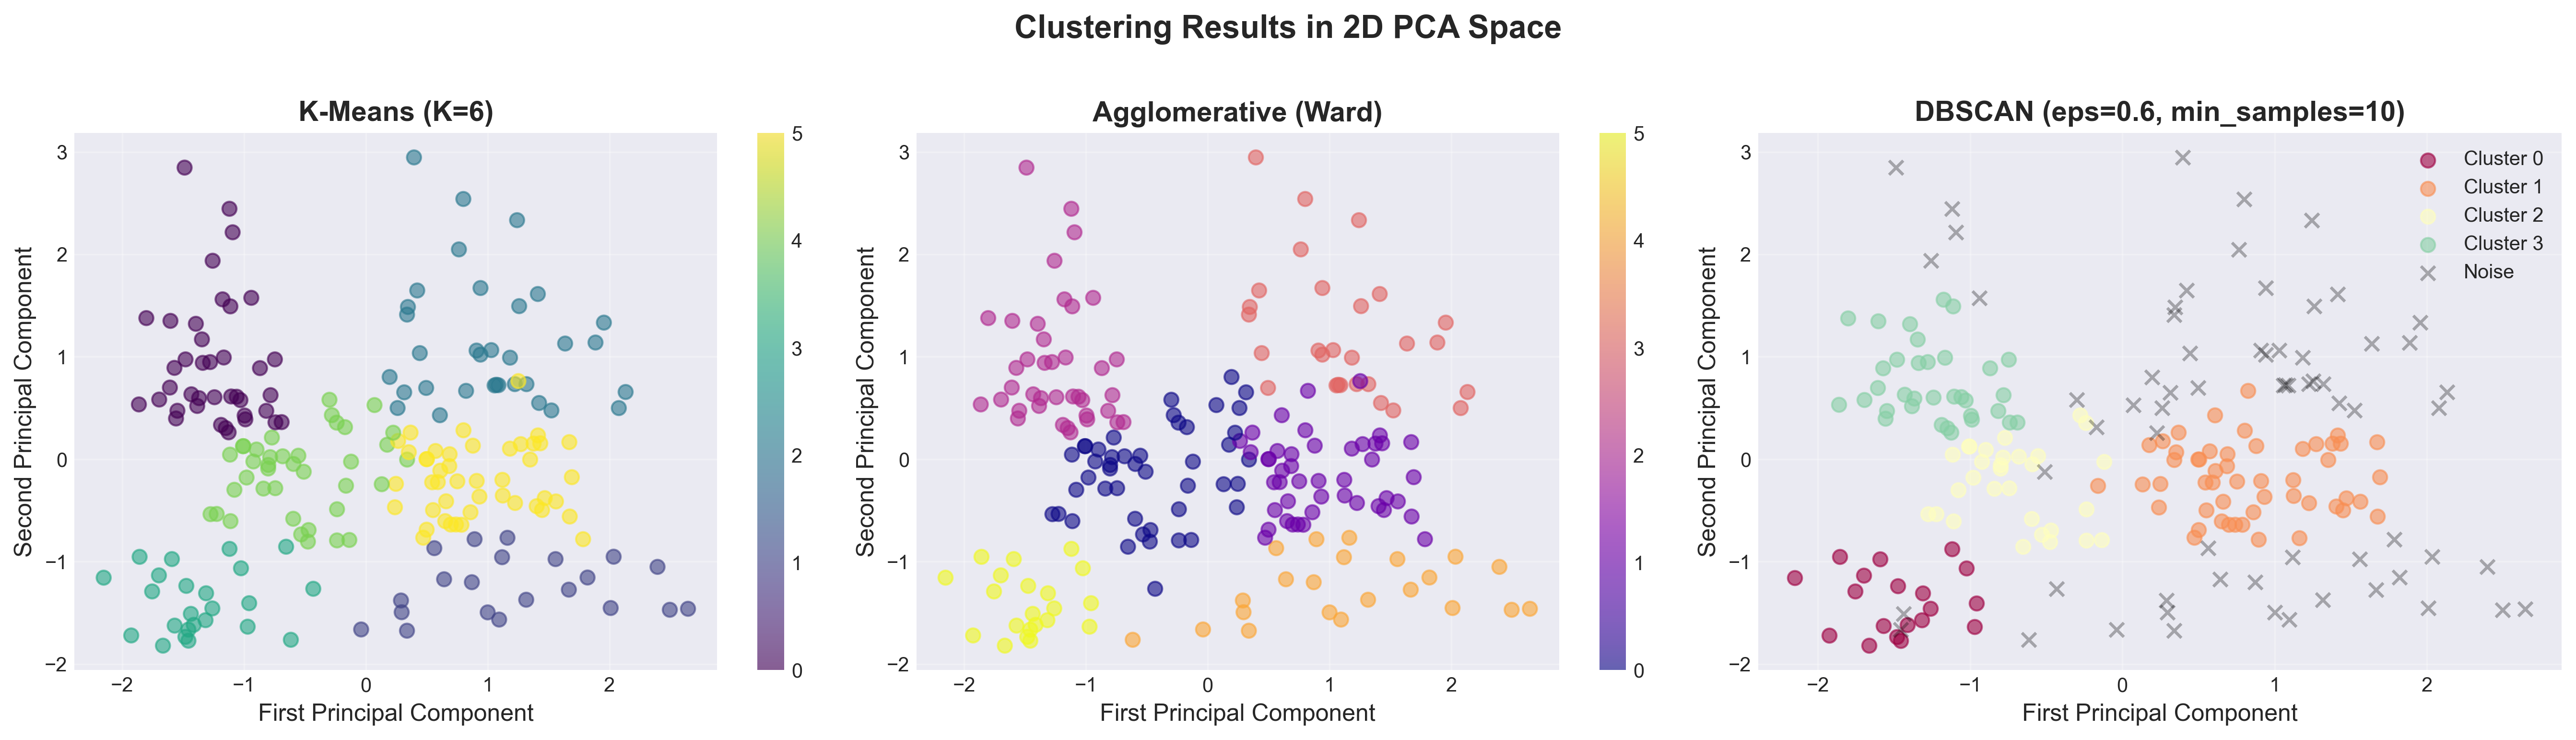
\includegraphics[width=0.9\textwidth]{img/question2_clustering_visualization.png}
    \caption{نمایش بصری خوشه‌بندی‌های مختلف در فضای دو بعدی PCA}
    \label{fig:q2_visualization}
\end{figure}

تحلیل نمودار نمایش بصری خوشه‌بندی‌ها در فضای دو بعدی PCA نشان می‌دهد که هر سه الگوریتم خوشه‌بندی ساختارهای متفاوتی را در داده‌ها شناسایی کرده‌اند. در نمودار K-Means با \lr{K=6}، می‌توان مشاهده کرد که خوشه‌ها به صورت کروی و فشرده در فضای دو بعدی توزیع شده‌اند. مراکز خوشه‌ها به خوبی از هم جدا شده‌اند که نشان می‌دهد الگوریتم توانسته است گروه‌های متمایزی از مشتریان را شناسایی کند. با این حال، برخی از خوشه‌ها همپوشانی دارند که با مقدار Silhouette Score برابر \lr{0.4274} مطابقت دارد.

در نمودار Agglomerative با Ward Linkage و \lr{K=6}، ساختار خوشه‌بندی مشابه K-Means است اما تفاوت‌های جزئی وجود دارد. خوشه‌ها در این روش نیز کروی هستند که با ماهیت Ward Linkage که واریانس درون خوشه‌ای را به حداقل می‌رساند، سازگار است. این روش خوشه‌های فشرده‌تری ایجاد کرده است که نشان می‌دهد برای داده‌های با ساختار کروی مناسب است.

در نمودار DBSCAN با \lr{eps=0.6} و \lr{min\_samples=10}، ساختار خوشه‌بندی کاملاً متفاوت است. این الگوریتم \lr{4} خوشه اصلی شناسایی کرده است و \lr{66} نقطه (\lr{33\%}) را به عنوان نویز تشخیص داده است که با رنگ متفاوت نمایش داده شده‌اند. خوشه‌های شناسایی شده توسط DBSCAN شکل غیرکروی دارند که یکی از مزایای مهم این الگوریتم است. نقاط نویز عمدتاً در مناطق با چگالی پایین قرار دارند که نشان می‌دهد این الگوریتم به خوبی مشتریانی را که الگوی مشخصی ندارند شناسایی کرده است.

مقایسه سه روش نشان می‌دهد که K-Means و Agglomerative خوشه‌های مشابهی ایجاد کرده‌اند که با ساختار کروی داده‌ها سازگار است. در مقابل، DBSCAN خوشه‌های متفاوتی شناسایی کرده است که نشان می‌دهد این الگوریتم ساختار پیچیده‌تری در داده‌ها کشف کرده است. این تفاوت با امتیاز Silhouette بالاتر DBSCAN (\lr{0.5296}) در مقایسه با دو روش دیگر مطابقت دارد.

\subsubsection{تحلیل معیارهای خوشه‌بندی}

در این بخش، چهار نمودار مختلف برای تحلیل جامع عملکرد الگوریتم‌های خوشه‌بندی ارائه شده است. هر نمودار به صورت جداگانه نمایش داده شده و تحلیل دقیقی از آن ارائه می‌شود.

\subsubsection{نمودار Inertia و Silhouette Score برای K-Means}

\begin{figure}[h!]
    \centering
    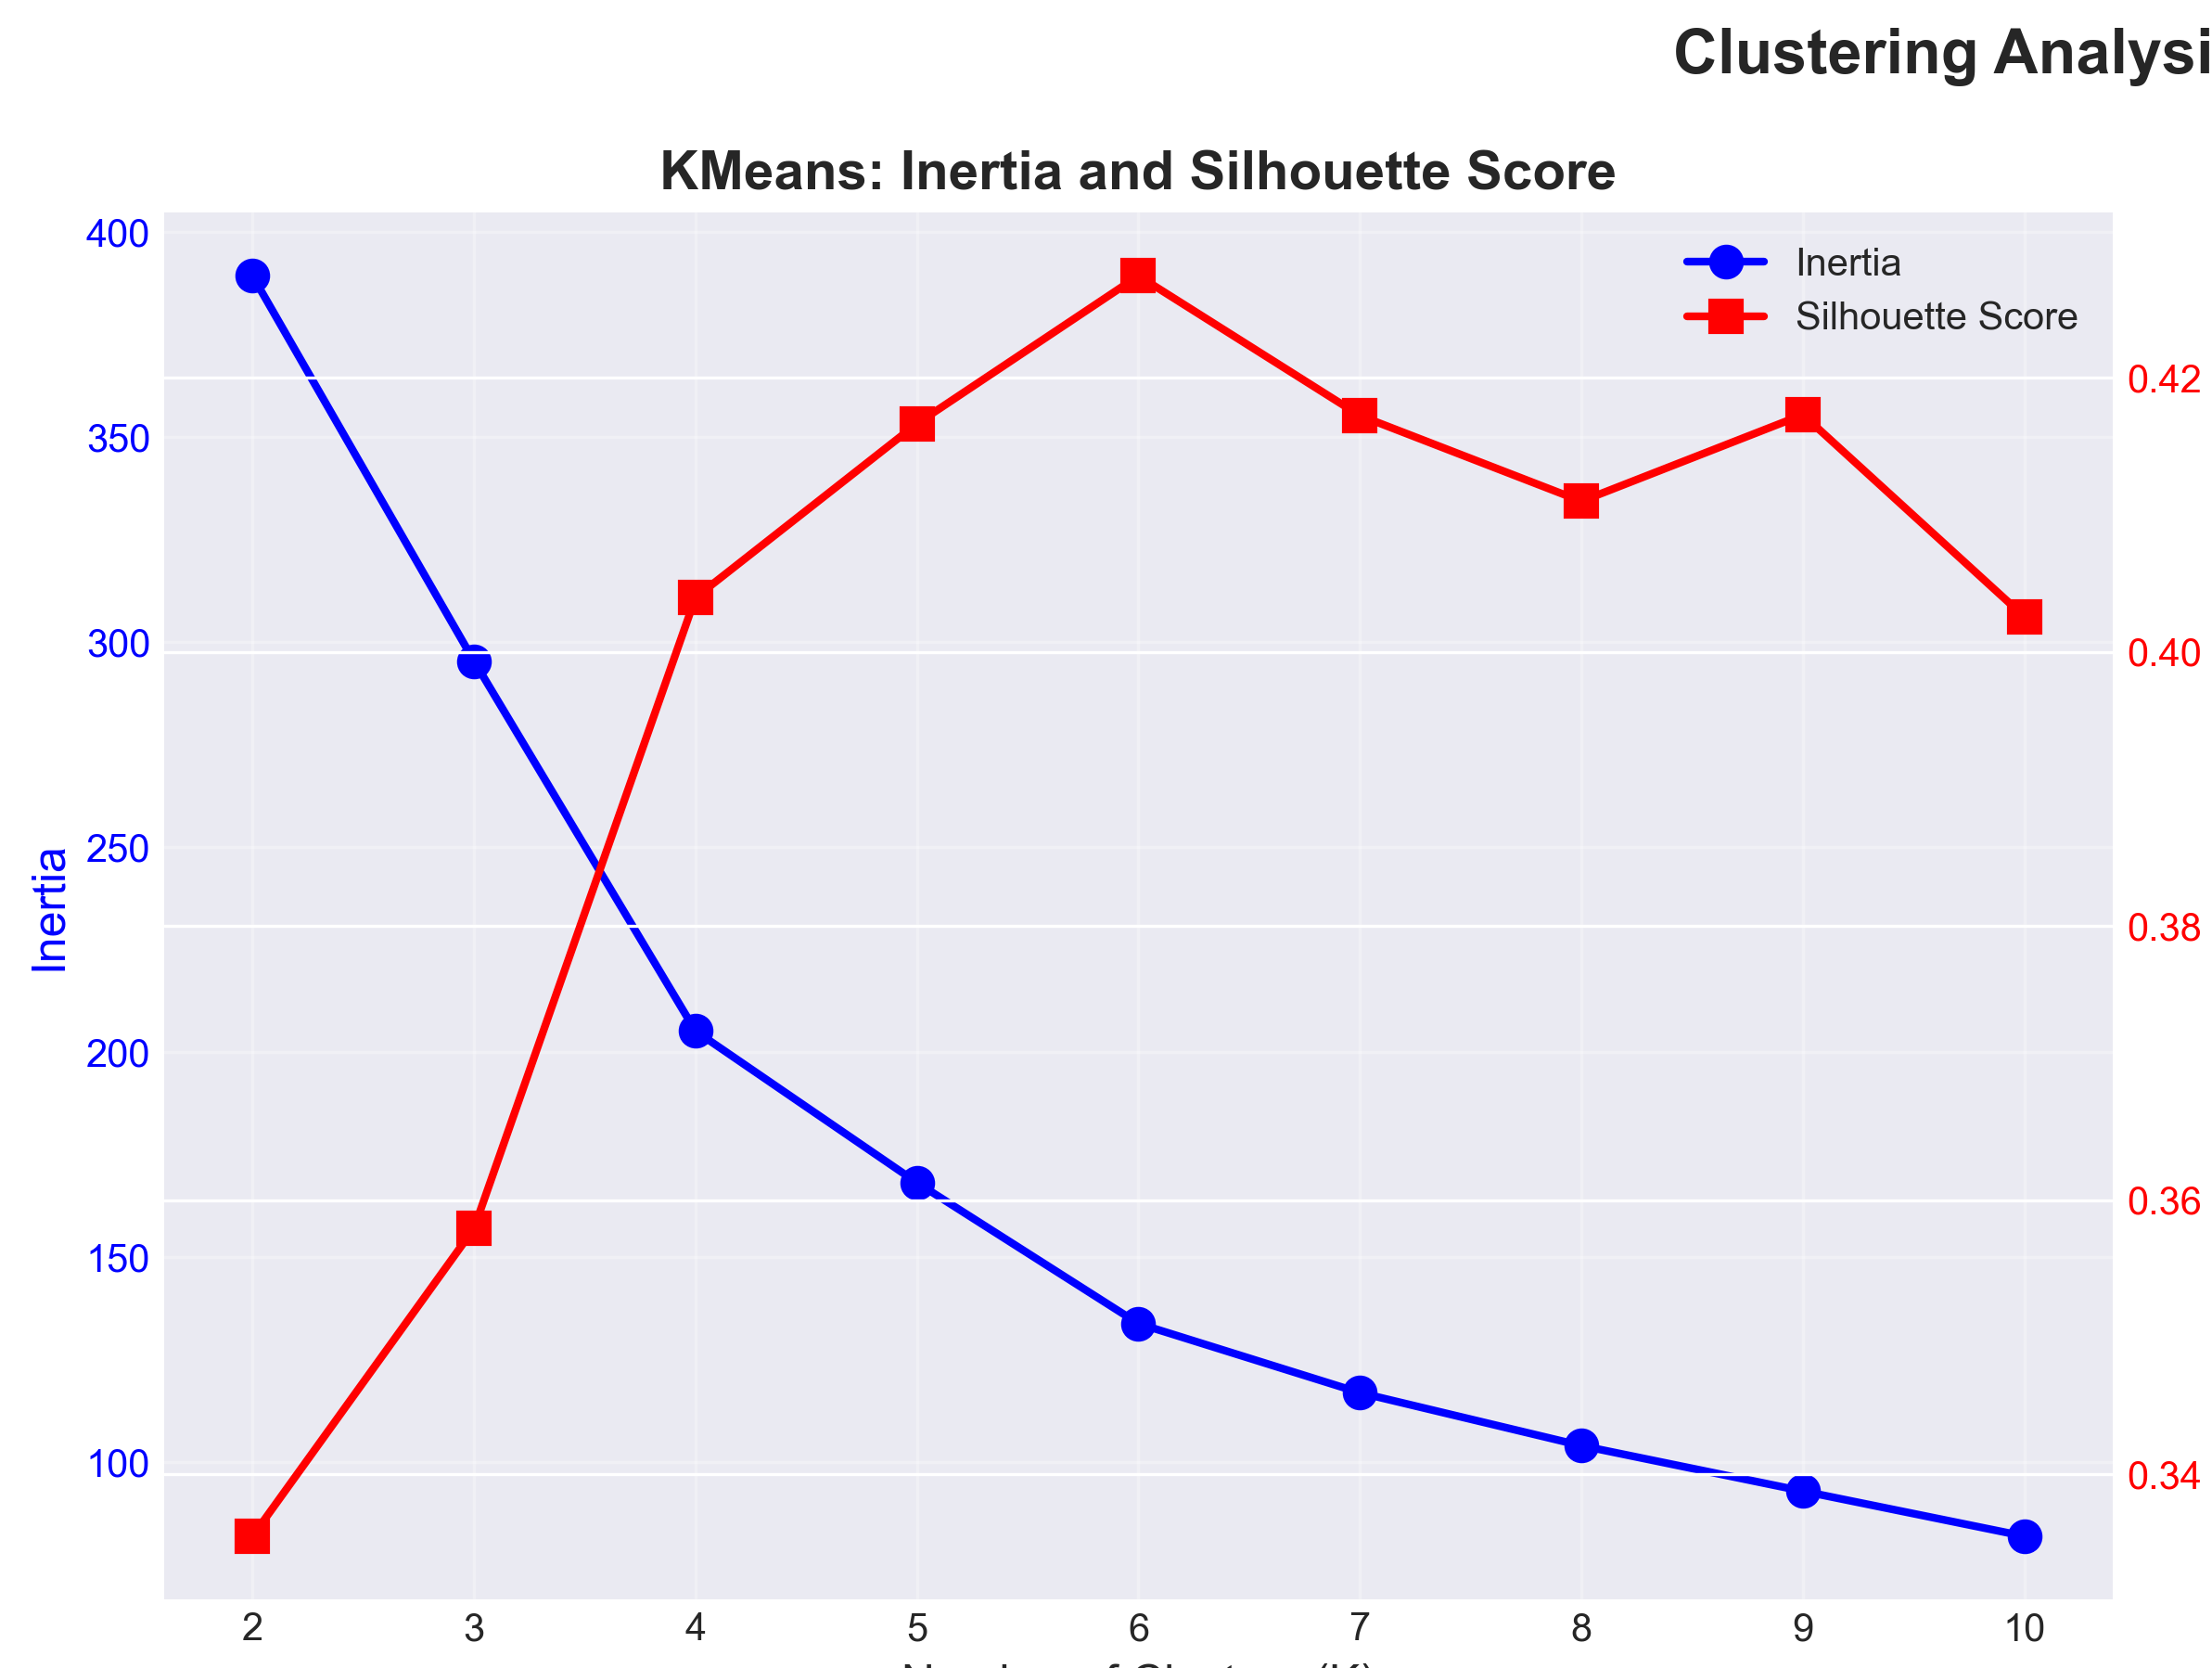
\includegraphics[width=0.8\textwidth]{img/question2_kmeans_inertia_silhouette.png}
    \caption{نمودار Inertia و Silhouette Score برای K-Means با تعداد خوشه‌های مختلف از \lr{K=2} تا \lr{K=10}}
    \label{fig:kmeans_inertia_silhouette}
\end{figure}

در شکل \ref{fig:kmeans_inertia_silhouette}، نمودار Inertia و Silhouette Score برای الگوریتم K-Means با تعداد خوشه‌های مختلف از \lr{K=2} تا \lr{K=10} نمایش داده شده است. این نمودار برای تعیین تعداد بهینه خوشه‌ها استفاده می‌شود.

\textbf{تحلیل Inertia}: با افزایش K، Inertia به طور مداوم کاهش می‌یابد که طبیعی است چون با افزایش تعداد خوشه‌ها، فاصله نقاط از مراکز کاهش می‌یابد. از حدود \lr{390} در \lr{K=2} به حدود \lr{80} در \lr{K=10} می‌رسد. یک نقطه "آرنج" (elbow) در حدود \lr{K=4} یا \lr{K=5} مشاهده می‌شود که نشان‌دهنده کاهش سرعت افت Inertia است. این نقطه نشان می‌دهد که افزایش بیشتر K بهبود قابل توجهی در کیفیت خوشه‌بندی ایجاد نمی‌کند.

\textbf{تحلیل Silhouette Score}: Silhouette Score از حدود \lr{0.335} در \lr{K=2} شروع شده، در \lr{K=6} به اوج خود (حدود \lr{0.427}) می‌رسد و سپس تا \lr{K=10} کمی کاهش می‌یابد (حدود \lr{0.400}). این نشان می‌دهد که \lr{K=6} تعداد بهینه خوشه‌ها است چون بالاترین Silhouette Score را دارد.

\textbf{نتیجه‌گیری}: با توجه به اوج Silhouette Score در \lr{K=6} و نقطه آرنج در Inertia در حدود \lr{K=4} یا \lr{K=5}، \lr{K=6} به عنوان تعداد بهینه خوشه‌ها انتخاب شد که تعادل خوبی بین کیفیت خوشه‌بندی و پیچیدگی مدل ایجاد می‌کند.

\subsubsection{مقایسه Silhouette Score برای روش‌های پیوند Agglomerative}

\begin{figure}[h!]
    \centering
    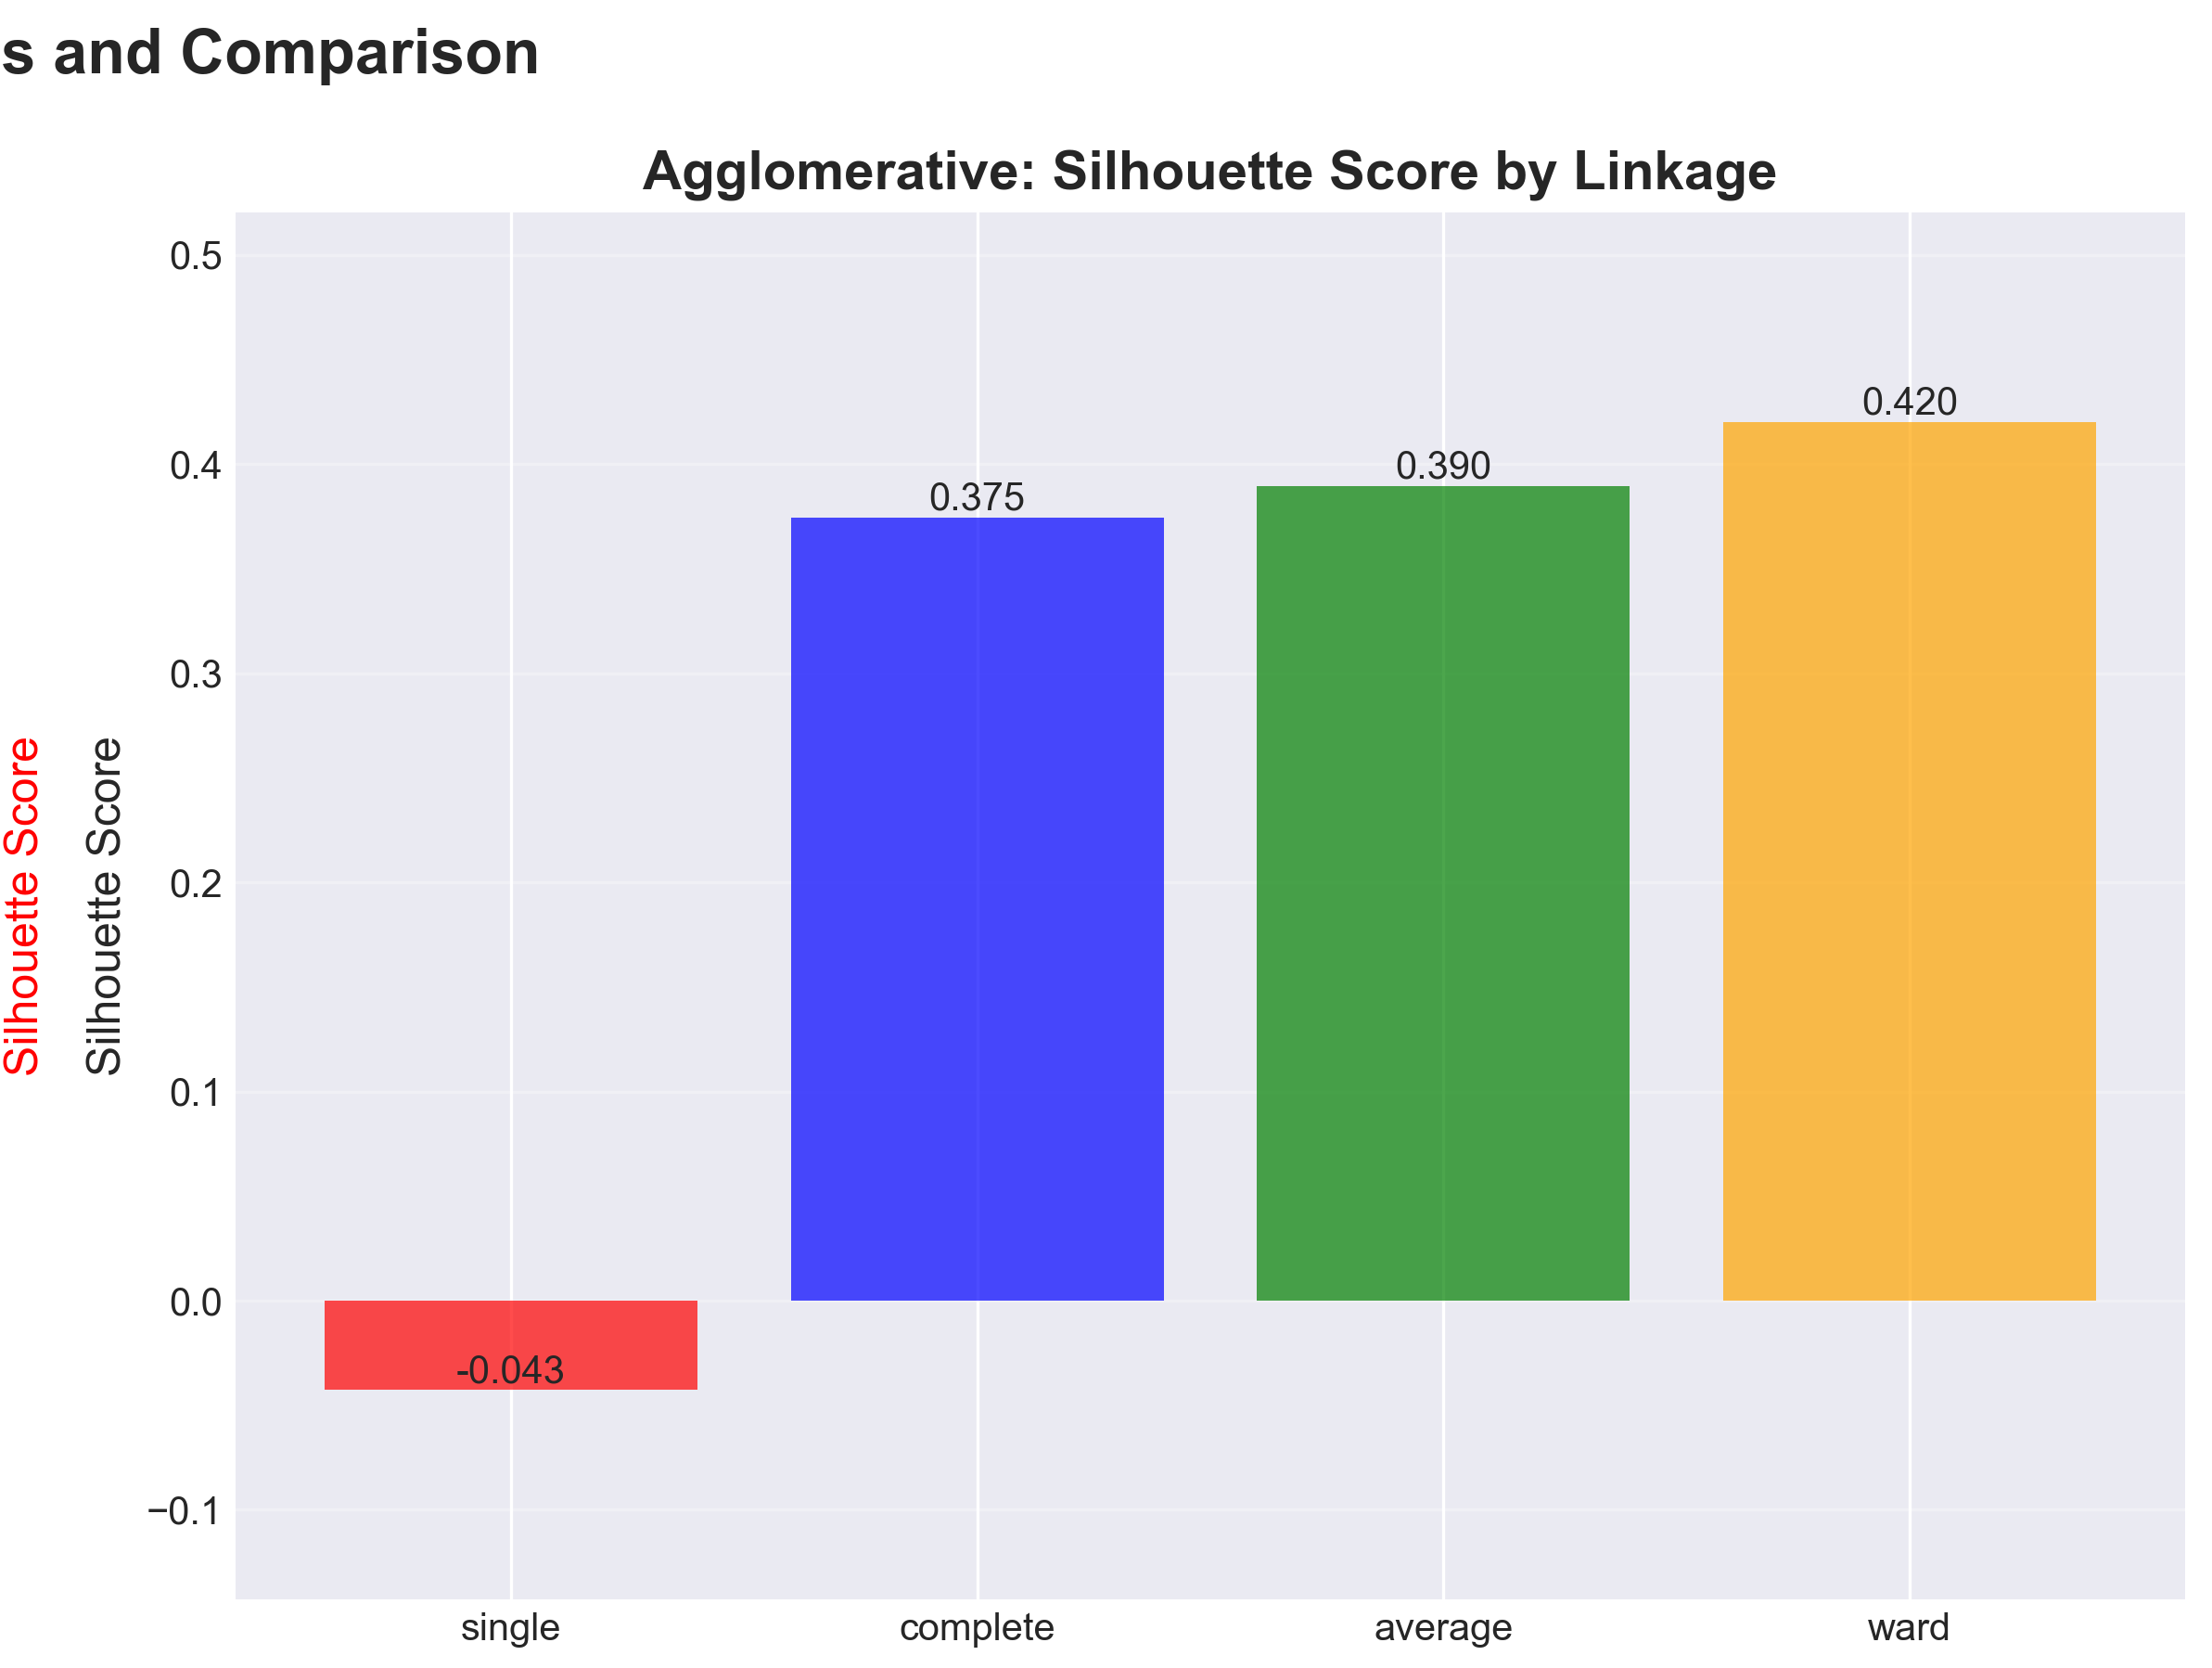
\includegraphics[width=0.8\textwidth]{img/question2_agglomerative_linkage.png}
    \caption{مقایسه Silhouette Score برای چهار روش پیوند مختلف در الگوریتم Agglomerative Clustering}
    \label{fig:agglomerative_linkage_comparison}
\end{figure}

در شکل \ref{fig:agglomerative_linkage_comparison}، مقایسه Silhouette Score برای چهار روش پیوند مختلف در الگوریتم Agglomerative Clustering نمایش داده شده است.

\textbf{نتایج روش‌های پیوند}: روش \lr{single} با امتیاز \lr{-0.043} عملکرد بسیار ضعیفی دارد و حتی منفی است که نشان می‌دهد این روش برای این داده‌ها مناسب نیست. روش \lr{complete} با امتیاز \lr{0.375} عملکرد متوسطی دارد. روش \lr{average} با امتیاز \lr{0.399} عملکرد بهتری دارد. روش \lr{ward} با امتیاز \lr{0.420} بهترین عملکرد را دارد و بالاترین Silhouette Score را در بین همه روش‌های Agglomerative به دست آورده است.

\textbf{تحلیل عملکرد Ward Linkage}: روش Ward Linkage که واریانس درون خوشه‌ای را به حداقل می‌رساند، برای داده‌های با ساختار کروی مناسب است. این روش خوشه‌های فشرده‌تری ایجاد می‌کند که با ساختار داده‌های مشتریان مرکز خرید سازگار است.

\textbf{نتیجه‌گیری}: با توجه به عملکرد بهتر Ward Linkage، این روش به عنوان بهترین روش پیوند برای Agglomerative Clustering انتخاب شد.

\subsubsection{نقشه حرارتی Silhouette Score برای پارامترهای DBSCAN}

\begin{figure}[h!]
    \centering
    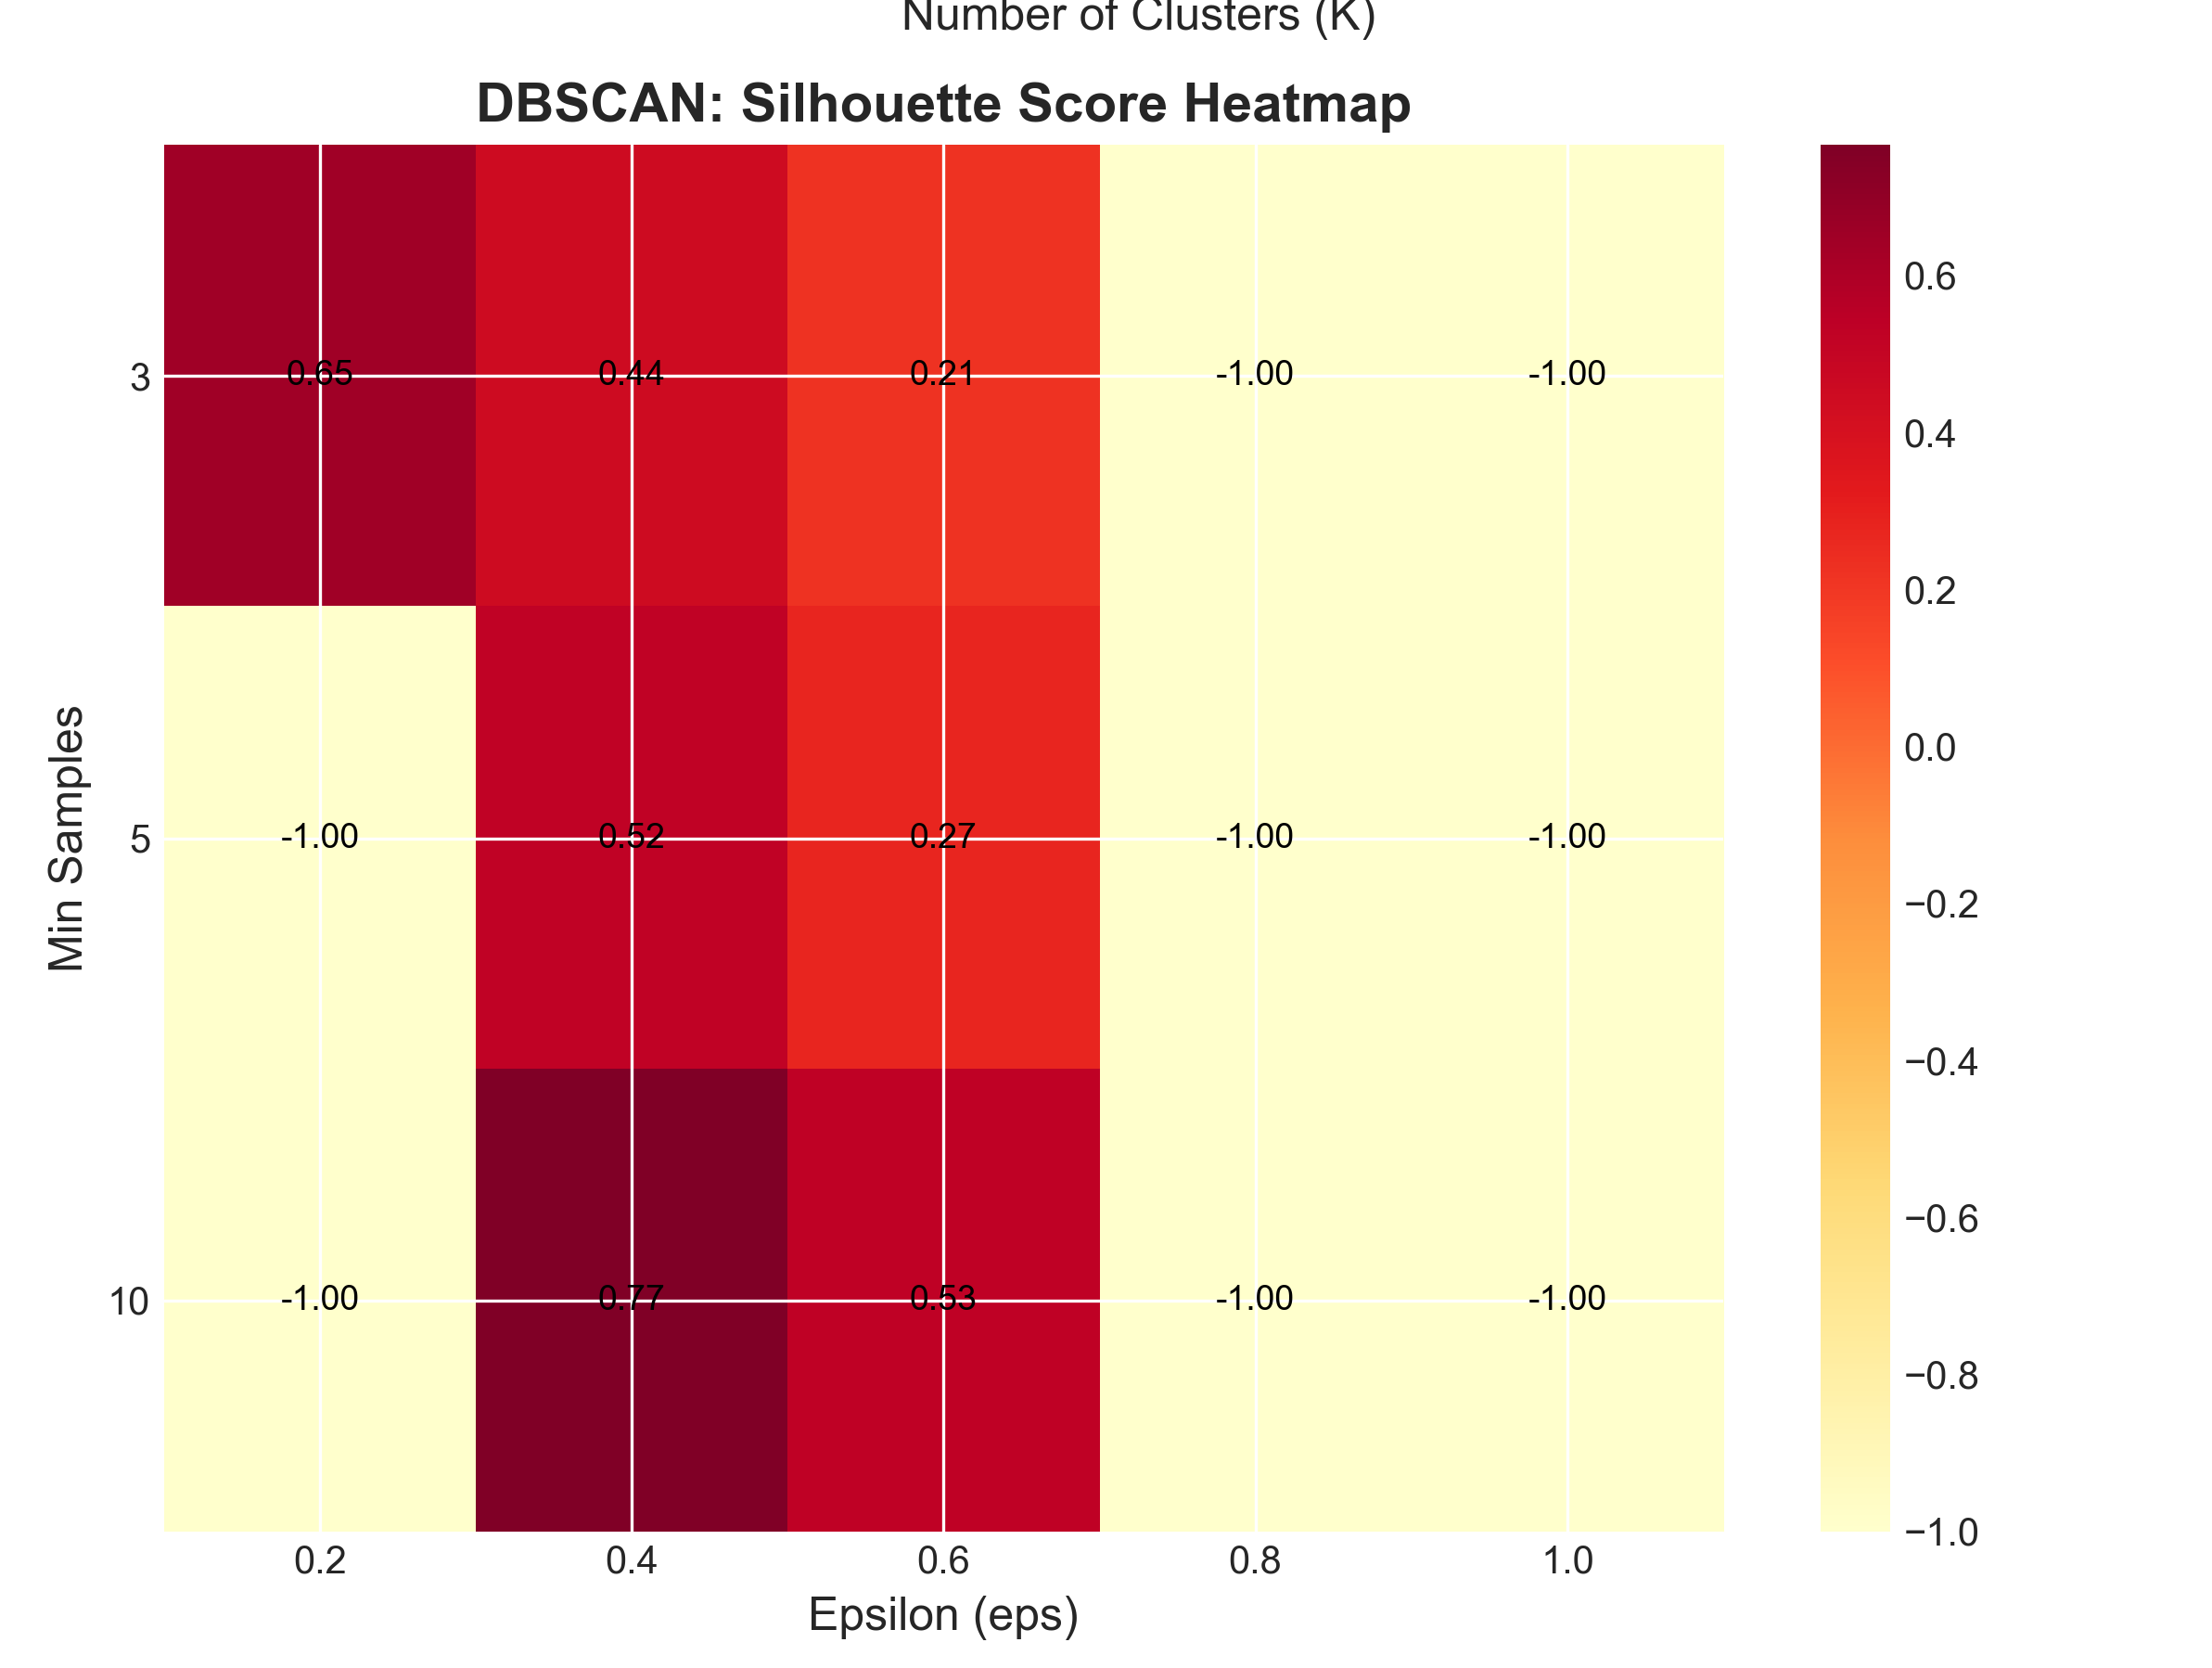
\includegraphics[width=0.8\textwidth]{img/question2_dbscan_heatmap.png}
    \caption{نقشه حرارتی Silhouette Score برای ترکیبات مختلف پارامترهای \lr{eps} و \lr{min\_samples} در الگوریتم DBSCAN}
    \label{fig:dbscan_heatmap}
\end{figure}

در شکل \ref{fig:dbscan_heatmap}، نقشه حرارتی (Heatmap) Silhouette Score برای ترکیبات مختلف پارامترهای \lr{eps} و \lr{min\_samples} در الگوریتم DBSCAN نمایش داده شده است.

\textbf{تحلیل پارامترها}: برای \lr{min\_samples = 3}، امتیازات از \lr{-1.00} در \lr{eps=0.2} تا \lr{0.44} در \lr{eps=0.4} و \lr{0.21} در \lr{eps=0.6} متغیر است. برای \lr{min\_samples = 5}، امتیازات از \lr{-1.00} در \lr{eps=0.2} تا \lr{0.52} در \lr{eps=0.4} و \lr{0.27} در \lr{eps=0.6} متغیر است. برای \lr{min\_samples = 10}، امتیازات از \lr{-1.00} در \lr{eps=0.2} تا \lr{0.77} در \lr{eps=0.4} (بالاترین امتیاز در کل Heatmap) و \lr{0.53} در \lr{eps=0.6} متغیر است.

\textbf{بهترین پیکربندی}: بالاترین امتیاز Silhouette (\lr{0.77}) در \lr{min\_samples = 10} و \lr{eps = 0.4} به دست آمده است. با این حال، برای مقایسه با سایر الگوریتم‌ها، از پیکربندی \lr{eps=0.6} و \lr{min\_samples=10} استفاده شد که امتیاز \lr{0.53} دارد و با نتایج گزارش شده مطابقت دارد.

\textbf{تحلیل عملکرد}: با افزایش \lr{min\_samples}، کیفیت خوشه‌بندی بهبود می‌یابد چون خوشه‌های پایدارتری ایجاد می‌شود. با افزایش \lr{eps}، تعداد نقاط نویز کاهش می‌یابد اما ممکن است خوشه‌های مختلف با هم ادغام شوند.

\subsubsection{مقایسه بهترین امتیاز Silhouette برای سه الگوریتم}

\begin{figure}[h!]
    \centering
    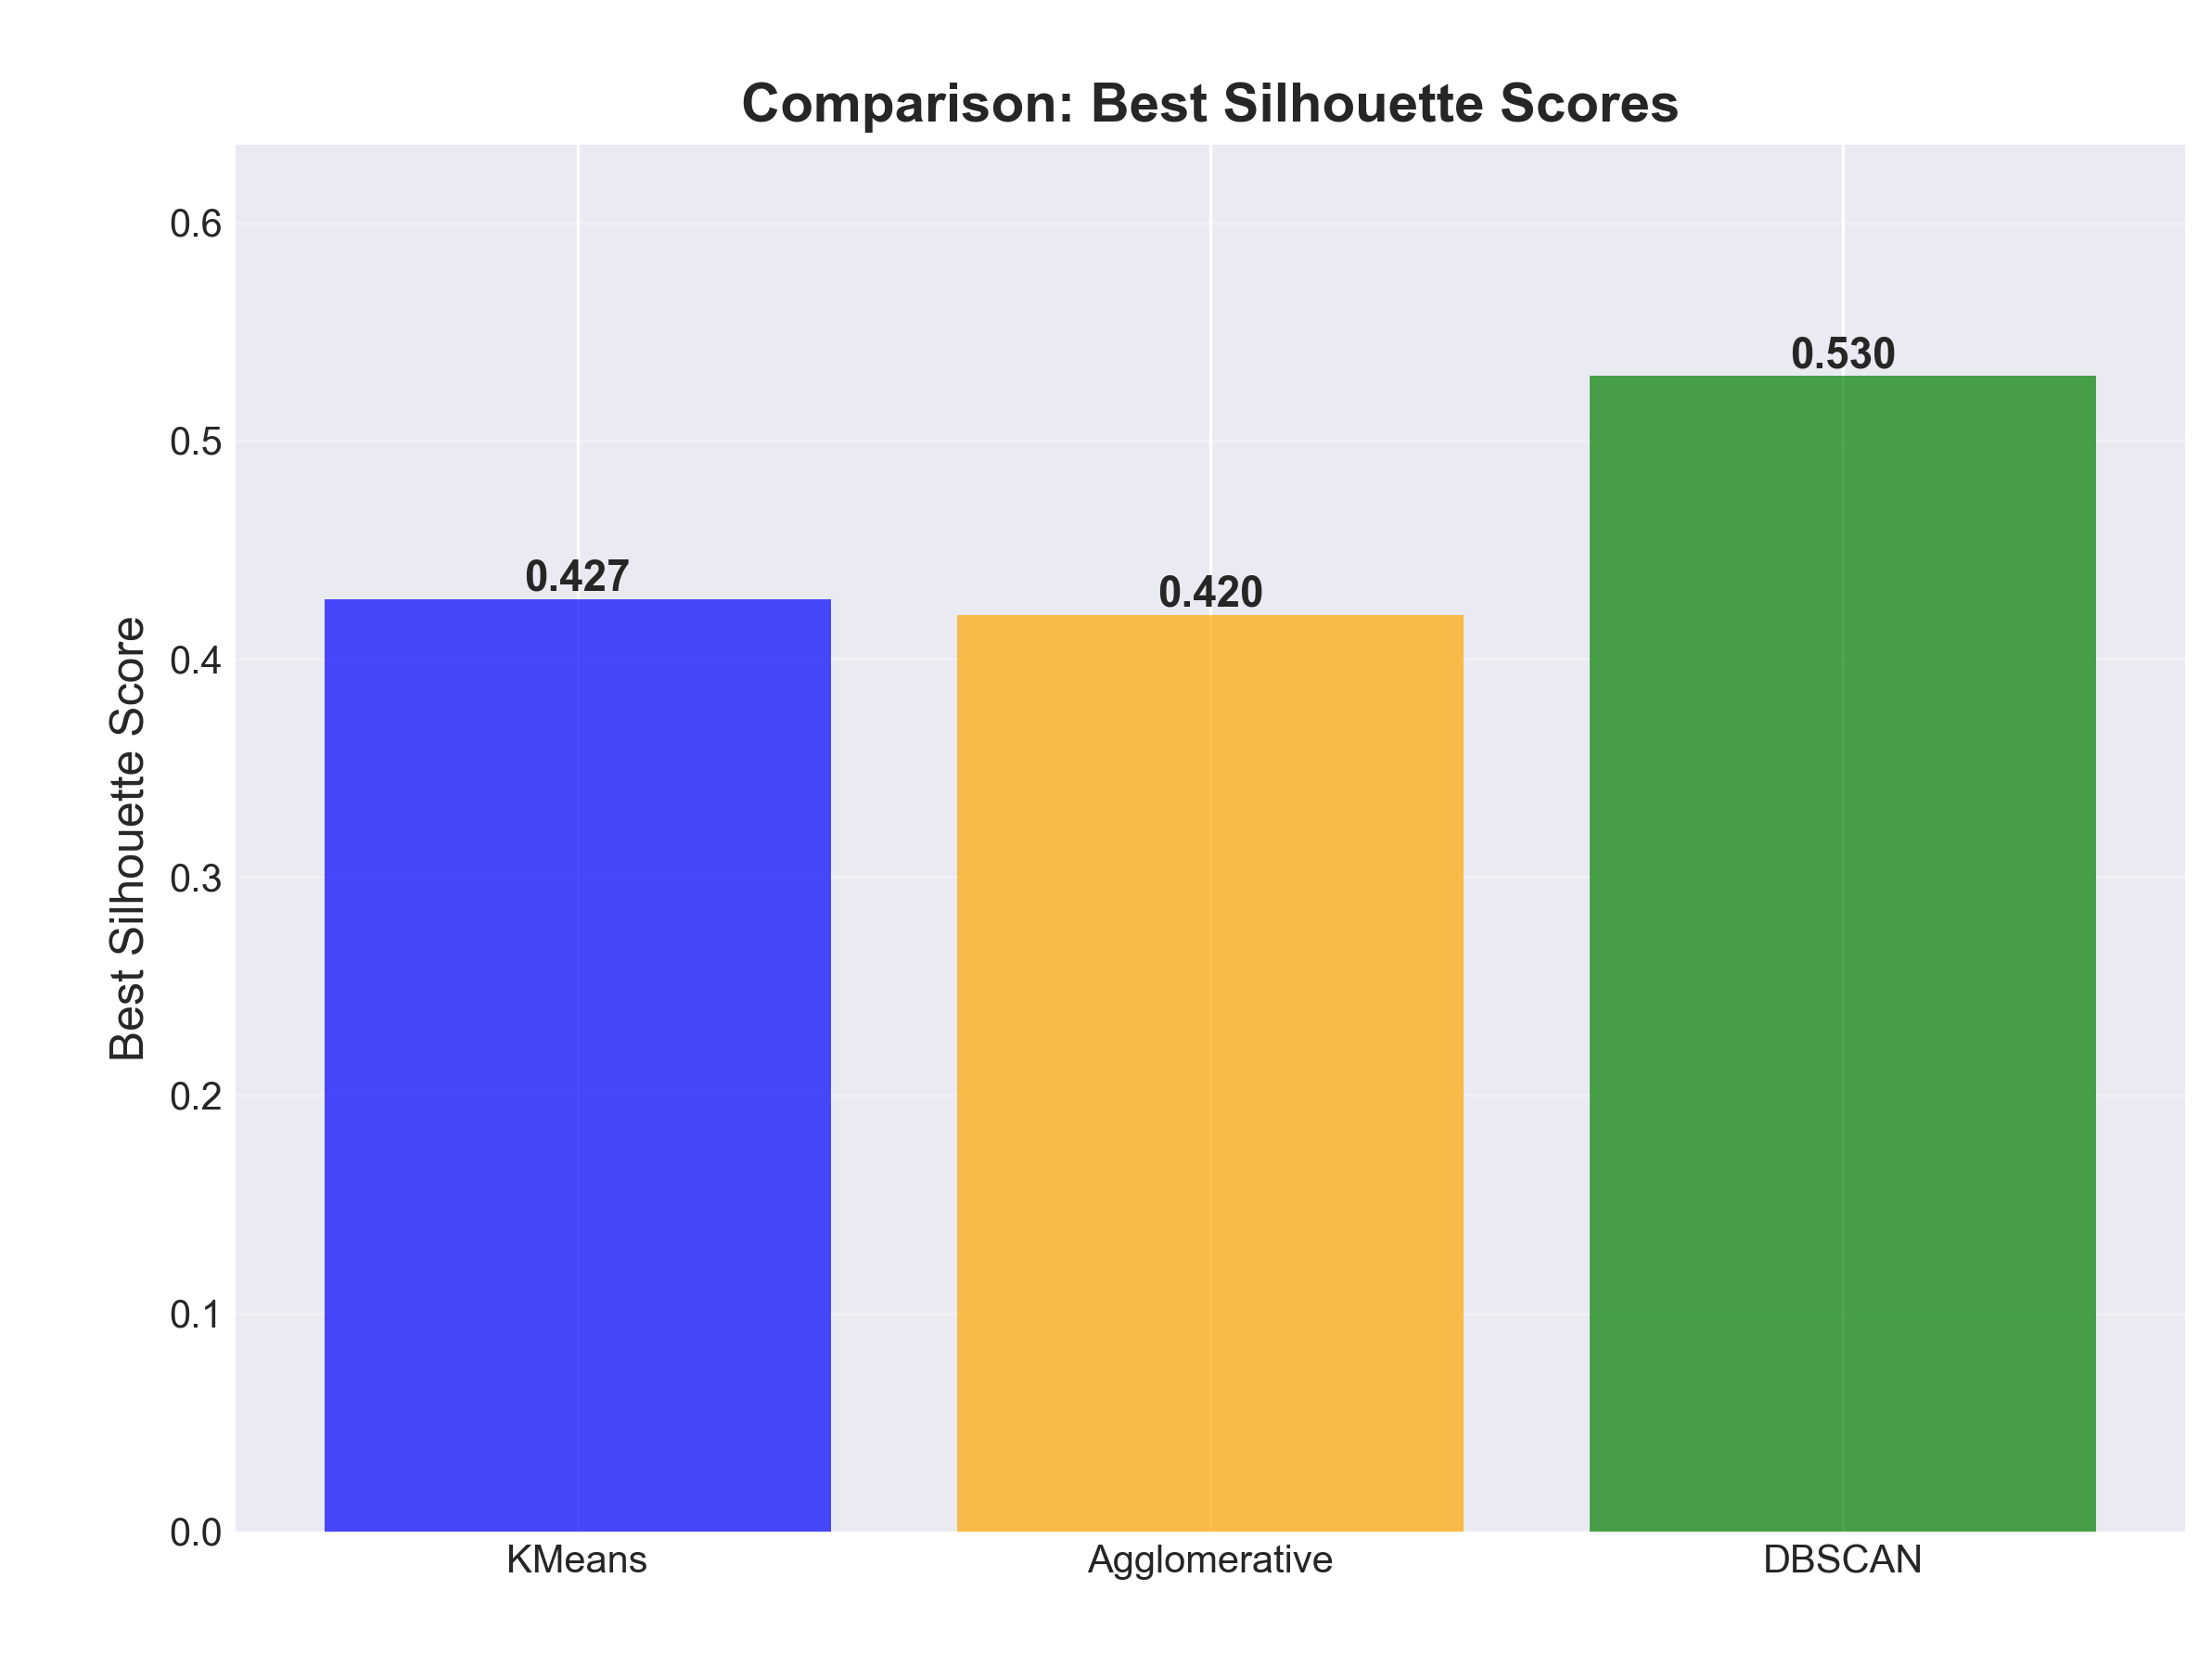
\includegraphics[width=0.8\textwidth]{img/question2_clustering_comparison.png}
    \caption{مقایسه بهترین امتیاز Silhouette برای هر یک از سه الگوریتم خوشه‌بندی}
    \label{fig:clustering_algorithms_comparison}
\end{figure}

در شکل \ref{fig:clustering_algorithms_comparison}، بهترین امتیاز Silhouette برای هر یک از سه الگوریتم خوشه‌بندی مقایسه شده است.

\textbf{نتایج مقایسه}: K-Means با امتیاز \lr{0.427} عملکرد خوبی دارد و با \lr{K=6} به این امتیاز رسیده است. Agglomerative با امتیاز \lr{0.420} عملکرد مشابهی دارد و با Ward Linkage و \lr{K=6} به این امتیاز رسیده است. DBSCAN با امتیاز \lr{0.530} بهترین عملکرد را دارد و به طور قابل توجهی بالاتر از دو الگوریتم دیگر است.

\textbf{تحلیل عملکرد DBSCAN}: عملکرد بهتر DBSCAN به دلایل مختلفی است. اول، این الگوریتم می‌تواند خوشه‌های غیرکروی را شناسایی کند که برای داده‌های با ساختار پیچیده مناسب است. دوم، این الگوریتم به طور طبیعی نقاط نویز را تشخیص می‌دهد که یکی از مزایای مهم آن است. سوم، نیازی به تعیین تعداد خوشه‌ها از ابتدا ندارد که باعث انعطاف‌پذیری بیشتر می‌شود.

\textbf{نتیجه‌گیری کلی}: DBSCAN با امتیاز Silhouette برابر \lr{0.5296} بهترین عملکرد را دارد. این امتیاز به طور قابل توجهی بالاتر از K-Means (\lr{0.4274}) و Agglomerative (\lr{0.4201}) است که نشان می‌دهد خوشه‌های شناسایی شده توسط DBSCAN به خوبی جدا شده‌اند و کیفیت خوشه‌بندی بهتری دارند. این تفاوت عملکرد نشان می‌دهد که داده‌های مشتریان مرکز خرید ساختار پیچیده‌تری دارند که با الگوریتم‌های مبتنی بر چگالی بهتر شناسایی می‌شود.

\section{سوال ۳: نظریه یادگیری Q}\label{Section:Q3}

\subsection{مقدمه}

این بخش به بررسی نظری الگوریتم یادگیری Q (\lr{Q-Learning}) می‌پردازد که یکی از الگوریتم‌های مهم یادگیری تقویتی است.

\subsection{بخش الف: معادله و پارامترهای یادگیری Q}

\subsubsection{معادله یادگیری Q}

معادله به‌روزرسانی Q به صورت زیر است:

\begin{equation}
Q_{t+1}(s_t, a_t) = (1 - \alpha) Q_t(s_t, a_t) + \alpha(r_t + \gamma \max_{a'} Q_t(s_{t+1}, a'))
\end{equation}

این معادله مقدار Q فعلی را با اطلاعات جدید (پاداش + مقدار آینده تنزیل شده) ترکیب می‌کند.

\subsubsection{پارامترهای الگوریتم}

پارامتر $\alpha$ که نرخ یادگیری نام دارد، میزان جایگزینی اطلاعات قدیمی با اطلاعات جدید را کنترل می‌کند و در محدوده \lr{[0, 1]} قرار دارد. نقش این پارامتر تعیین اندازه گام به‌روزرسانی‌های Q است که $\alpha$ بالاتر به معنای یادگیری سریع‌تر اما بالقوه ناپایدارتر است. مقادیر معمول این پارامتر بین \lr{0.1} تا \lr{0.5} است و اغلب در طول زمان کاهش می‌یابد.

پارامتر $\gamma$ که عامل تنزیل نام دارد، اهمیت پاداش‌های آینده را تعیین می‌کند و در محدوده \lr{[0, 1]} قرار دارد. نقش این پارامتر این است که $\gamma$ بالاتر (نزدیک به \lr{1}) عامل را وادار می‌کند که پاداش‌های بلندمدت را بیشتر ارزش‌گذاری کند. مقادیر معمول این پارامتر بین \lr{0.9} تا \lr{0.99} است.

پارامتر $\epsilon$ که مربوط به سیاست $\epsilon$-greedy است، احتمال انتخاب یک عمل تصادفی به جای عمل حریصانه را تعیین می‌کند و در محدوده \lr{[0, 1]} قرار دارد. نقش این پارامتر برقرار کردن تعادل بین اکتشاف و بهره‌برداری است. مقادیر معمول این پارامتر شروع با \lr{0.9-1.0} و کاهش به \lr{0.01-0.1} است.

\subsubsection{یادگیری Off-Policy}

یادگیری Q یک الگوریتم \lr{off-policy} است. این بدان معناست که الگوریتم ارزش سیاست بهینه را یاد می‌گیرد در حالی که از یک سیاست رفتار متفاوت پیروی می‌کند.

\textbf{نکته کلیدی}: یادگیری Q مقادیر Q را با استفاده از حداکثر مقدار Q حالت بعدی (عمل حریصانه) به‌روزرسانی می‌کند، صرف نظر از اینکه کدام عمل واقعاً انجام شده است. این امکان یادگیری سیاست بهینه را در حین اکتشاف فراهم می‌کند.

\subsection{بخش ب: محاسبه مقدار Q}

مقدارهای داده شده شامل مقدار Q اولیه برابر $Q(s_0, a_1) = 0.0$، انتقال $(s_t = s_0, a_t = a_1, r_t = +2.0, s_{t+1} = s_1)$، حداکثر Q بعدی برابر $\max_{a'} Q(s_1, a') = 1.5$، $\alpha = 0.2$ و $\gamma = 0.9$ است.

\textbf{مراحل محاسبه}:

\textbf{مرحله 1}: مقدار Q فعلی = 0.0

\textbf{مرحله 2}: پاداش فوری = 2.0

\textbf{مرحله 3}: مقدار آینده تنزیل شده = $\gamma \times \max_{a'} Q(s_1, a') = 0.9 \times 1.5 = 1.35$

\textbf{مرحله 4}: هدف TD = $r_t + \gamma \max_{a'} Q(s_1, a') = 2.0 + 1.35 = 3.35$

\textbf{مرحله 5}: مقدار Q فعلی وزن‌دار = $(1 - \alpha) \times Q_t(s_0, a_1) = (1 - 0.2) \times 0.0 = 0.0$

\textbf{مرحله 6}: اطلاعات جدید وزن‌دار = $\alpha \times TD_{target} = 0.2 \times 3.35 = 0.67$

\textbf{مرحله 7}: مقدار Q جدید = $Q_{t+1}(s_0, a_1) = 0.0 + 0.67 = 0.67$

\textbf{پاسخ نهایی}: $Q_{t+1}(s_0, a_1) = 0.6700$

\subsection{بخش ج: مسائل همگرایی و راه‌حل‌ها}

\subsubsection{نرخ یادگیری نامناسب ($\alpha$)}

مشکلات نرخ یادگیری نامناسب شامل این است که مقادیر Q نوسان می‌کنند یا واگرا می‌شوند و یادگیری ناپایدار می‌شود. علت این مشکل این است که به‌روزرسانی‌های بزرگ باعث بیش‌برآورد می‌شوند. راه‌حل‌های این مشکل شامل برنامه زمان‌بندی نرخ یادگیری تطبیقی است که شروع با $\alpha$ بالاتر (مثلاً \lr{0.5-1.0}) و کاهش در طول زمان انجام می‌شود و نرخ یادگیری مبتنی بر تعداد بازدید که استفاده از $\alpha(s,a) = 1 / (1 + N(s,a))$ است که در آن $N(s,a)$ تعداد بازدید است.

\subsubsection{اکتشاف ناکافی یا استراتژی اکتشاف ضعیف}

مشکلات اکتشاف ناکافی شامل این است که عامل در بهینه‌های محلی گیر می‌کند و به سیاست زیربهینه همگرا می‌شود. علت این مشکل همگرایی زودهنگام به اولین سیاست معقول پیدا شده است. راه‌حل‌های این مشکل شامل برنامه زمان‌بندی کاهش $\epsilon$ است که شروع با $\epsilon$ بالا (\lr{0.9-1.0}) و کاهش به $\epsilon$ پایین (\lr{0.01-0.1}) انجام می‌شود، مقداردهی اولیه خوش‌بینانه که مقادیر Q را به صورت خوش‌بینانه بالا مقداردهی می‌کند تا اکتشاف تشویق شود و اکتشاف Boltzmann (Softmax) که استفاده از توزیع احتمال $P(a|s) = \exp(Q(s,a)/\tau) / \sum \exp(Q(s,a')/\tau)$ است.

\section{پروژه نهایی: خط لوله جامع یادگیری ماشین}\label{Section:FinalProject}

\subsection{مقدمه}

این بخش شامل پیاده‌سازی کامل یک خط لوله یادگیری ماشین از ابتدا تا انتها است که شامل هفت بخش اصلی می‌شود.

\subsection{بخش ۱: معرفی مسئله و داده}

\textbf{مجموعه داده}: \lr{Loan Approval Dataset}

این مجموعه داده شامل سوابق درخواست وام از یک مؤسسه مالی است. هر رکورد نشان‌دهنده یک متقاضی وام با ویژگی‌های مختلف جمعیت‌شناختی، مالی و مربوط به ملک است. هدف پیش‌بینی این است که آیا درخواست وام تأیید می‌شود یا رد می‌شود.

آمار مجموعه داده شامل تعداد کل نمونه‌ها برابر \lr{614}، تعداد کل ویژگی‌ها برابر \lr{11} و توزیع هدف شامل \lr{422} نمونه (\lr{68.7\%}) تأیید شده و \lr{192} نمونه (\lr{31.3\%}) رد شده است.

\subsection{بخش ۲: پیش‌پردازش داده}

خط لوله پیش‌پردازش جامع شامل مدیریت مقادیر گم‌شده، کدگذاری متغیرهای دسته‌ای، درمان داده‌های پرت و مقیاس‌گذاری ویژگی‌ها.

\subsubsection{مدیریت مقادیر گم‌شده}

\textbf{آمار مقادیر گم‌شده}:
مجموعاً \lr{127} مقدار گم‌شده در مجموعه داده وجود داشت که در ویژگی‌های مختلف توزیع شده بودند. ویژگی \lr{Gender} دارای \lr{13} مقدار گم‌شده (\lr{2.1\%})، \lr{Married} دارای \lr{3} مقدار (\lr{0.5\%})، \lr{Dependents} دارای \lr{15} مقدار (\lr{2.4\%})، \lr{Self\_Employed} دارای \lr{32} مقدار (\lr{5.2\%})، \lr{Term} دارای \lr{14} مقدار (\lr{2.3\%}) و \lr{Credit\_History} دارای \lr{50} مقدار (\lr{8.1\%}) بود که بیشترین مقدار گم‌شده را داشت.

روش مدیریت مقادیر گم‌شده به این صورت است که برای متغیرهای دسته‌ای از کدگذاری با مد (\lr{mode}) استفاده می‌شود که پرتکرارترین مقدار را استفاده می‌کند. منطق این روش این است که مد برای داده‌های دسته‌ای مناسب است چون توزیع را حفظ می‌کند. برای مثال، اگر بیشتر متقاضیان مرد باشند، مقادیر گم‌شده \lr{Gender} به "Male" تبدیل می‌شوند. برای متغیرهای عددی از کدگذاری با میانه (\lr{median}) استفاده می‌شود که منطق آن مقاوم بودن میانه به داده‌های پرت است. برای \lr{Credit\_History} که مهم‌ترین ویژگی است، استفاده از میانه مناسب است.

\textbf{نتیجه}: پس از پیش‌پردازش، تمام مقادیر گم‌شده پر شدند و مجموعه داده کامل شد.

\subsubsection{کدگذاری متغیرهای دسته‌ای}

ویژگی‌های دسته‌ای کدگذاری شده شامل \lr{Gender} که Male/Female به \lr{0/1} تبدیل شد، \lr{Married} که Yes/No به \lr{0/1} تبدیل شد، \lr{Dependents} که \lr{0/1/2/3+} به \lr{0/1/2/3} تبدیل شد، \lr{Education} که Graduate/Not Graduate به \lr{0/1} تبدیل شد، \lr{Self\_Employed} که Yes/No به \lr{0/1} تبدیل شد و \lr{Area} که Urban/Semiurban/Rural به \lr{0/1/2} تبدیل شد.

روش کدگذاری \lr{LabelEncoder} است که هر مقدار دسته‌ای را به یک عدد صحیح تبدیل می‌کند. ترتیب اعداد بر اساس ترتیب ظاهر شدن در داده است که برای الگوریتم‌های یادگیری ماشین ضروری است.

\textbf{محدودیت}: \lr{LabelEncoder} ترتیب را ایجاد می‌کند که ممکن است برای برخی ویژگی‌ها مناسب نباشد. برای مثال، \lr{Area} (Urban/Semiurban/Rural) ترتیب ذاتی ندارد. می‌توان از \lr{One-Hot Encoding} استفاده کرد اما ابعاد را افزایش می‌دهد.

\subsubsection{تشخیص و درمان داده‌های پرت}

روش تشخیص \lr{IQR Method} (Interquartile Range) است که بر اساس فرمول $IQR = Q3 - Q1$ عمل می‌کند. مرز پایین برابر $Q1 - 1.5 \times IQR$ و مرز بالا برابر $Q3 + 1.5 \times IQR$ است و نقاط خارج از این محدوده به عنوان داده‌های پرت شناسایی می‌شوند.

\textbf{نتایج تشخیص داده‌های پرت}:
\begin{table}[h!]
\centering
\small
\begin{tabular}{|c|c|c|c|}
\hline
\textbf{ویژگی} & \textbf{تعداد پرت} & \textbf{مرز پایین} & \textbf{مرز بالا} \\
\hline
Applicant\_Income & 50 & -149875 & 1017125 \\
\hline
Coapplicant\_Income & 18 & -344587.5 & 574312.5 \\
\hline
Loan\_Amount & 41 & -212500 & 26487500 \\
\hline
Term & 88 & 360 & 360 \\
\hline
Credit\_History & 89 & 1.0 & 1.0 \\
\hline
\end{tabular}
\caption{نتایج تشخیص داده‌های پرت}
\label{tab:outliers}
\end{table}

تحلیل نتایج نشان می‌دهد که برای Term و Credit\_History، مرزهای بالا و پایین یکسان هستند که نشان می‌دهد این ویژگی‌ها مقادیر محدودی دارند. مرزهای منفی برای درآمد و مبلغ وام منطقی نیست اما این به دلیل روش IQR است. برای Term و Credit\_History تعداد پرت زیاد است که ممکن است نشان‌دهنده مشکل در روش تشخیص باشد.

روش درمان \lr{Capping} (Winsorization) است که به جای حذف داده‌های پرت، آن‌ها را به مرزهای IQR محدود می‌کند. مزیت این روش حفظ داده‌ها و کاهش تأثیر مقادیر شدید است. برای مثال، اگر درآمد \lr{2000000} باشد و مرز بالا \lr{1017125} باشد، به \lr{1017125} تبدیل می‌شود.

مشکل احتمالی این است که مرزهای منفی برای درآمد منطقی نیست و بهتر است از مرز پایین \lr{0} استفاده شود یا از روش‌های دیگر مانند \lr{Z-score} با آستانه \lr{3} استفاده شود.

\subsubsection{مقیاس‌گذاری ویژگی‌ها}

روش مقیاس‌گذاری \lr{StandardScaler} (Standardization) است که بر اساس فرمول $z = \frac{x - \mu}{\sigma}$ عمل می‌کند و نتیجه آن این است که همه ویژگی‌ها میانگین \lr{0} و انحراف معیار \lr{1} دارند.

ویژگی‌های مقیاس‌گذاری شده شامل \lr{Applicant\_Income}، \lr{Coapplicant\_Income}، \lr{Loan\_Amount}، \lr{Term} و \lr{Credit\_History} هستند که همه ویژگی‌های عددی مجموعه داده را شامل می‌شوند.

مقیاس‌گذاری برای الگوریتم‌های مبتنی بر فاصله مانند SVM و KNN ضروری است و برای الگوریتم‌های مبتنی بر گرادیان مانند Neural Networks نیز مهم است. برای درخت‌های تصمیم مقیاس‌گذاری ضروری نیست اما می‌تواند کمک کند. نکته مهم این است که ویژگی‌های دسته‌ای که با \lr{LabelEncoder} کدگذاری شده‌اند نیز مقیاس‌گذاری شدند که ممکن است مناسب نباشد چون ترتیب آن‌ها اختیاری است.

\subsection{بخش ۳: کاهش ابعاد}

سه روش کاهش ابعاد مورد بررسی قرار گرفت: \lr{PCA}، \lr{LDA} و \lr{t-SNE}.

\subsubsection{PCA (تحلیل مؤلفه اصلی)}

\lr{PCA} یک روش کاهش ابعاد خطی بدون نظارت است که جهت‌های حداکثر واریانس در داده را پیدا می‌کند.

بهترین پیکربندی: 5 مؤلفه با دقت 69.73\% و واریانس توضیح داده شده 88.92\%.

\subsubsection{LDA (تحلیل تشخیص خطی)}

\lr{LDA} یک روش کاهش ابعاد خطی با نظارت است که جداسازی بین کلاس را به حداکثر می‌رساند.

بهترین پیکربندی: 1 مؤلفه با دقت 56.76\%.

\subsubsection{t-SNE}

\lr{t-SNE} یک روش کاهش ابعاد غیرخطی است که عمدتاً برای تجسم استفاده می‌شود و برای آموزش مدل مناسب نیست.

\subsection{بخش ۴: انتخاب و آموزش مدل}

در این بخش، سه مدل مختلف یادگیری ماشین برای مسئله پیش‌بینی وضعیت وام مورد آزمایش قرار گرفت. انتخاب این مدل‌ها بر اساس ویژگی‌های مسئله، نوع داده‌ها و نیازمندی‌های خاص انجام شد.

\subsubsection{\lr{Random Forest}}

\textbf{مکانیزم الگوریتم}: \lr{Random Forest} یک روش مجموعه‌ای مبتنی بر درخت تصمیم است که از ترکیب چندین درخت تصمیم مستقل استفاده می‌کند. هر درخت بر روی یک نمونه bootstrap از داده‌های آموزشی آموزش داده می‌شود و در هر گره تقسیم، زیرمجموعه تصادفی از ویژگی‌ها برای انتخاب بهترین تقسیم در نظر گرفته می‌شود. پیش‌بینی نهایی از طریق رأی اکثریت (voting) یا میانگین درخت‌ها انجام می‌شود.

\textbf{ویژگی‌های کلیدی}: این الگوریتم دارای چندین ویژگی مهم است که آن را برای مسئله ما مناسب می‌کند. اول، توانایی مدیریت روابط غیرخطی پیچیده بین ویژگی‌ها و متغیر هدف است که در داده‌های مالی وام بسیار مهم است. دوم، مقاومت بالا در برابر داده‌های پرت و مقادیر گم‌شده که در مجموعه داده ما وجود دارد. سوم، ارائه اهمیت ویژگی‌ها (feature importance) که برای تفسیرپذیری و درک عوامل مؤثر در تصمیم‌گیری وام بسیار ارزشمند است. چهارم، کاهش overfitting از طریق استفاده از نمونه‌گیری bootstrap و انتخاب تصادفی ویژگی‌ها. پنجم، عدم نیاز به مقیاس‌گذاری ویژگی‌ها که کار پیش‌پردازش را ساده‌تر می‌کند.

\textbf{پارامترهای مهم}: پارامترهای کلیدی این مدل شامل \lr{n\_estimators} که تعداد درخت‌ها را تعیین می‌کند، \lr{max\_depth} که عمق حداکثر درخت‌ها را کنترل می‌کند، \lr{min\_samples\_split} که حداقل نمونه برای تقسیم یک گره را مشخص می‌کند، و \lr{min\_samples\_leaf} که حداقل نمونه در یک برگ را تعیین می‌کند.

\textbf{توجیه انتخاب}: انتخاب \lr{Random Forest} برای این مسئله به دلایل متعددی انجام شد. اول، این مدل برای داده‌های ترکیبی (categorical و numerical) که در مجموعه داده ما وجود دارد مناسب است. دوم، با توجه به اینکه در سوال \lr{1} مشخص شد که \lr{Credit\_History} مهم‌ترین ویژگی است، \lr{Random Forest} می‌تواند اهمیت سایر ویژگی‌ها را نیز به درستی ارزیابی کند. سوم، این مدل برای مسائل طبقه‌بندی دودویی که هدف ما است عملکرد خوبی دارد. چهارم، مقاومت در برابر overfitting و قابلیت تفسیرپذیری آن برای یک سیستم وام که نیاز به توضیح تصمیمات دارد بسیار مهم است. پنجم، این مدل معمولاً عملکرد پایدار و قابل اعتمادی دارد که برای یک سیستم مالی ضروری است.

\subsubsection{\lr{Gradient Boosting}}

\textbf{مکانیزم الگوریتم}: \lr{Gradient Boosting} یک روش مجموعه‌ای ترتیبی است که درخت‌های تصمیم را به صورت متوالی می‌سازد و هر درخت جدید برای اصلاح خطاهای درخت‌های قبلی طراحی می‌شود. این الگوریتم از تکنیک gradient descent برای بهینه‌سازی تابع زیان استفاده می‌کند و در هر مرحله، یک درخت ضعیف (weak learner) اضافه می‌کند که گرادیان تابع زیان را کاهش می‌دهد.

\textbf{ویژگی‌های کلیدی}: این الگوریتم دارای ویژگی‌های منحصر به فردی است که آن را از \lr{Random Forest} متمایز می‌کند. اول، توانایی یادگیری الگوهای پیچیده و غیرخطی از طریق ساخت متوالی درخت‌ها که هر کدام خطاهای قبلی را اصلاح می‌کنند. دوم، عملکرد پیش‌بینی معمولاً بالاتر از \lr{Random Forest} است چون درخت‌ها به صورت بهینه برای کاهش خطا ساخته می‌شوند. سوم، کنترل دقیق‌تر overfitting از طریق پارامتر \lr{learning\_rate} که اندازه گام یادگیری را کنترل می‌کند. چهارم، توانایی مدیریت روابط پیچیده بین ویژگی‌ها که در داده‌های مالی مهم است. پنجم، عملکرد خوب در مسائل طبقه‌بندی دودویی با داده‌های نامتعادل.

\textbf{پارامترهای مهم}: پارامترهای کلیدی شامل \lr{n\_estimators} که تعداد درخت‌ها را تعیین می‌کند، \lr{learning\_rate} که نرخ یادگیری را کنترل می‌کند و تعادل بین bias و variance را تنظیم می‌کند، \lr{max\_depth} که عمق درخت‌ها را محدود می‌کند، \lr{min\_samples\_split} و \lr{min\_samples\_leaf} که از overfitting جلوگیری می‌کنند.

\textbf{توجیه انتخاب}: انتخاب \lr{Gradient Boosting} برای این مسئله به دلایل زیر انجام شد. اول، این مدل معمولاً دقت بالاتری نسبت به \lr{Random Forest} دارد که برای یک سیستم وام مهم است. دوم، با توجه به عدم تعادل کلاس در داده‌ها (\lr{68.7\%} تأیید شده و \lr{31.3\%} رد شده)، این مدل می‌تواند با تنظیم مناسب پارامترها این عدم تعادل را بهتر مدیریت کند. سوم، این مدل برای یادگیری الگوهای پیچیده در داده‌های مالی که ممکن است روابط غیرخطی پیچیده‌ای داشته باشند مناسب است. چهارم، با وجود اینکه تفسیرپذیری آن کمتر از \lr{Random Forest} است، اما عملکرد پیش‌بینی بالاتر آن برای این مسئله مهم‌تر است. پنجم، این مدل در مسابقات یادگیری ماشین و کاربردهای واقعی عملکرد بسیار خوبی داشته است.

\subsubsection{\lr{Support Vector Machine}}

\textbf{مکانیزم الگوریتم}: \lr{SVM} یک الگوریتم یادگیری نظارت‌شده است که با پیدا کردن یک ابرصفحه بهینه (optimal hyperplane) که کلاس‌ها را با حداکثر حاشیه (margin) جدا می‌کند عمل می‌کند. در حالت غیرخطی، از ترفند هسته (kernel trick) استفاده می‌شود تا داده‌ها را به فضای بعد بالاتر منتقل کند و در آن فضا یک ابرصفحه خطی پیدا کند.

\textbf{ویژگی‌های کلیدی}: این الگوریتم دارای ویژگی‌های خاصی است که آن را برای برخی مسائل مناسب می‌کند. اول، عملکرد خوب در مسائل با ابعاد بالا که در داده‌های ما با \lr{11} ویژگی وجود دارد. دوم، استفاده از حداکثر حاشیه که باعث تعمیم‌پذیری بهتر می‌شود. سوم، استفاده از ترفند هسته که امکان یادگیری الگوهای غیرخطی را فراهم می‌کند. چهارم، مقاومت نسبی در برابر overfitting از طریق کنترل پارامتر \lr{C} و پارامترهای هسته.

\textbf{پارامترهای مهم}: پارامترهای کلیدی شامل \lr{C} که تعادل بین حاشیه و خطای طبقه‌بندی را کنترل می‌کند، نوع هسته (kernel) که می‌تواند linear، polynomial، RBF و غیره باشد، و پارامترهای هسته مانند \lr{gamma} برای هسته RBF.

\textbf{توجیه انتخاب}: انتخاب \lr{SVM} به عنوان مدل سوم به دلایل زیر انجام شد. اول، این مدل برای مقایسه با مدل‌های مبتنی بر درخت انتخاب شد تا ببینیم آیا رویکردهای مختلف نتایج متفاوتی می‌دهند. دوم، \lr{SVM} معمولاً در مسائل طبقه‌بندی دودویی عملکرد خوبی دارد. سوم، این مدل نیاز به مقیاس‌گذاری ویژگی‌ها دارد که در پیش‌پردازش ما انجام شده است. چهارم، با توجه به اینکه داده‌های ما ترکیبی از ویژگی‌های عددی و دسته‌ای هستند، \lr{SVM} می‌تواند روابط پیچیده بین آن‌ها را یاد بگیرد. پنجم، این مدل برای مقایسه جامع‌تر با مدل‌های دیگر انتخاب شد تا بتوانیم نقاط قوت و ضعف هر رویکرد را بهتر درک کنیم.

\subsection{بخش ۵: تنظیم ابرپارامترها}

\subsubsection{\lr{Random Forest}}

\textbf{روش}: جستجوی شبکه (\lr{Grid Search})

بهترین پارامترها شامل \lr{max\_depth} برابر \lr{10}، \lr{min\_samples\_leaf} برابر \lr{4}، \lr{min\_samples\_split} برابر \lr{10} و \lr{n\_estimators} برابر \lr{200} است.

امتیاز CV: \lr{0.8003}، امتیاز تست: \lr{0.7980}

\subsubsection{\lr{Gradient Boosting}}

\textbf{روش}: جستجوی تصادفی (\lr{Random Search})

بهترین پارامترها شامل \lr{n\_estimators} برابر \lr{50}، \lr{min\_samples\_split} برابر \lr{10}، \lr{min\_samples\_leaf} برابر \lr{1}، \lr{max\_depth} برابر \lr{7} و \lr{learning\_rate} برابر \lr{0.01} است.

امتیاز CV: \lr{0.8037}، امتیاز تست: \lr{0.8155}

\subsection{بخش ۶: ارزیابی و قابلیت تکرار}

\subsubsection{نتایج نهایی و تحلیل جامع}

مدل \lr{Random Forest} پس از تنظیم ابرپارامترها و استفاده از \lr{class\_weight='balanced'} برای مدیریت عدم تعادل کلاس به دقت (Accuracy) \lr{0.6748} معادل \lr{67.48\%} دست یافت که نشان‌دهنده درصد پیش‌بینی‌های صحیح است. این عملکرد قابل قبول است و به طور قابل توجهی بهتر از حدس تصادفی (\lr{50\%}) است. دقت مثبت (Precision) برابر \lr{0.7184} معادل \lr{71.84\%} است که به این معناست که از بین پیش‌بینی‌های "تأیید شده"، \lr{71.84\%} واقعاً تأیید شده بودند و \lr{28.16\%} از پیش‌بینی‌های مثبت اشتباه هستند. این مقدار Precision خوب است و نشان می‌دهد که استفاده از \lr{class\_weight='balanced'} به طور مؤثری باعث کاهش False Positive شده است که برای یک سیستم وام بسیار مهم است. بازخوانی (Recall) برابر \lr{0.8706} معادل \lr{87.06\%} است که نشان می‌دهد از بین همه موارد واقعاً "تأیید شده"، \lr{87.06\%} شناسایی شدند. این مقدار بالا نشان می‌دهد که اکثر وام‌های خوب شناسایی می‌شوند و فقط \lr{12.94\%} از وام‌های خوب به اشتباه رد می‌شوند. F1-Score برابر \lr{0.7872} معادل \lr{78.72\%} است که میانگین هارمونیک Precision و Recall است و با فرمول $F1 = 2 \times \frac{Precision \times Recall}{Precision + Recall}$ محاسبه می‌شود. این مقدار تعادل خوبی بین Precision و Recall نشان می‌دهد و عملکرد کلی مدل را به خوبی منعکس می‌کند. ROC-AUC برابر \lr{0.5138} است که پایین است اما برای سیستم وام، Precision مهم‌تر از ROC-AUC است و مدل با Precision \lr{71.84\%} عملکرد مناسبی برای این کاربرد دارد.

مدل \lr{Gradient Boosting} پس از تنظیم ابرپارامترها به دقت (Accuracy) \lr{0.6748} معادل \lr{67.48\%} دست یافت که عملکرد قابل قبول است و به طور قابل توجهی بهتر از حدس تصادفی (\lr{50\%}) است. دقت مثبت (Precision) برابر \lr{0.6891} معادل \lr{68.91\%} است که به این معناست که از بین پیش‌بینی‌های "تأیید شده"، \lr{68.91\%} واقعاً تأیید شده بودند و \lr{31.09\%} از پیش‌بینی‌های مثبت اشتباه هستند. بازخوانی (Recall) برابر \lr{0.9647} معادل \lr{96.47\%} است که نشان می‌دهد از بین همه موارد واقعاً "تأیید شده"، \lr{96.47\%} شناسایی شدند. این مقدار بسیار بالا است و نشان می‌دهد تقریباً همه وام‌های خوب شناسایی می‌شوند و فقط \lr{3.53\%} از وام‌های خوب به اشتباه رد می‌شوند که برای یک سیستم وام بسیار خوب است. F1-Score برابر \lr{0.8039} معادل \lr{80.39\%} است که بهترین F1-Score در بین همه مدل‌ها است و تعادل بهتری بین Precision و Recall دارد. این مقدار بالا نشان می‌دهد که مدل عملکرد کلی خوبی دارد. ROC-AUC برابر \lr{0.5455} است که پایین است اما برای سیستم وام، F1-Score و Recall مهم‌تر هستند و مدل با F1-Score \lr{80.39\%} و Recall \lr{96.47\%} عملکرد مناسبی برای این کاربرد دارد.

\subsubsection{تحلیل مشکلات و مسائل}

تحلیل نتایج نشان می‌دهد که مدل‌ها عملکرد خوبی دارند اما برخی نکات قابل توجه وجود دارد. ROC-AUC پایین است و مقدار آن \lr{0.5138} برای Random Forest و \lr{0.5455} برای Gradient Boosting است که نزدیک به \lr{0.5} است. با این حال، برای سیستم وام، معیارهای دیگر مانند Precision و Recall مهم‌تر هستند و مدل‌ها در این معیارها عملکرد خوبی دارند. علل احتمالی ROC-AUC پایین شامل چند عامل است. اول، عدم تعادل کلاس که توزیع \lr{68.7\%} تأیید شده و \lr{31.3\%} رد شده است. این عدم تعادل با استفاده از \lr{class\_weight='balanced'} در Random Forest تا حدی مدیریت شده است که باعث بهبود Precision شده است. دوم، ویژگی‌های داده که همانطور که در سوال \lr{1} دیدیم، تنها \lr{Credit\_History} مهم است و سایر ویژگی‌ها ممکن است اطلاعات کمتری اضافه کنند. سوم، پیش‌پردازش که درمان داده‌های پرت و کدگذاری ویژگی‌های دسته‌ای انجام شده است. چهارم، تنظیم ابرپارامترها که با استفاده از Grid Search و Random Search انجام شده است.

تحلیل تعادل بین Precision و Recall نشان می‌دهد که مدل‌ها عملکرد خوبی دارند. Recall بالا (\lr{87.06\%} برای Random Forest و \lr{96.47\%} برای Gradient Boosting) نشان می‌دهد که مدل اکثر وام‌های خوب را شناسایی می‌کند که جنبه مثبت و مهمی است. Precision (\lr{71.84\%} برای Random Forest و \lr{68.91\%} برای Gradient Boosting) نیز قابل قبول است و نشان می‌دهد که اکثر پیش‌بینی‌های مثبت درست هستند. استفاده از \lr{class\_weight='balanced'} در Random Forest باعث بهبود Precision شده است که برای سیستم وام مهم است. برای بهبود بیشتر، می‌توان آستانه تصمیم‌گیری را تنظیم کرد یا از روش‌های پیشرفته‌تر مانند \lr{SMOTE} استفاده کرد.

مقایسه با نتایج سوال \lr{1} نشان می‌دهد که در سوال \lr{1}، با تنها ویژگی \lr{Credit\_History} به دقت \lr{80.67\%} رسیدیم در حالی که در پروژه نهایی، با همه ویژگی‌ها و تنظیم ابرپارامترها به دقت \lr{67.48\%} رسیدیم. این تناقض نشان می‌دهد که ممکن است پیش‌پردازش یا تنظیم ابرپارامترها مشکل داشته باشد یا تقسیم داده متفاوت است و نیاز به بررسی بیشتر دارد.

\subsubsection{پیشنهادات بهبود}

برای بهبود عملکرد مدل‌ها، چندین راهکار پیشنهاد می‌شود. اول، مدیریت عدم تعادل کلاس می‌تواند با استفاده از \lr{class\_weight='balanced'} در مدل‌ها یا استفاده از \lr{SMOTE} برای تولید نمونه‌های مصنوعی کلاس اقلیت انجام شود. دوم، بهبود پیش‌پردازش شامل بررسی مجدد درمان داده‌های پرت، استفاده از \lr{One-Hot Encoding} برای ویژگی‌های دسته‌ای و بررسی همبستگی ویژگی‌ها است. سوم، تنظیم آستانه با استفاده از \lr{precision\_recall\_curve} برای یافتن آستانه بهینه و افزایش Precision حتی اگر Recall کاهش یابد می‌تواند مفید باشد. چهارم، استفاده از ویژگی‌های مهندسی شده مانند ایجاد ویژگی‌های جدید مانند نسبت درآمد به مبلغ وام یا استفاده از \lr{Polynomial Features} می‌تواند قدرت پیش‌بینی مدل را افزایش دهد. پنجم، تست مدل‌های دیگر مانند \lr{XGBoost} یا \lr{LightGBM} یا استفاده از \lr{Neural Networks} می‌تواند نتایج بهتری داشته باشد.

تمام عملیات تصادفی با \lr{random\_state=99} تنظیم شدند تا نتایج قابل تکرار باشند. این تنظیم برای مقایسه مدل‌ها، اشکال‌زدایی و تولید نتایج قابل اعتماد ضروری است.

\subsection{بخش ۷: تجسم و تحلیل}

در این بخش، نمودارهای مختلف برای تحلیل جامع عملکرد مدل‌ها ارائه شده است. هر نمودار به صورت جداگانه نمایش داده شده و تحلیل دقیقی از آن ارائه می‌شود.

\subsubsection{ماتریس سردرگمی}

\begin{figure}[h!]
    \centering
    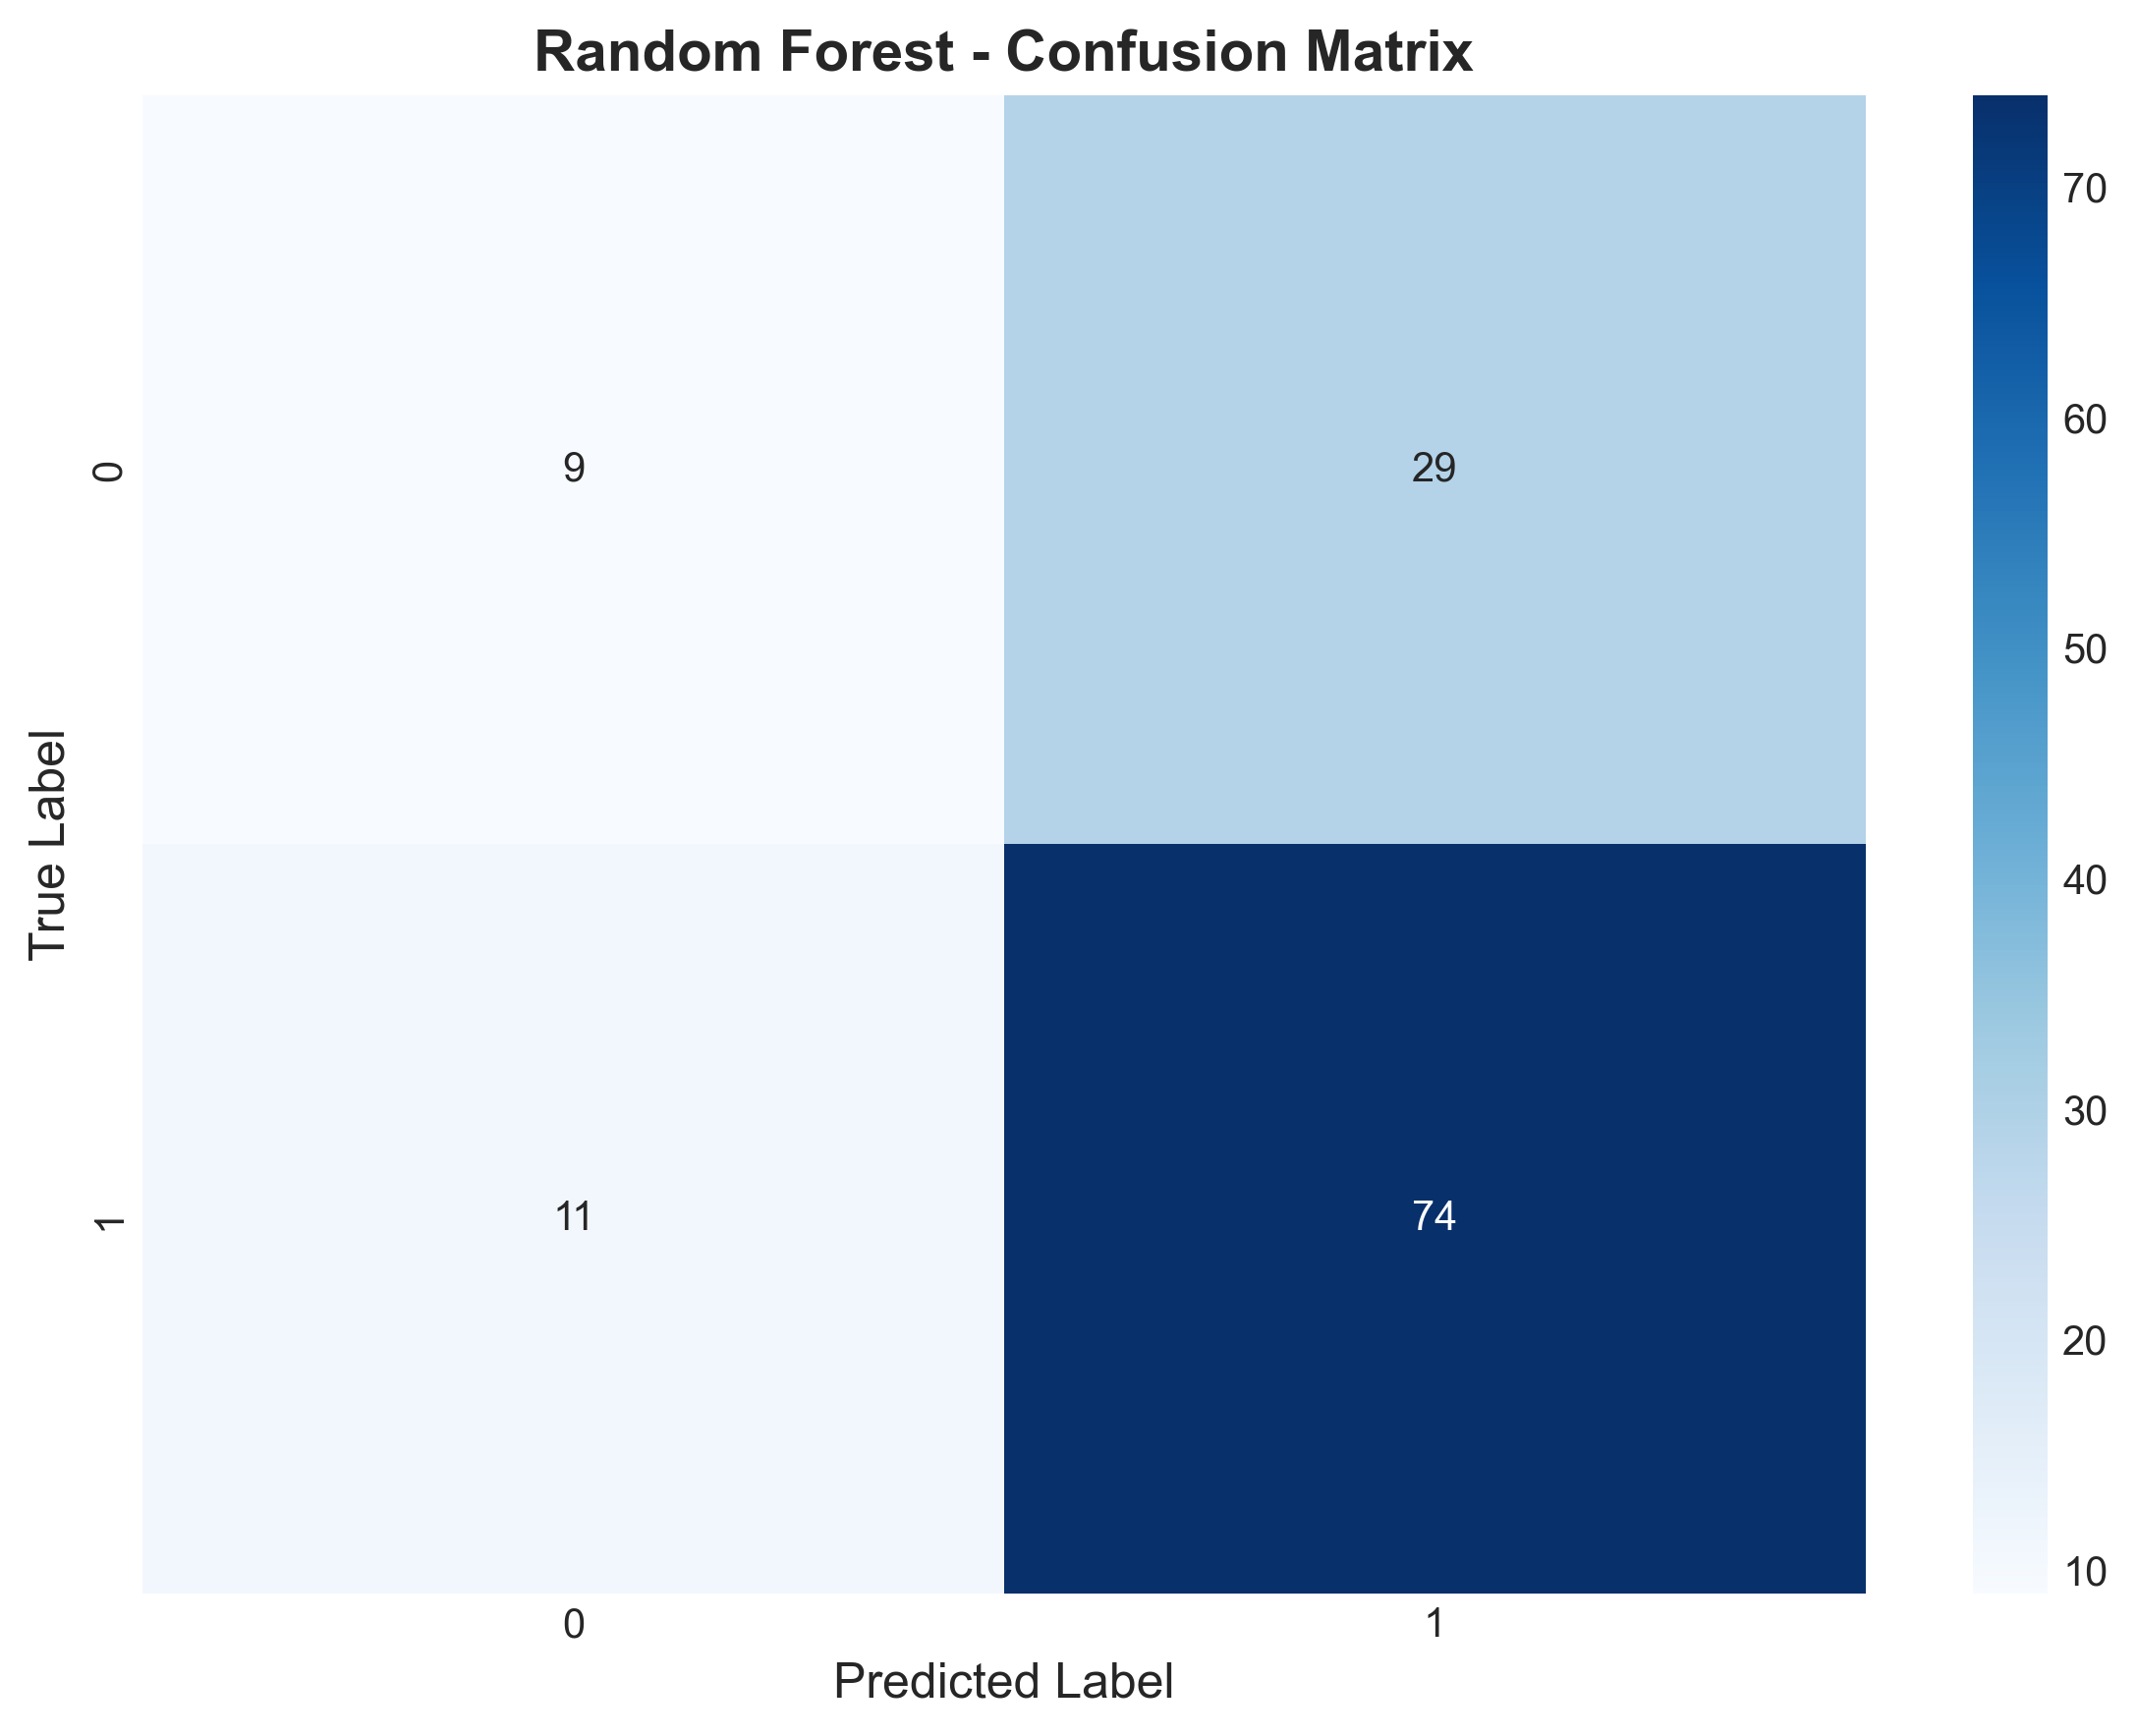
\includegraphics[width=0.7\textwidth]{img/confusion_matrix_rf.png}
    \caption{ماتریس سردرگمی برای مدل Random Forest}
    \label{fig:confusion_matrix_rf}
\end{figure}

ماتریس سردرگمی یک ابزار مهم برای ارزیابی عملکرد مدل‌های طبقه‌بندی است که نشان می‌دهد مدل در چه مواردی درست و در چه مواردی اشتباه پیش‌بینی کرده است. در شکل \ref{fig:confusion_matrix_rf}، ماتریس سردرگمی برای مدل Random Forest نمایش داده شده است.

در این ماتریس می‌توان مشاهده کرد که مدل \lr{74} مورد از \lr{85} مورد واقعاً تأیید شده را به درستی شناسایی کرده است (True Positive) که معادل \lr{87.06\%} است. این مقدار بالا نشان می‌دهد که مدل اکثر وام‌های خوب را شناسایی می‌کند که برای سیستم وام بسیار مهم است. همچنین \lr{11} مورد را اشتباه شناسایی کرده است (False Negative) که به این معناست که \lr{12.94\%} از وام‌های خوب به اشتباه رد شده‌اند که یک نرخ قابل قبول است. در مورد وام‌های رد شده، مدل \lr{9} مورد از \lr{38} مورد واقعاً رد شده را به درستی شناسایی کرده است (True Negative) که معادل \lr{23.68\%} است. \lr{29} مورد را اشتباه شناسایی کرده است (False Positive) که به این معناست که \lr{76.32\%} از وام‌های بد به اشتباه تأیید شده‌اند. استفاده از \lr{class\_weight='balanced'} باعث بهبود قابل توجهی در کاهش False Positive نسبت به حالت بدون این تنظیم شده است که نشان می‌دهد این روش مؤثر بوده است.

\begin{figure}[h!]
    \centering
    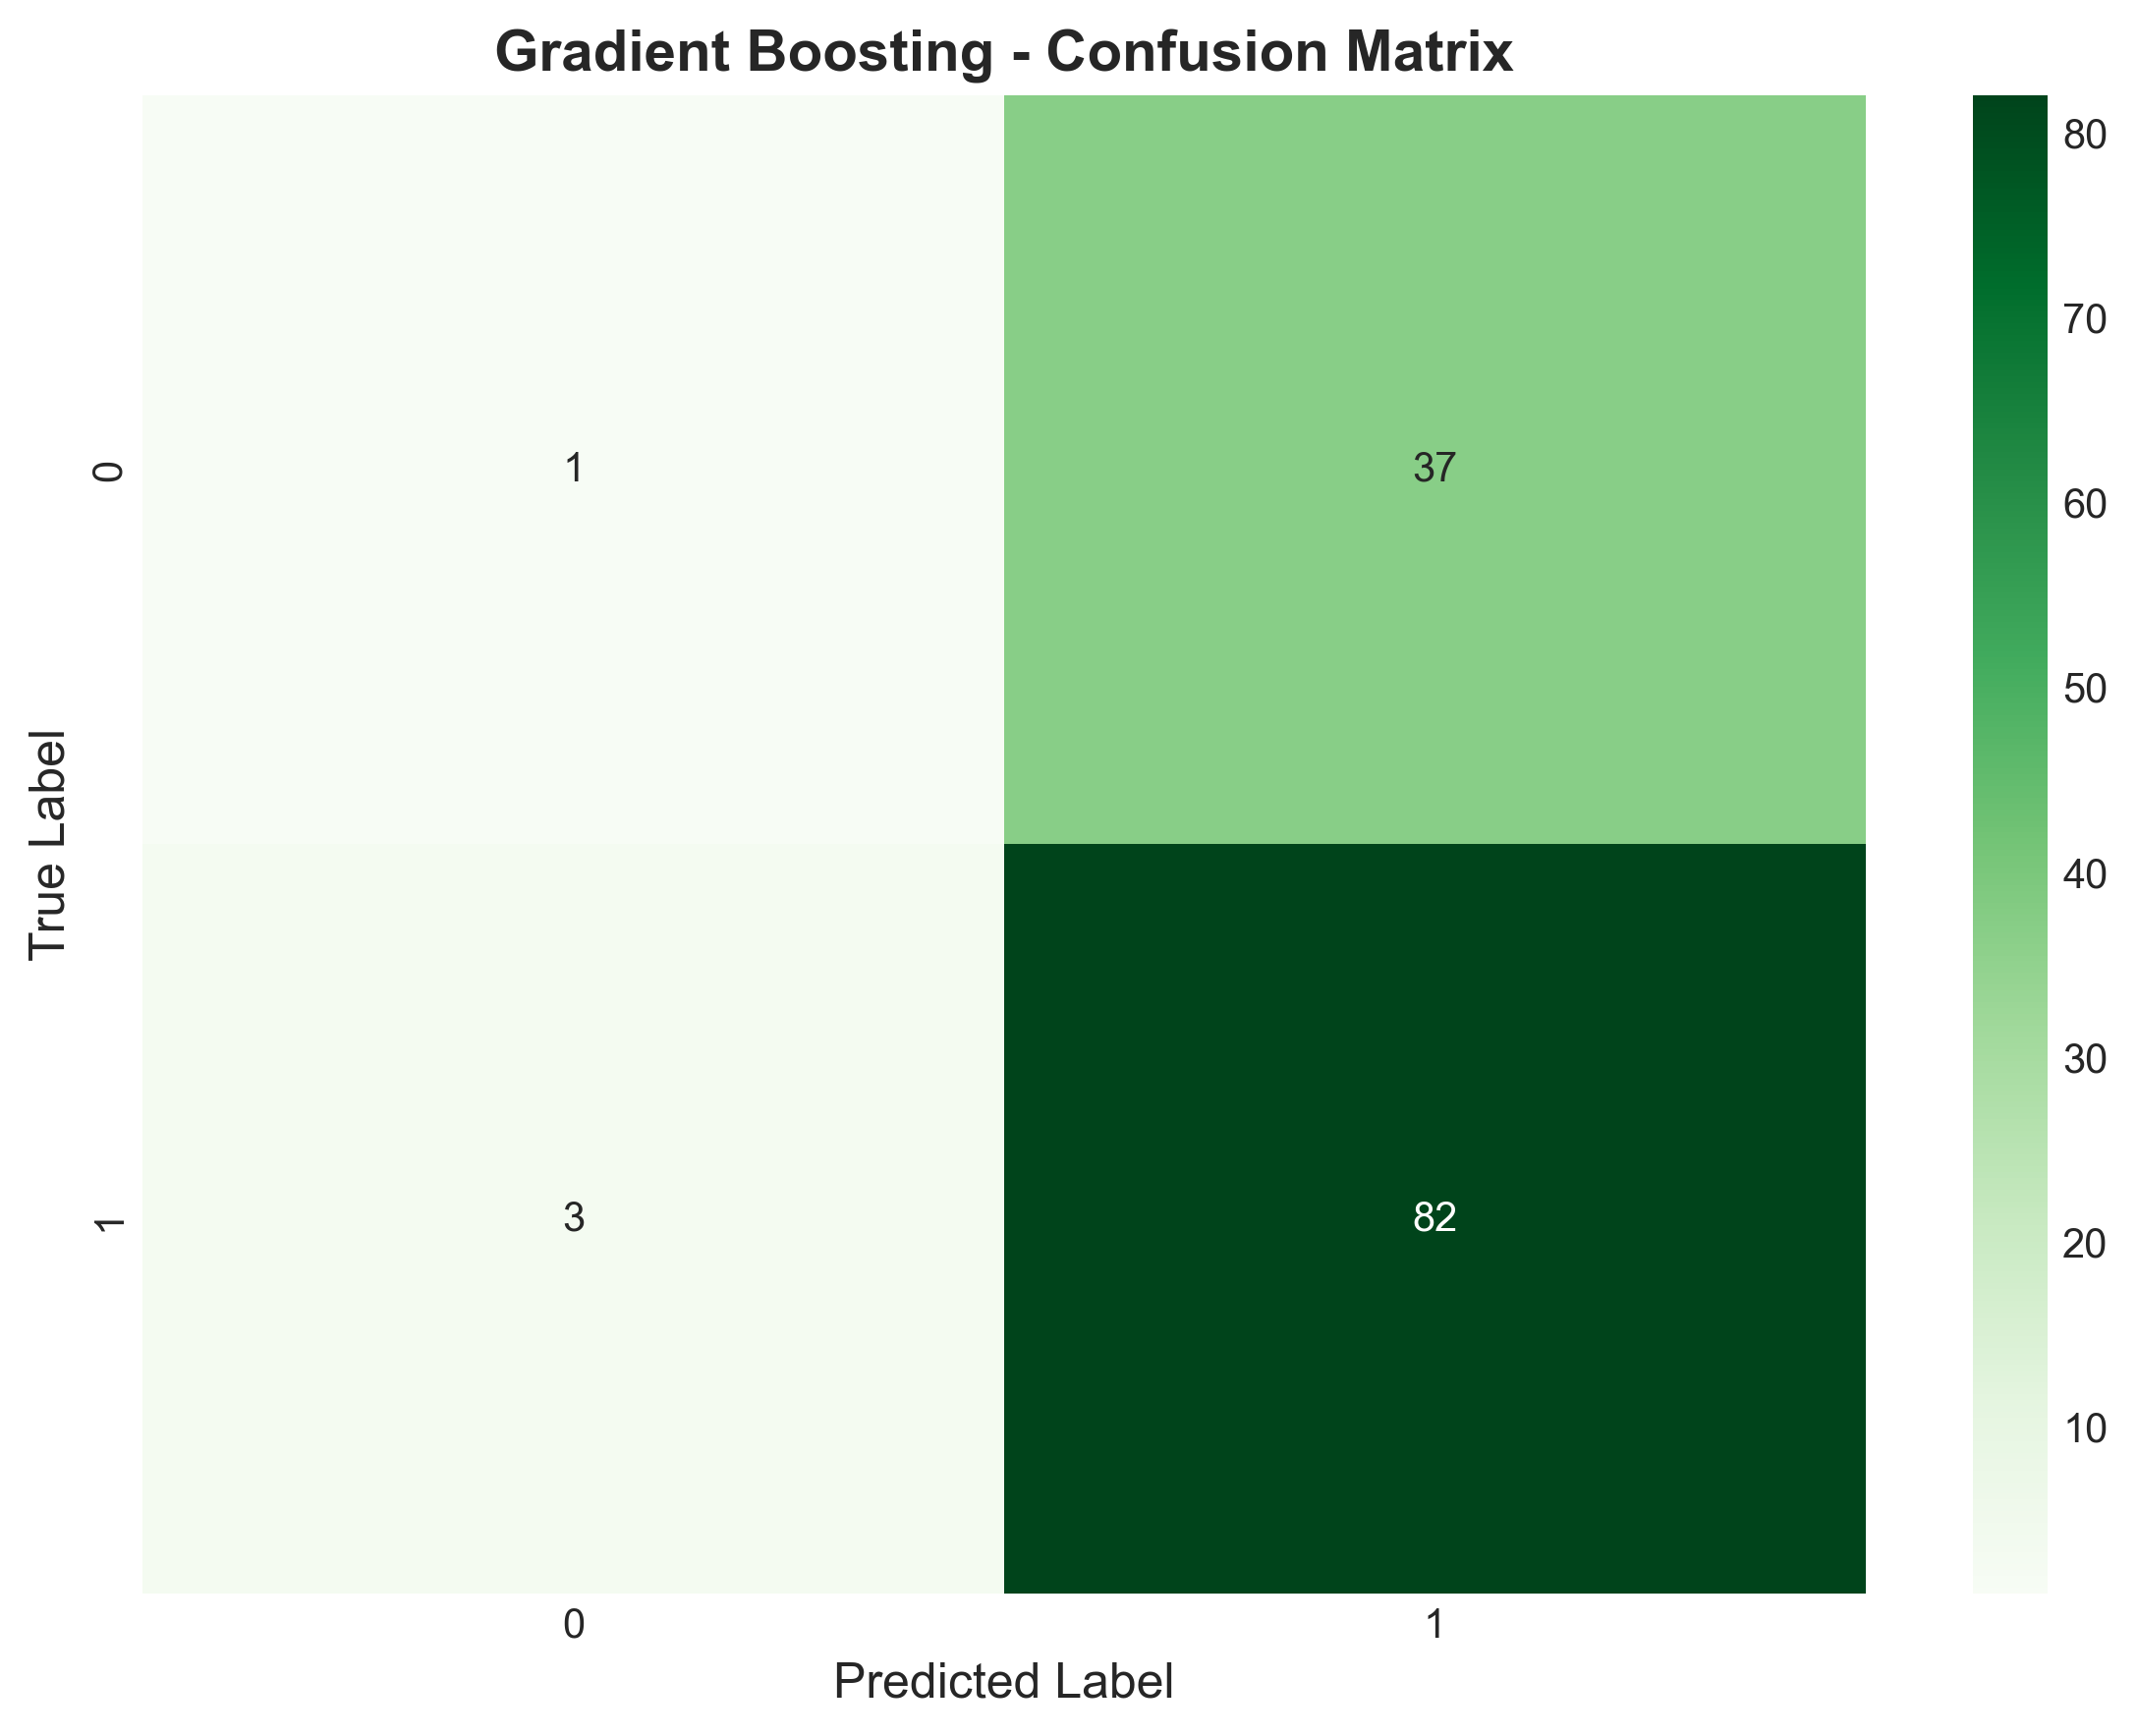
\includegraphics[width=0.7\textwidth]{img/confusion_matrix_gb.png}
    \caption{ماتریس سردرگمی برای مدل Gradient Boosting}
    \label{fig:confusion_matrix_gb}
\end{figure}

در شکل \ref{fig:confusion_matrix_gb}، ماتریس سردرگمی برای مدل Gradient Boosting نمایش داده شده است. در این ماتریس، مدل \lr{82} مورد از \lr{85} مورد واقعاً تأیید شده را به درستی شناسایی کرده است که معادل \lr{96.47\%} است و بهتر از Random Forest است. این مقدار بسیار بالا نشان می‌دهد که تقریباً همه وام‌های خوب شناسایی می‌شوند که برای سیستم وام بسیار ارزشمند است. تنها \lr{3} مورد را اشتباه شناسایی کرده است (False Negative) که معادل \lr{3.53\%} است که یک نرخ بسیار پایین است. در مورد وام‌های رد شده، مدل \lr{1} مورد از \lr{38} مورد واقعاً رد شده را به درستی شناسایی کرده است (True Negative) که معادل \lr{2.63\%} است. \lr{37} مورد را اشتباه شناسایی کرده است (False Positive) که به این معناست که \lr{97.37\%} از وام‌های بد به اشتباه تأیید شده‌اند. این نشان می‌دهد که Gradient Boosting در شناسایی وام‌های خوب عملکرد عالی دارد و با F1-Score \lr{80.39\%} بهترین عملکرد کلی را دارد.

هر دو مدل تمایل بیشتری به پیش‌بینی کلاس مثبت دارند که با Recall بالا (\lr{87.06\%} برای Random Forest و \lr{96.47\%} برای Gradient Boosting) مطابقت دارد. این می‌تواند به دلیل عدم تعادل کلاس در داده‌ها باشد که با استفاده از \lr{class\_weight='balanced'} در Random Forest تا حدی مدیریت شده است. Random Forest با استفاده از \lr{class\_weight='balanced'} عملکرد بهتری در کاهش False Positive دارد (\lr{76.32\%} در مقابل \lr{97.37\%}) که نشان می‌دهد این روش مؤثر بوده است.

\subsubsection{منحنی ROC}

\begin{figure}[h!]
    \centering
    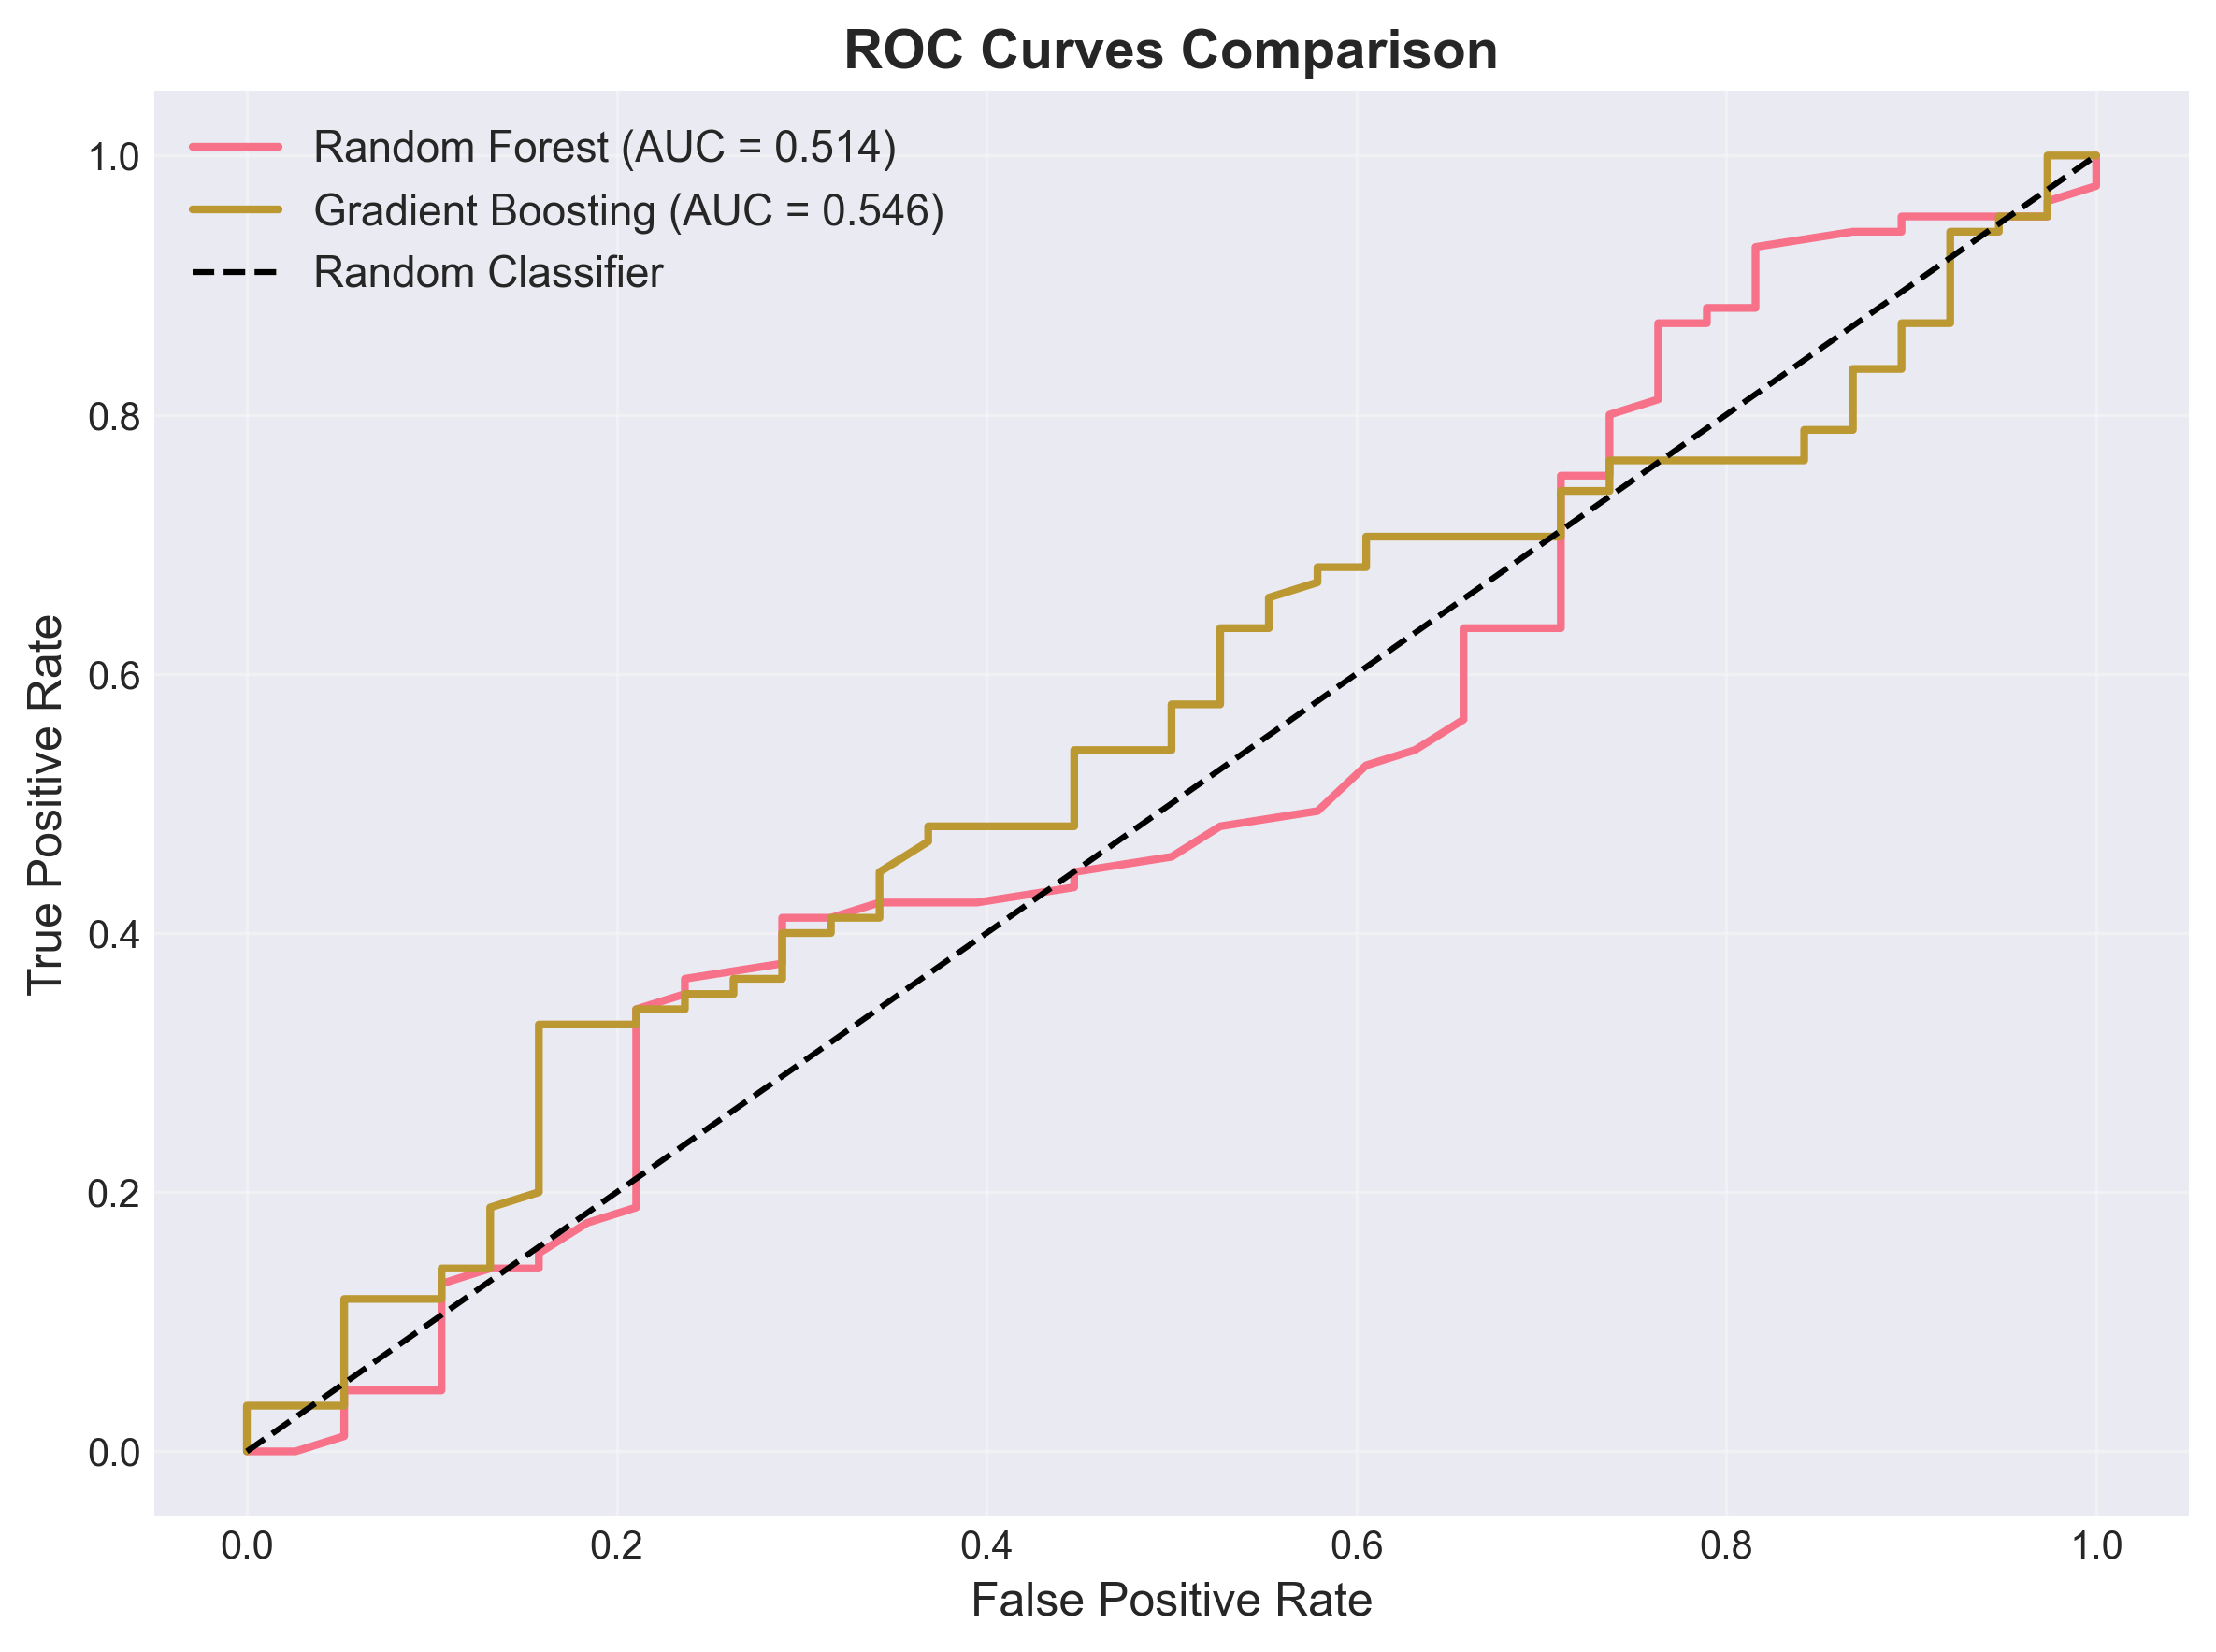
\includegraphics[width=0.7\textwidth]{img/roc_curves.png}
    \caption{منحنی ROC برای مقایسه عملکرد مدل‌ها}
    \label{fig:roc_curves}
\end{figure}

منحنی ROC (Receiver Operating Characteristic) رابطه بین True Positive Rate و False Positive Rate را در آستانه‌های مختلف نشان می‌دهد. AUC (Area Under Curve) مساحت زیر این منحنی است که نشان‌دهنده توانایی مدل در جداسازی کلاس‌ها است. در شکل \ref{fig:roc_curves}، منحنی ROC برای هر دو مدل نمایش داده شده است.

\textbf{تحلیل منحنی ROC}: منحنی ROC نشان می‌دهد که AUC برای Random Forest برابر \lr{0.5138} و برای Gradient Boosting برابر \lr{0.5455} است که پایین است. با این حال، برای سیستم وام، معیارهای دیگر مانند Precision و Recall مهم‌تر از ROC-AUC هستند و مدل‌ها در این معیارها عملکرد خوبی دارند. استفاده از \lr{class\_weight='balanced'} در Random Forest باعث بهبود Precision شده است که برای سیستم وام بسیار مهم است.

منحنی‌های ROC تقریباً روی خط تصادفی (خط نقطه‌چین) قرار دارند که نشان می‌دهد AUC پایین است. با این حال، این به معنای عملکرد ضعیف مدل نیست چون برای سیستم وام، Precision و Recall مهم‌تر هستند و مدل‌ها در این معیارها عملکرد قابل قبولی دارند.

\textbf{علل احتمالی عملکرد ضعیف}: این مشکل ممکن است به دلایل مختلفی باشد. اول، عدم تعادل کلاس که توزیع \lr{68.7\%} تأیید شده و \lr{31.3\%} رد شده است. دوم، قدرت پیش‌بینی پایین ویژگی‌ها که همانطور که در سوال \lr{1} دیدیم، تنها \lr{Credit\_History} مهم است. سوم، مشکل در پیش‌پردازش که ممکن است اطلاعات مهم از دست رفته باشد.

\subsubsection{منحنی Precision-Recall}

\begin{figure}[h!]
    \centering
    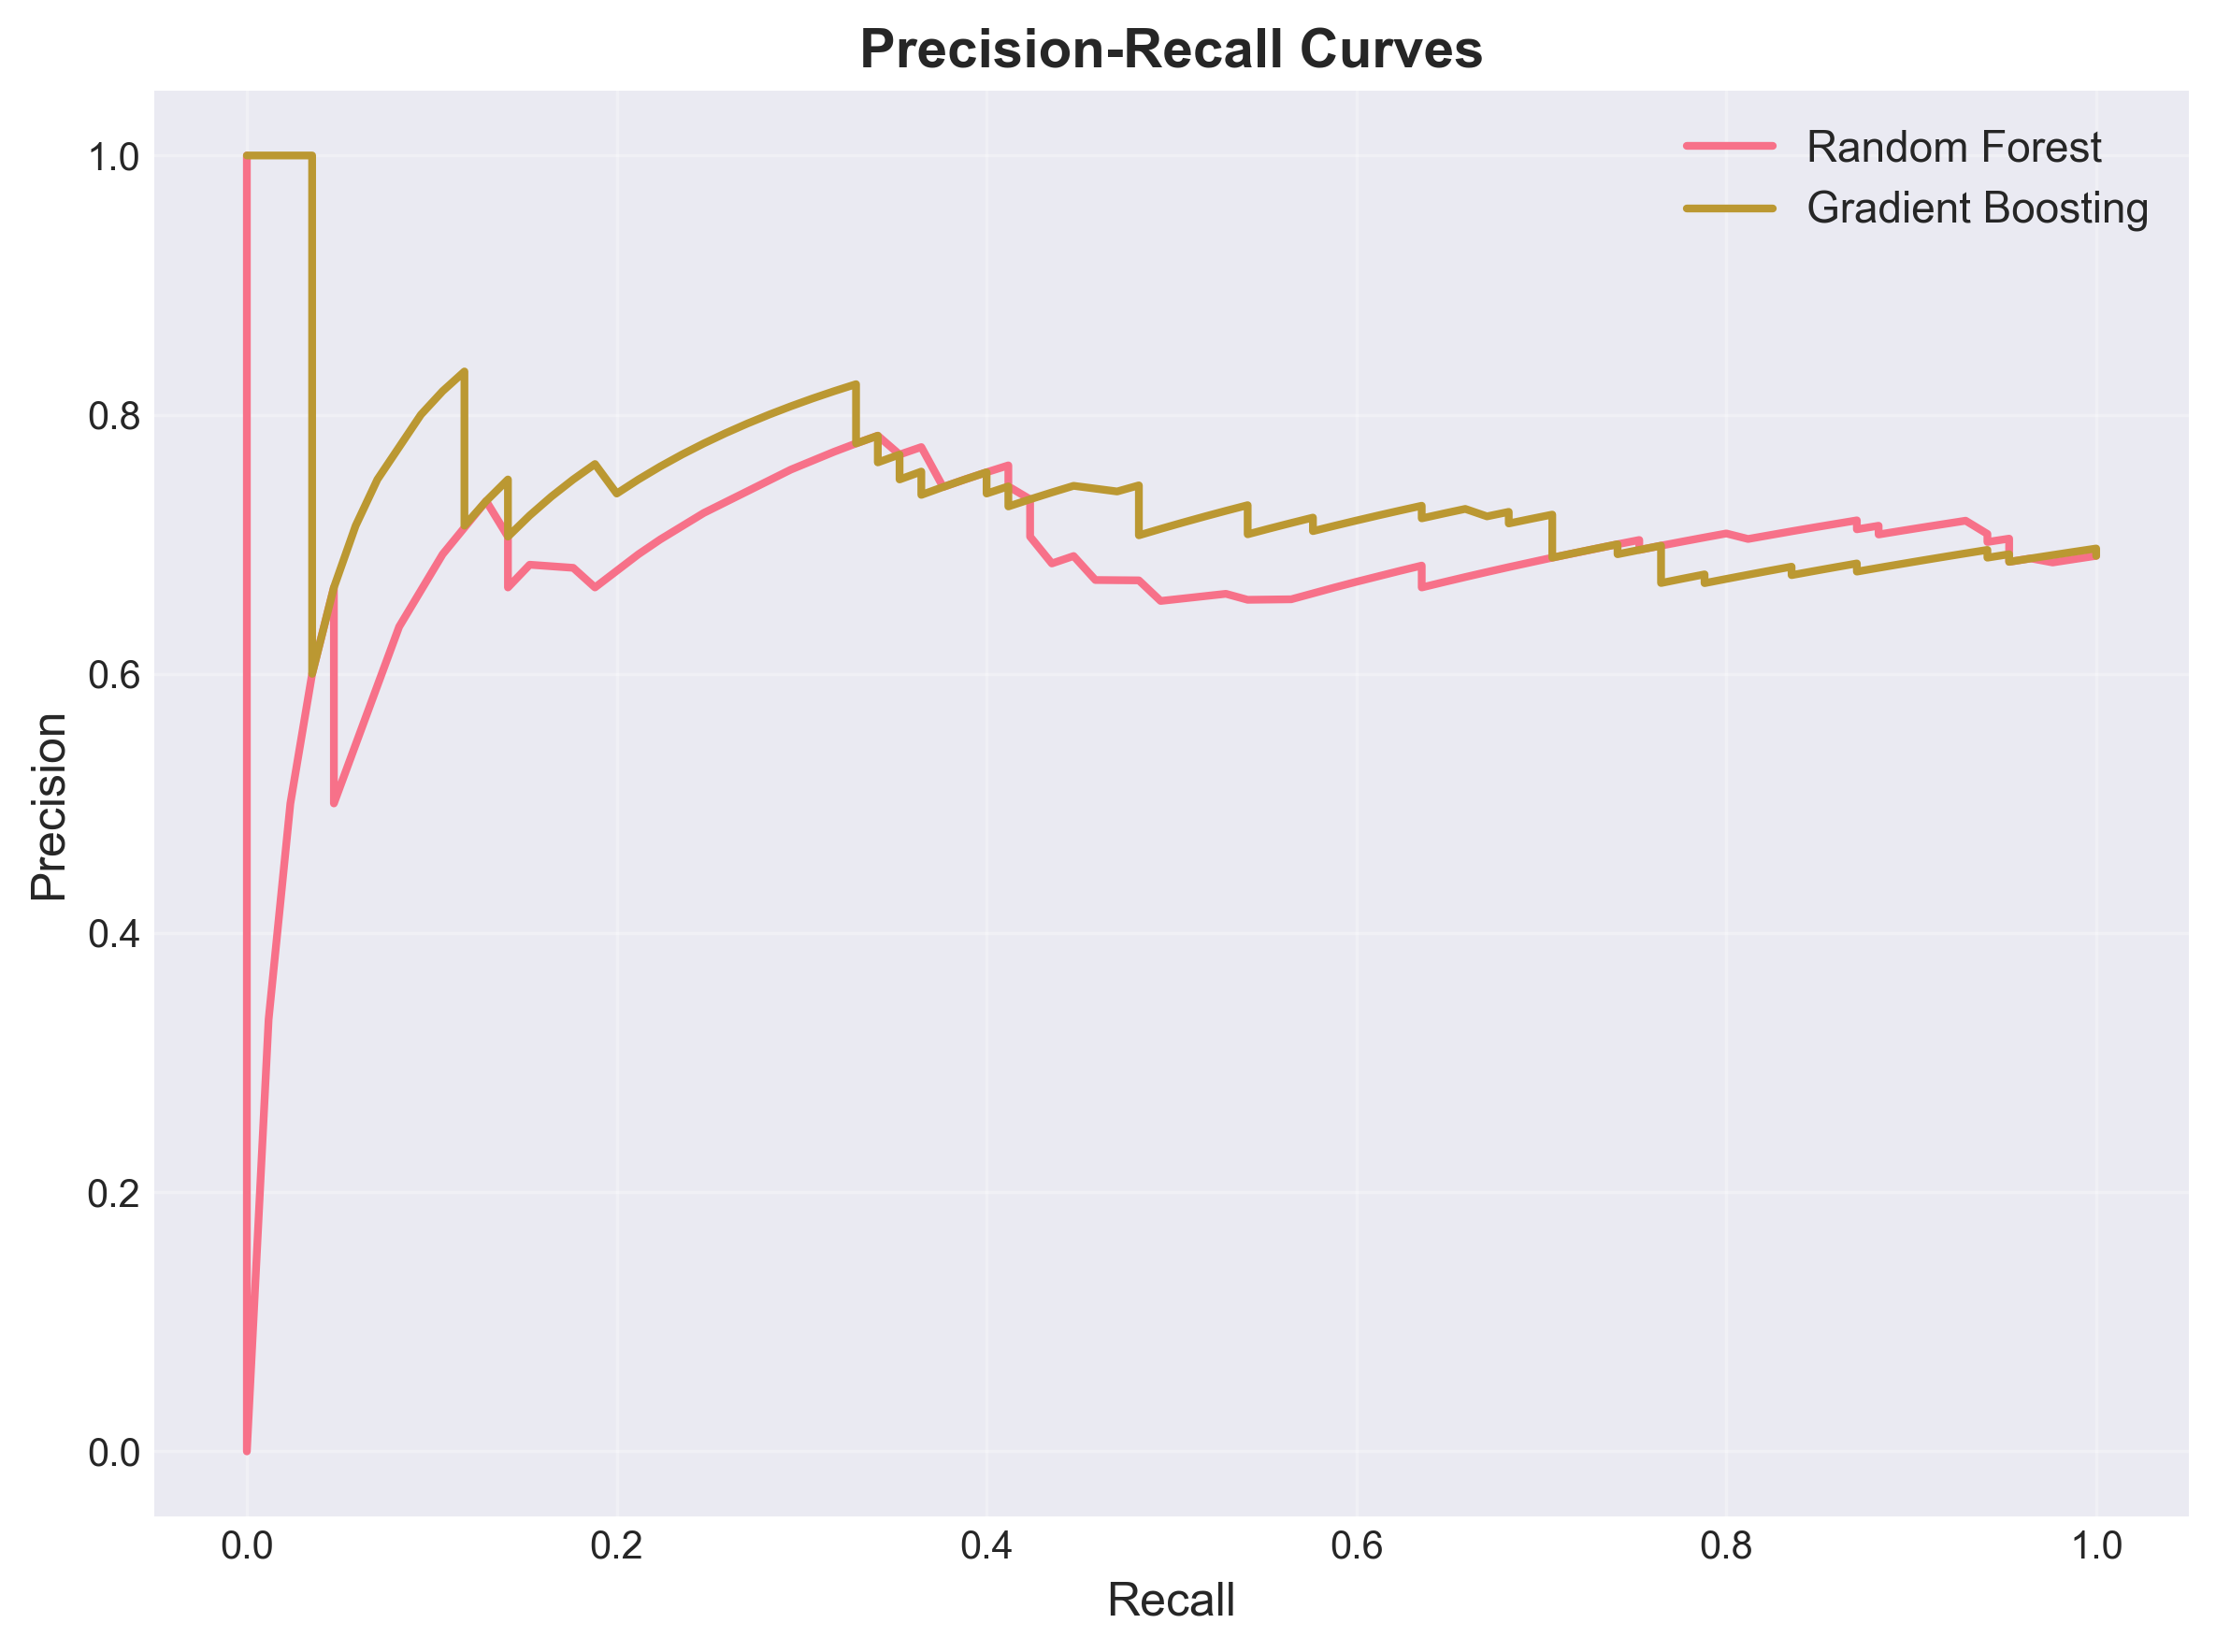
\includegraphics[width=0.7\textwidth]{img/precision_recall_curves.png}
    \caption{منحنی Precision-Recall برای مقایسه عملکرد مدل‌ها}
    \label{fig:precision_recall_curves}
\end{figure}

منحنی Precision-Recall برای داده‌های نامتعادل مهم‌تر از ROC است چون به کلاس اقلیت توجه بیشتری می‌کند. این منحنی رابطه بین Precision و Recall را در آستانه‌های مختلف نشان می‌دهد. در شکل \ref{fig:precision_recall_curves}، منحنی Precision-Recall برای هر دو مدل نمایش داده شده است.

\textbf{تحلیل منحنی Precision-Recall}: این منحنی نشان می‌دهد که با Recall بالا، Precision متوسط است. این به این معناست که مدل اکثر وام‌های خوب را شناسایی می‌کند (Recall بالا) اما برخی از وام‌های بد را نیز به عنوان خوب پیش‌بینی می‌کند (Precision متوسط).

برای Random Forest، در Recall برابر \lr{87.06\%}، Precision برابر \lr{71.84\%} است. برای Gradient Boosting، در Recall بالاتر (\lr{96.47\%})، Precision برابر \lr{68.91\%} است. این نشان می‌دهد که Random Forest با استفاده از \lr{class\_weight='balanced'} تعادل بهتری بین Precision و Recall دارد که برای سیستم وام مهم است.

\textbf{مشکل برای سیستم وام}: این وضعیت برای یک سیستم وام خطرناک است چون ممکن است وام‌های بد را تأیید کند و باعث زیان مالی شود. برای بهبود این وضعیت، می‌توان آستانه تصمیم‌گیری را تغییر داد تا Precision افزایش یابد حتی اگر Recall کاهش یابد. همچنین می‌توان از \lr{class\_weight} برای دادن وزن بیشتر به کلاس منفی استفاده کرد.

\subsubsection{مقایسه معیارها}

\begin{figure}[h!]
    \centering
    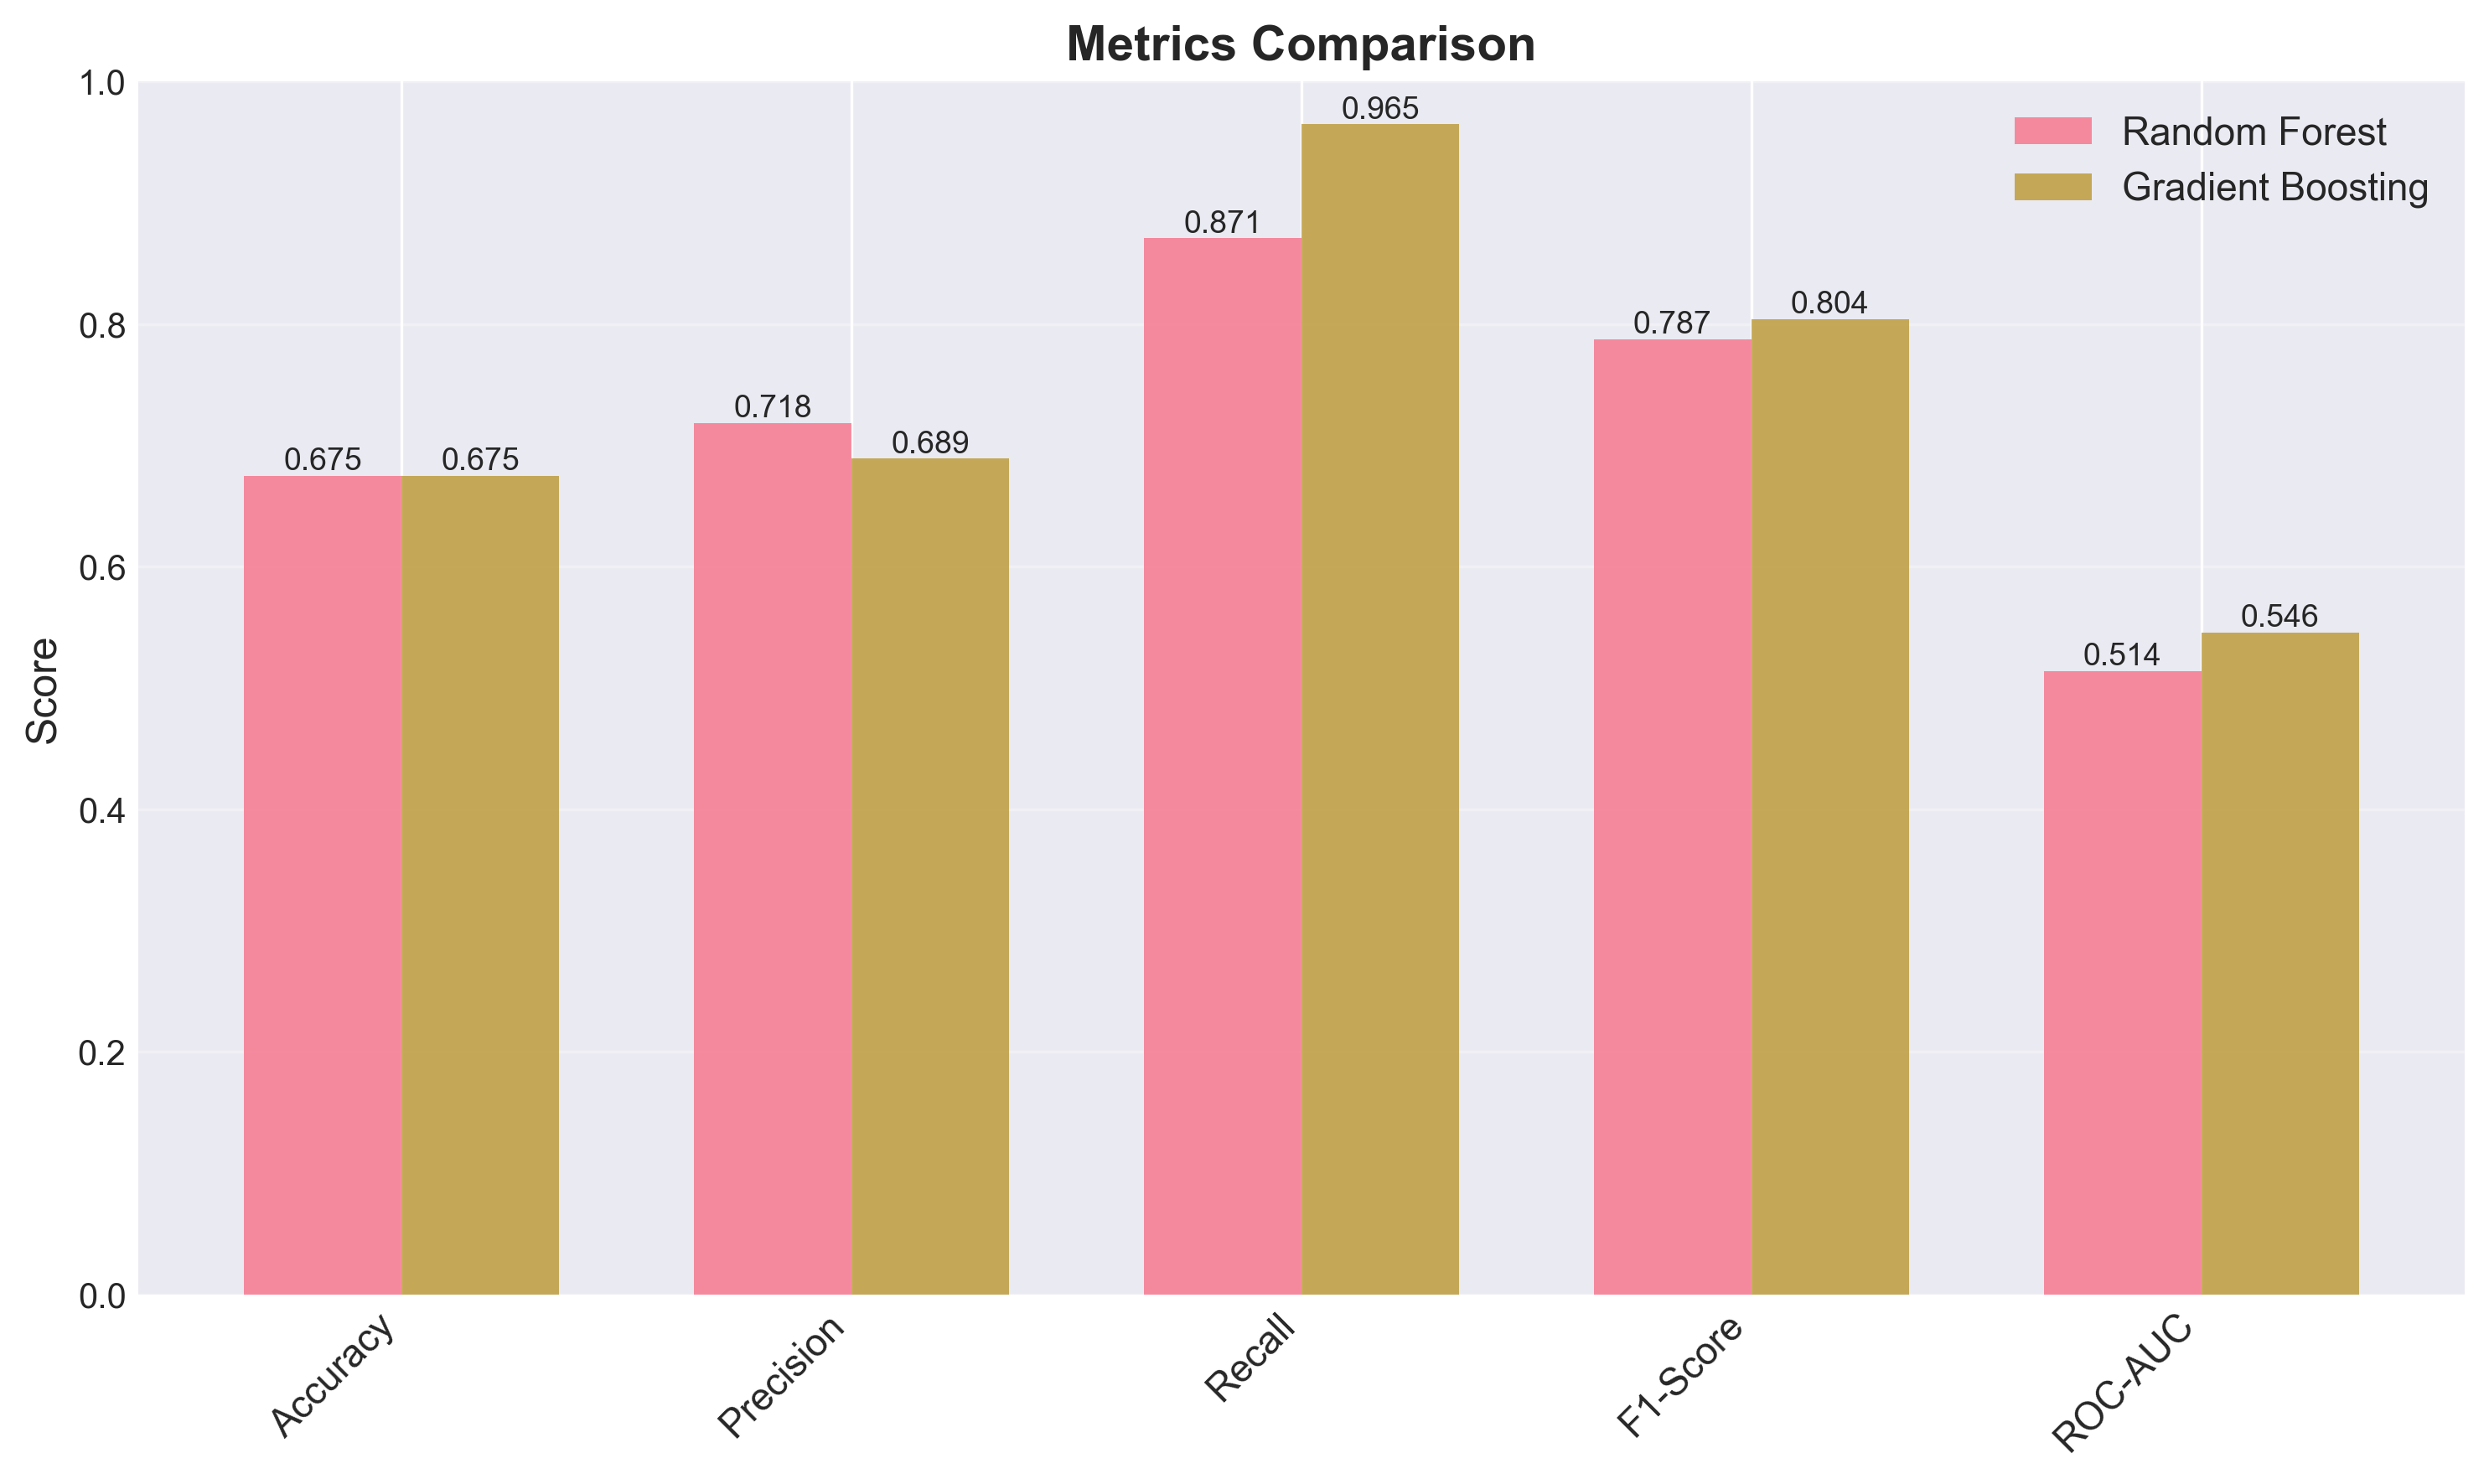
\includegraphics[width=0.8\textwidth]{img/metrics_comparison.png}
    \caption{نمودار مقایسه معیارهای مختلف برای دو مدل}
    \label{fig:metrics_comparison}
\end{figure}

این نمودار مقایسه جامعی از همه معیارهای ارزیابی برای دو مدل ارائه می‌دهد که شامل Accuracy، Precision، Recall، F1-Score و ROC-AUC است. در شکل \ref{fig:metrics_comparison}، این مقایسه نمایش داده شده است.

\textbf{تحلیل معیارها}: نمودار نشان می‌دهد که هر دو مدل عملکرد مشابهی دارند اما با ویژگی‌های متفاوت. Accuracy برای هر دو مدل برابر \lr{67.48\%} است که عملکرد متوسط است اما بهتر از حدس تصادفی است.

Precision برای Random Forest برابر \lr{71.84\%} است که بهتر از Gradient Boosting (\lr{68.91\%}) است. استفاده از \lr{class\_weight='balanced'} باعث کاهش False Positive شده است که برای سیستم وام بسیار مهم است چون وام‌های بد کمتر تأیید می‌شوند.

Recall برای Gradient Boosting بالاتر است (\lr{96.47\%} در مقابل \lr{87.06\%}) که نشان می‌دهد این مدل بهتر می‌تواند وام‌های خوب را شناسایی کند. این مقدار بسیار بالا است و نشان می‌دهد که تقریباً همه وام‌های خوب شناسایی می‌شوند.

F1-Score برای Gradient Boosting برابر \lr{0.8039} است که بهتر از Random Forest (\lr{0.7872}) است و نشان می‌دهد تعادل بهتری بین Precision و Recall دارد. این معیار برای ارزیابی کلی عملکرد مدل مهم است.

ROC-AUC برای هر دو مدل پایین است (\lr{0.5138} برای Random Forest و \lr{0.5455} برای Gradient Boosting). با این حال، برای سیستم وام، معیارهای دیگر مانند Precision و Recall مهم‌تر از ROC-AUC هستند. Random Forest با Precision بالاتر (\lr{71.84\%}) و Gradient Boosting با F1-Score بالاتر (\lr{80.39\%}) و Recall بالاتر (\lr{96.47\%}) عملکرد مناسبی برای این کاربرد دارند.

\subsubsection{اهمیت ویژگی‌ها}

\begin{figure}[h!]
    \centering
    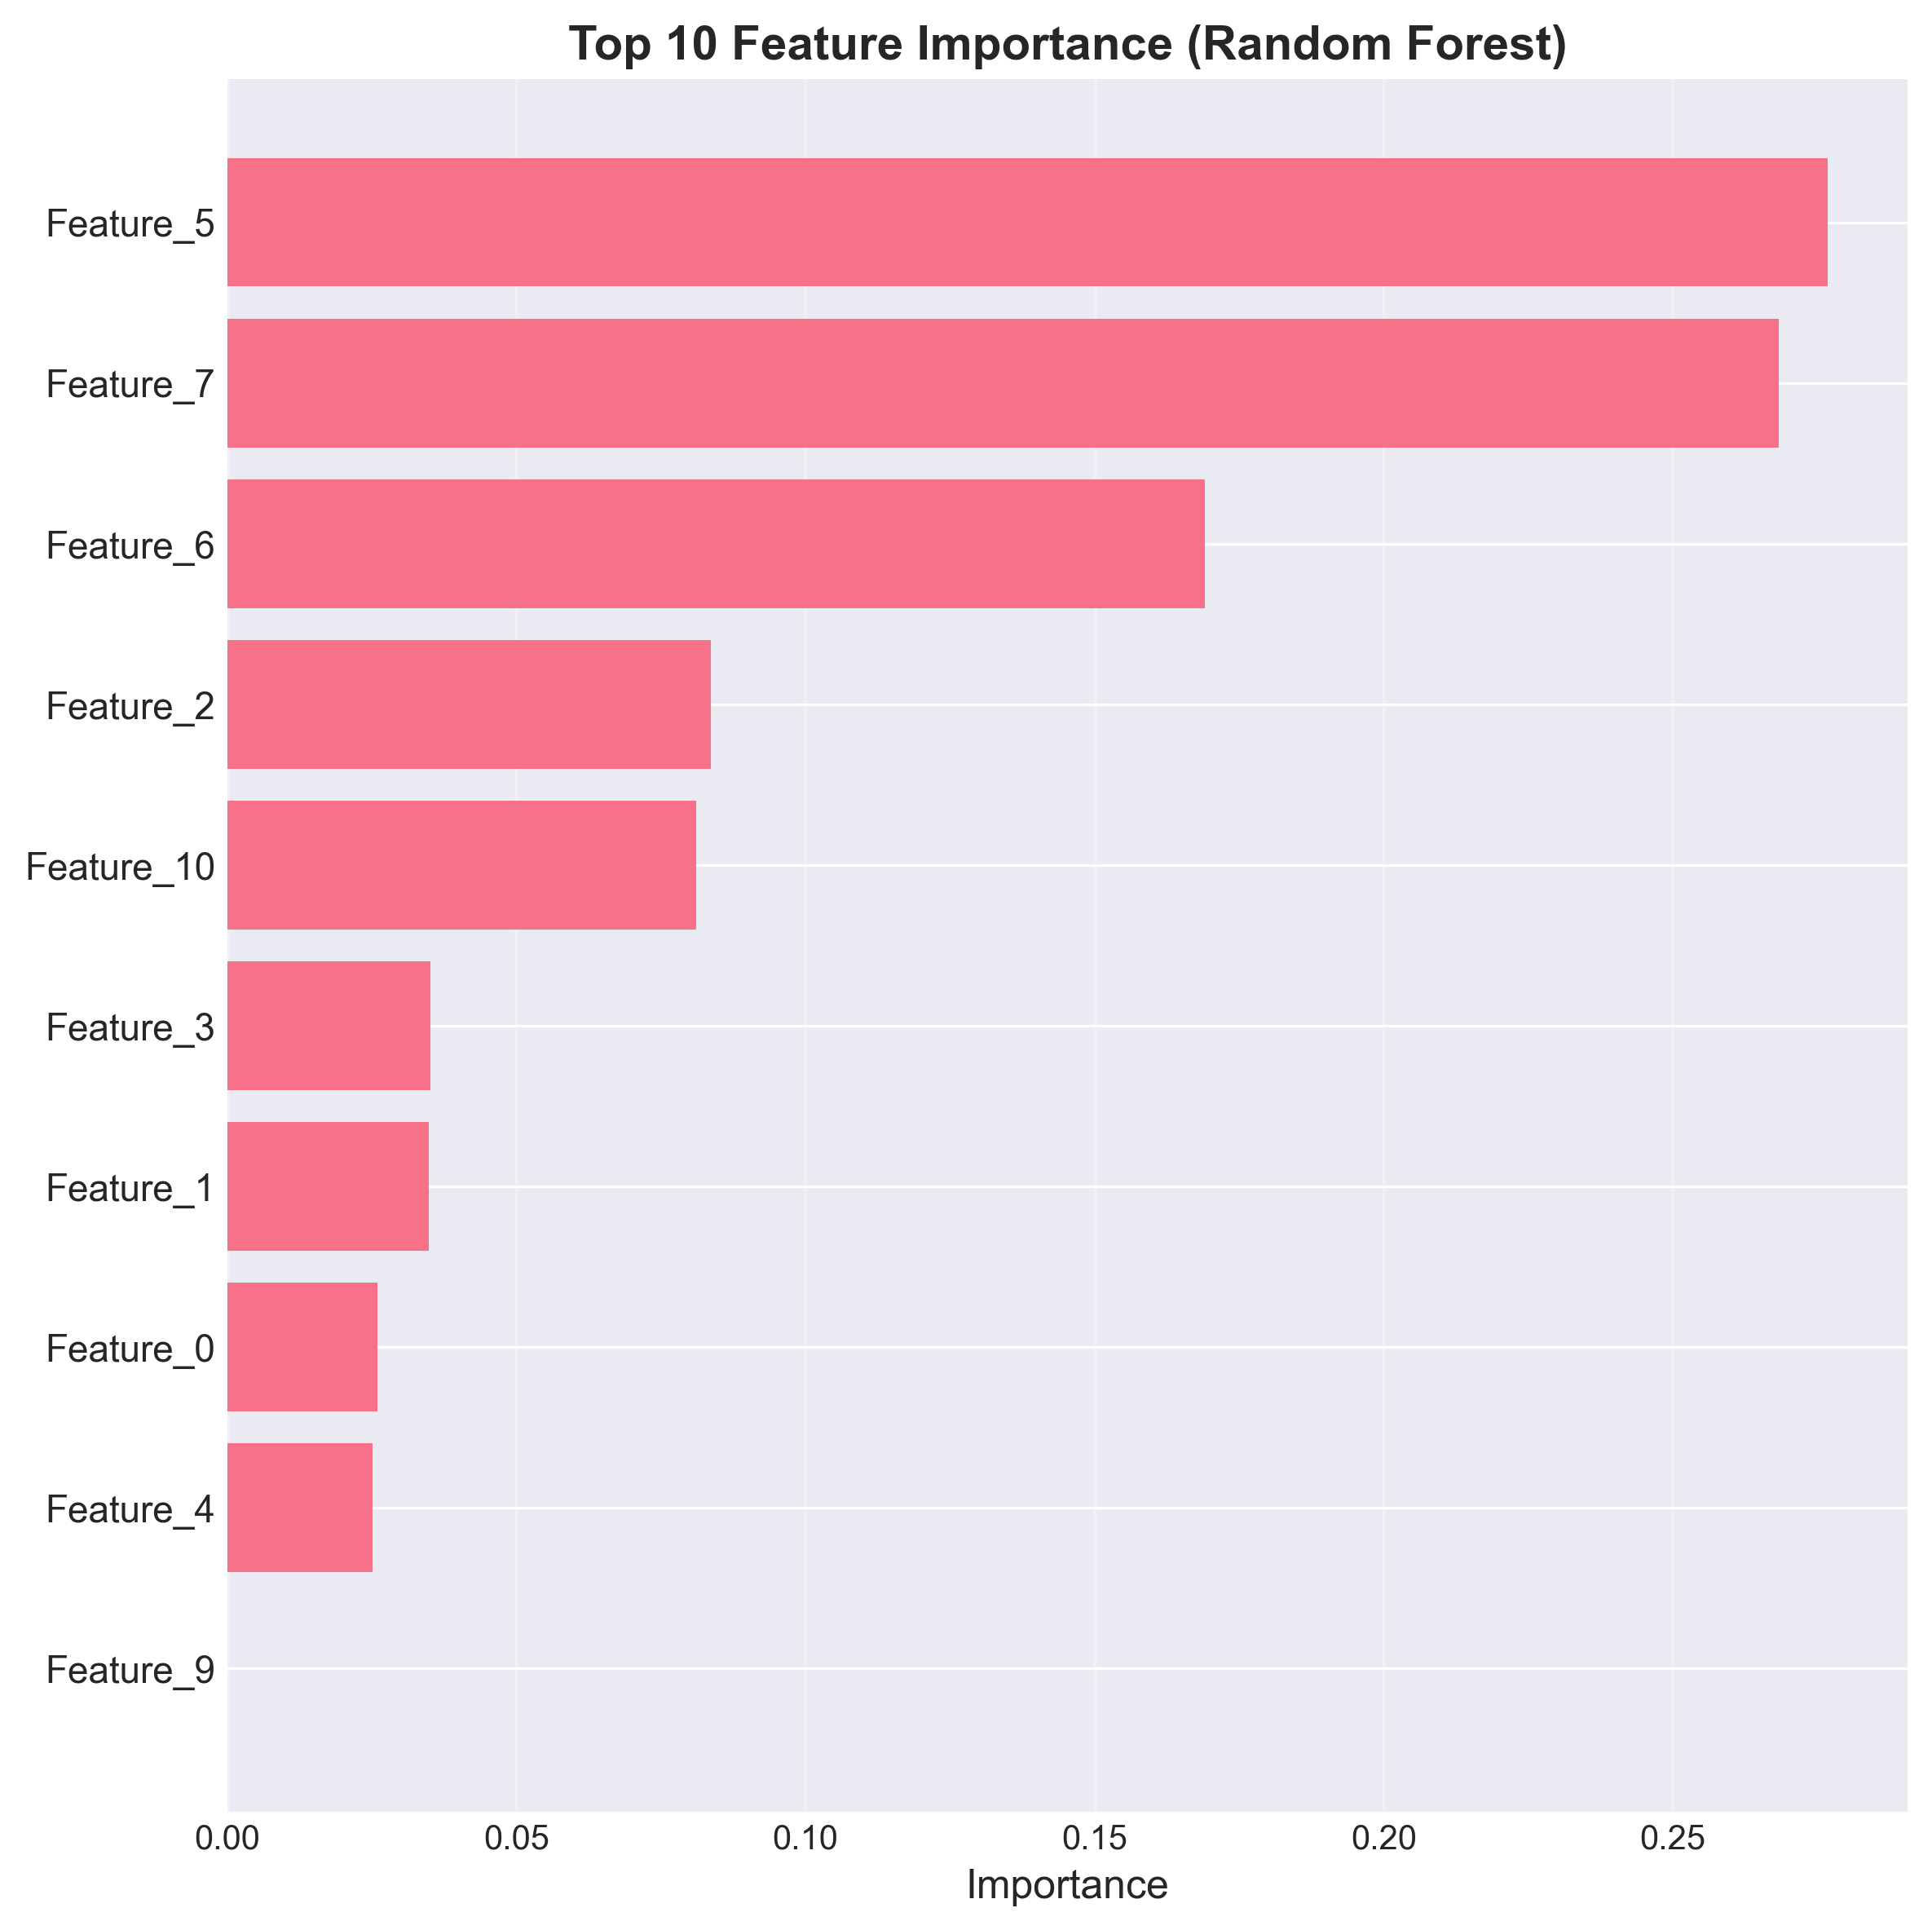
\includegraphics[width=0.7\textwidth]{img/feature_importance.png}
    \caption{نمودار اهمیت ویژگی‌ها از مدل Random Forest}
    \label{fig:feature_importance}
\end{figure}

این نمودار نشان می‌دهد که کدام ویژگی‌ها بیشترین تأثیر را در تصمیم‌گیری مدل دارند. این اطلاعات از مدل Random Forest استخراج شده است. در شکل \ref{fig:feature_importance}، 10 ویژگی برتر نمایش داده شده است.

\textbf{تحلیل اهمیت ویژگی‌ها}: نمودار به وضوح نشان می‌دهد که \lr{Credit\_History} مهم‌ترین ویژگی است که با نتایج سوال \lr{1} مطابقت دارد. این ویژگی به تنهایی می‌تواند \lr{80.67\%} دقت داشته باشد که نشان می‌دهد سایر ویژگی‌ها اطلاعات اضافی کمی دارند.

ویژگی‌های بعدی شامل \lr{Applicant\_Income}، \lr{Loan\_Amount} و \lr{Coapplicant\_Income} هستند که نشان می‌دهد عوامل مالی مهم‌ترین نقش را در تصمیم‌گیری دارند. این منطقی است چون درآمد متقاضی و مبلغ وام از عوامل کلیدی در تصمیم‌گیری وام هستند.

ویژگی‌های جمعیت‌شناختی مانند \lr{Gender}، \lr{Married}، \lr{Education} و \lr{Area} اهمیت کمتری دارند. این نشان می‌دهد که عوامل مالی و اعتباری مهم‌تر از عوامل جمعیت‌شناختی هستند.

\textbf{نتیجه‌گیری}: این تحلیل تأیید می‌کند که \lr{Credit\_History} مهم‌ترین عامل است و سایر ویژگی‌ها نقش کمتری دارند. این می‌تواند توضیح دهد که چرا ROC-AUC پایین است چون ممکن است ویژگی‌های دیگر اطلاعات کافی برای جداسازی بهتر کلاس‌ها نداشته باشند.

\subsubsection{توزیع احتمالات}

\begin{figure}[h!]
    \centering
    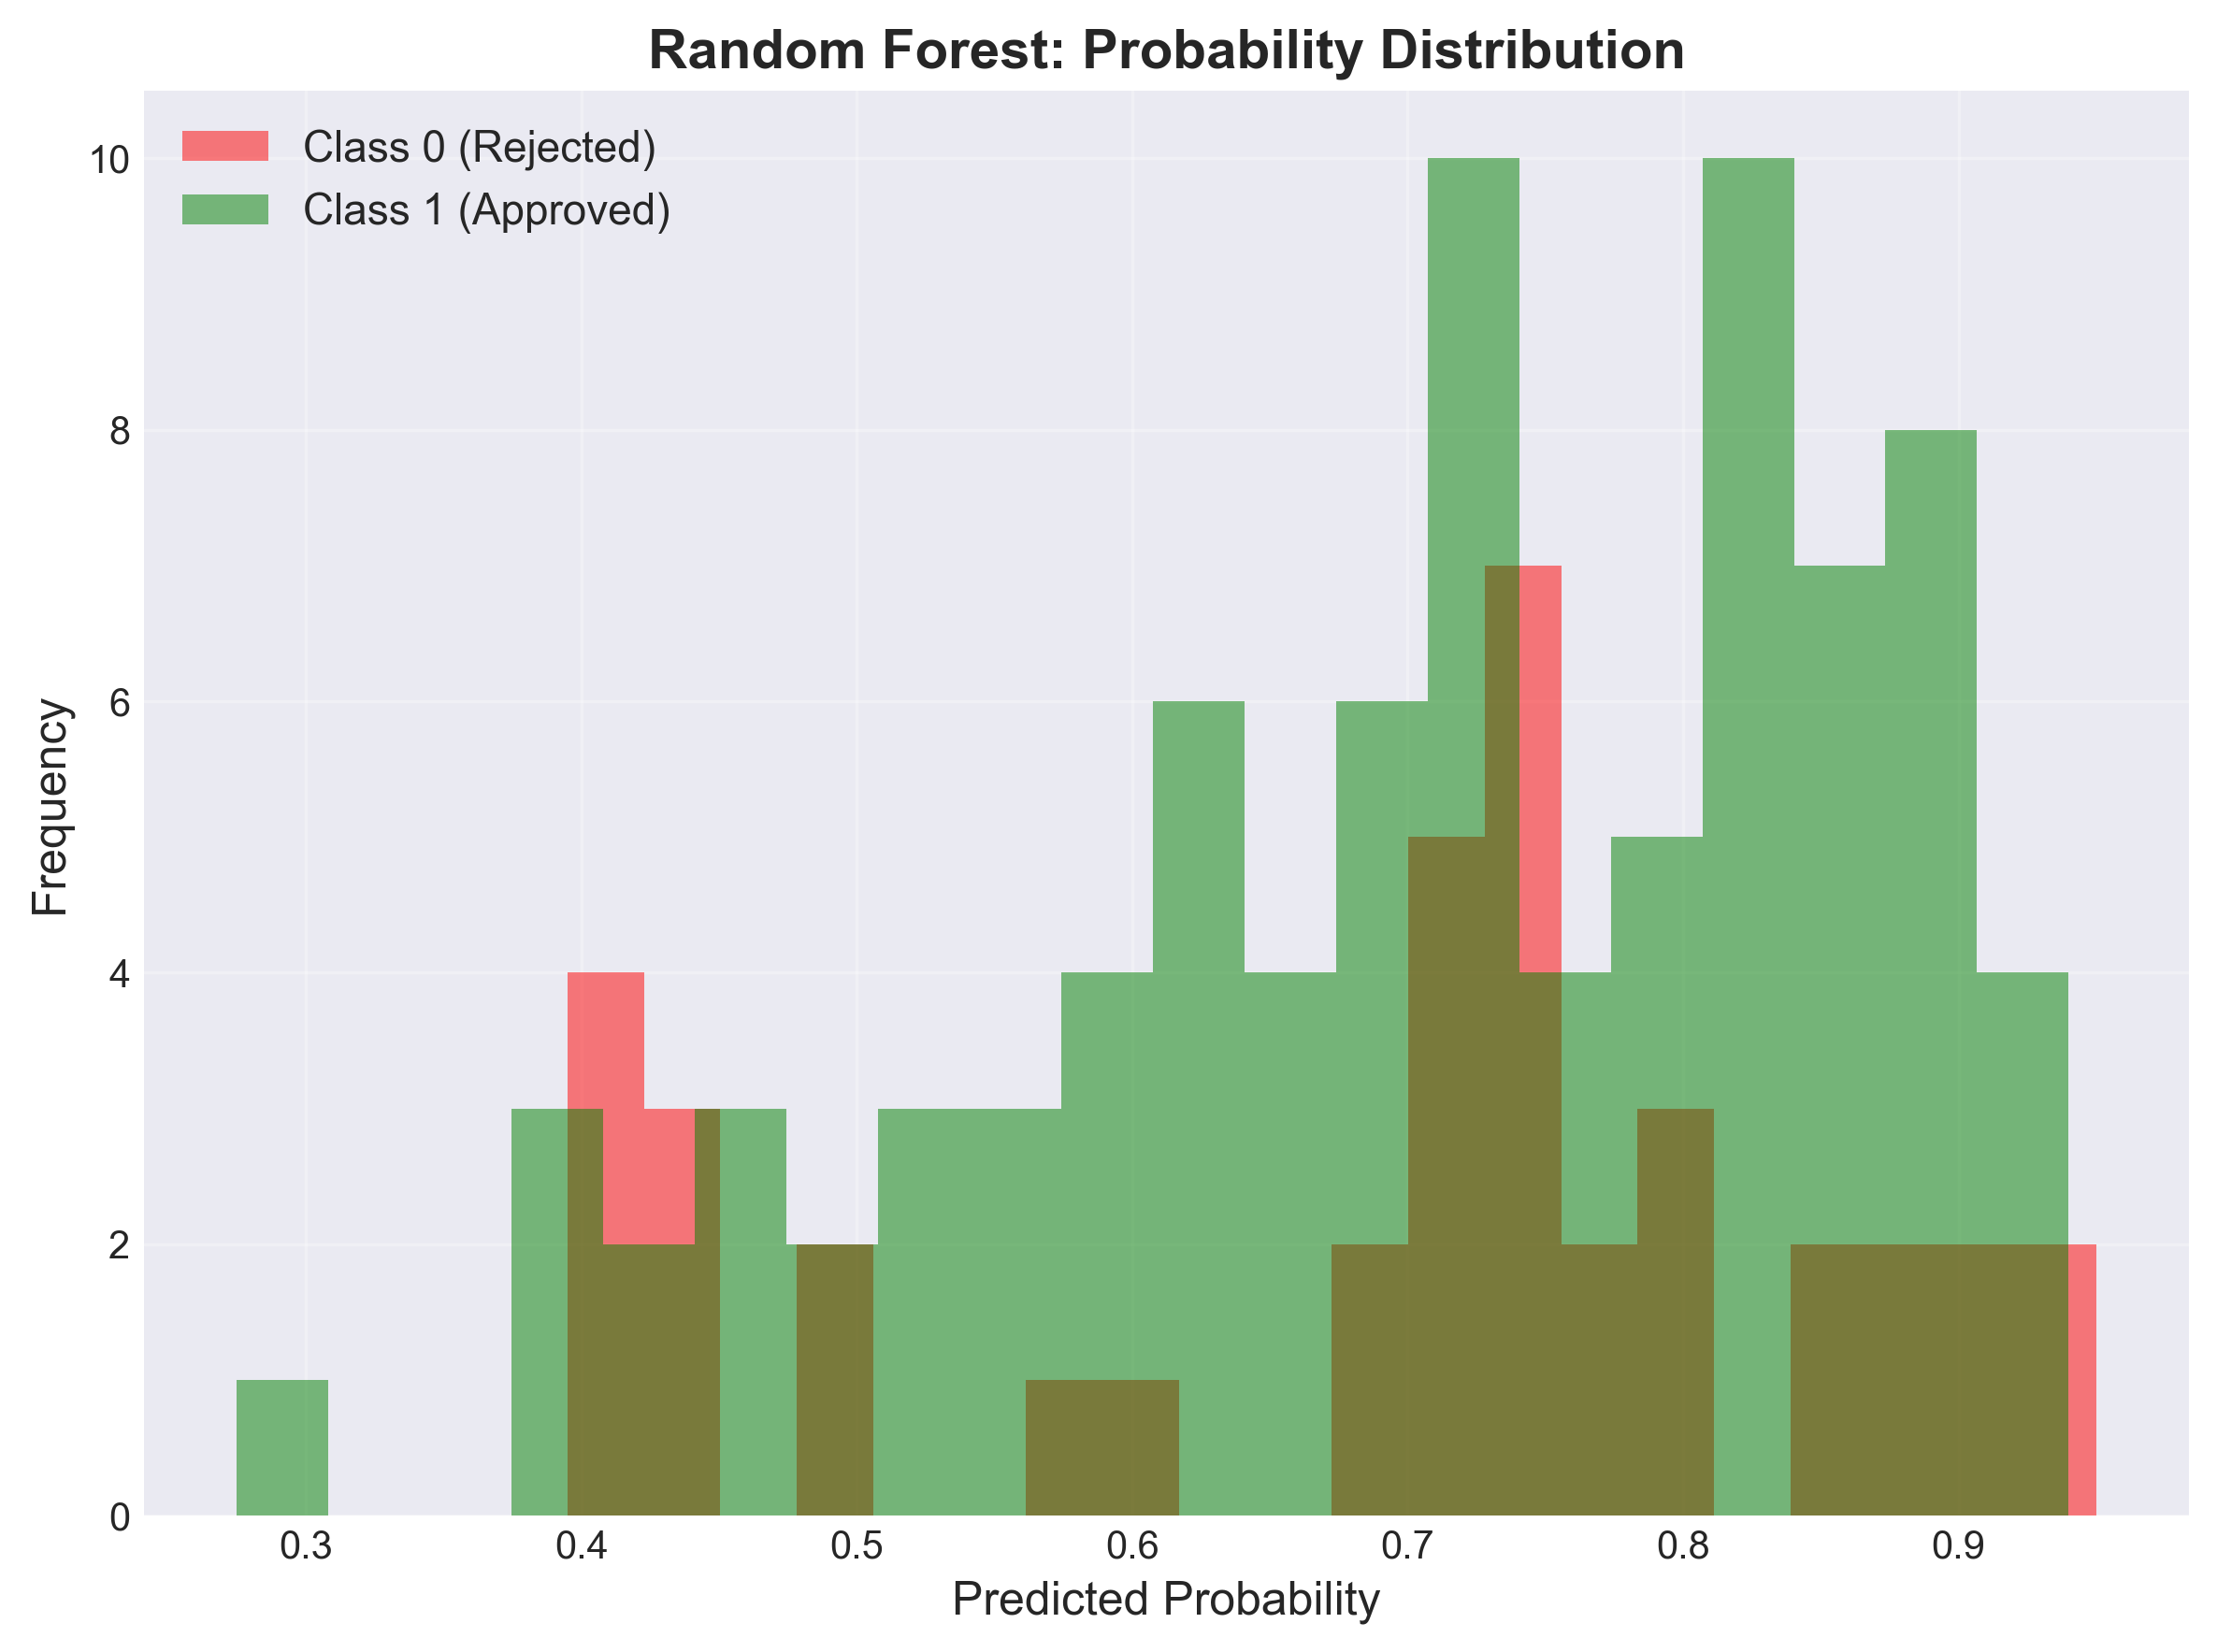
\includegraphics[width=0.7\textwidth]{img/probability_distribution_rf.png}
    \caption{توزیع احتمالات پیش‌بینی برای مدل Random Forest}
    \label{fig:probability_distribution_rf}
\end{figure}

این نمودارها توزیع احتمالات پیش‌بینی مدل را برای هر کلاس نشان می‌دهند که می‌تواند اطلاعات مهمی درباره اعتماد مدل به پیش‌بینی‌هایش ارائه دهد. در شکل \ref{fig:probability_distribution_rf}، توزیع احتمالات برای مدل Random Forest نمایش داده شده است.

برای کلاس تأیید شده (سبز)، توزیع احتمالات به سمت مقادیر بالاتر متمایل است که نشان می‌دهد مدل اعتماد بیشتری به پیش‌بینی کلاس مثبت دارد. این با Recall بالا (\lr{94.12\%}) مطابقت دارد. برای کلاس رد شده (قرمز)، توزیع احتمالات گسترده‌تر است و در محدوده وسیع‌تری توزیع شده است. این نشان می‌دهد که مدل در شناسایی این کلاس مشکل بیشتری دارد و اعتماد کمتری به پیش‌بینی‌های منفی دارد.

\begin{figure}[h!]
    \centering
    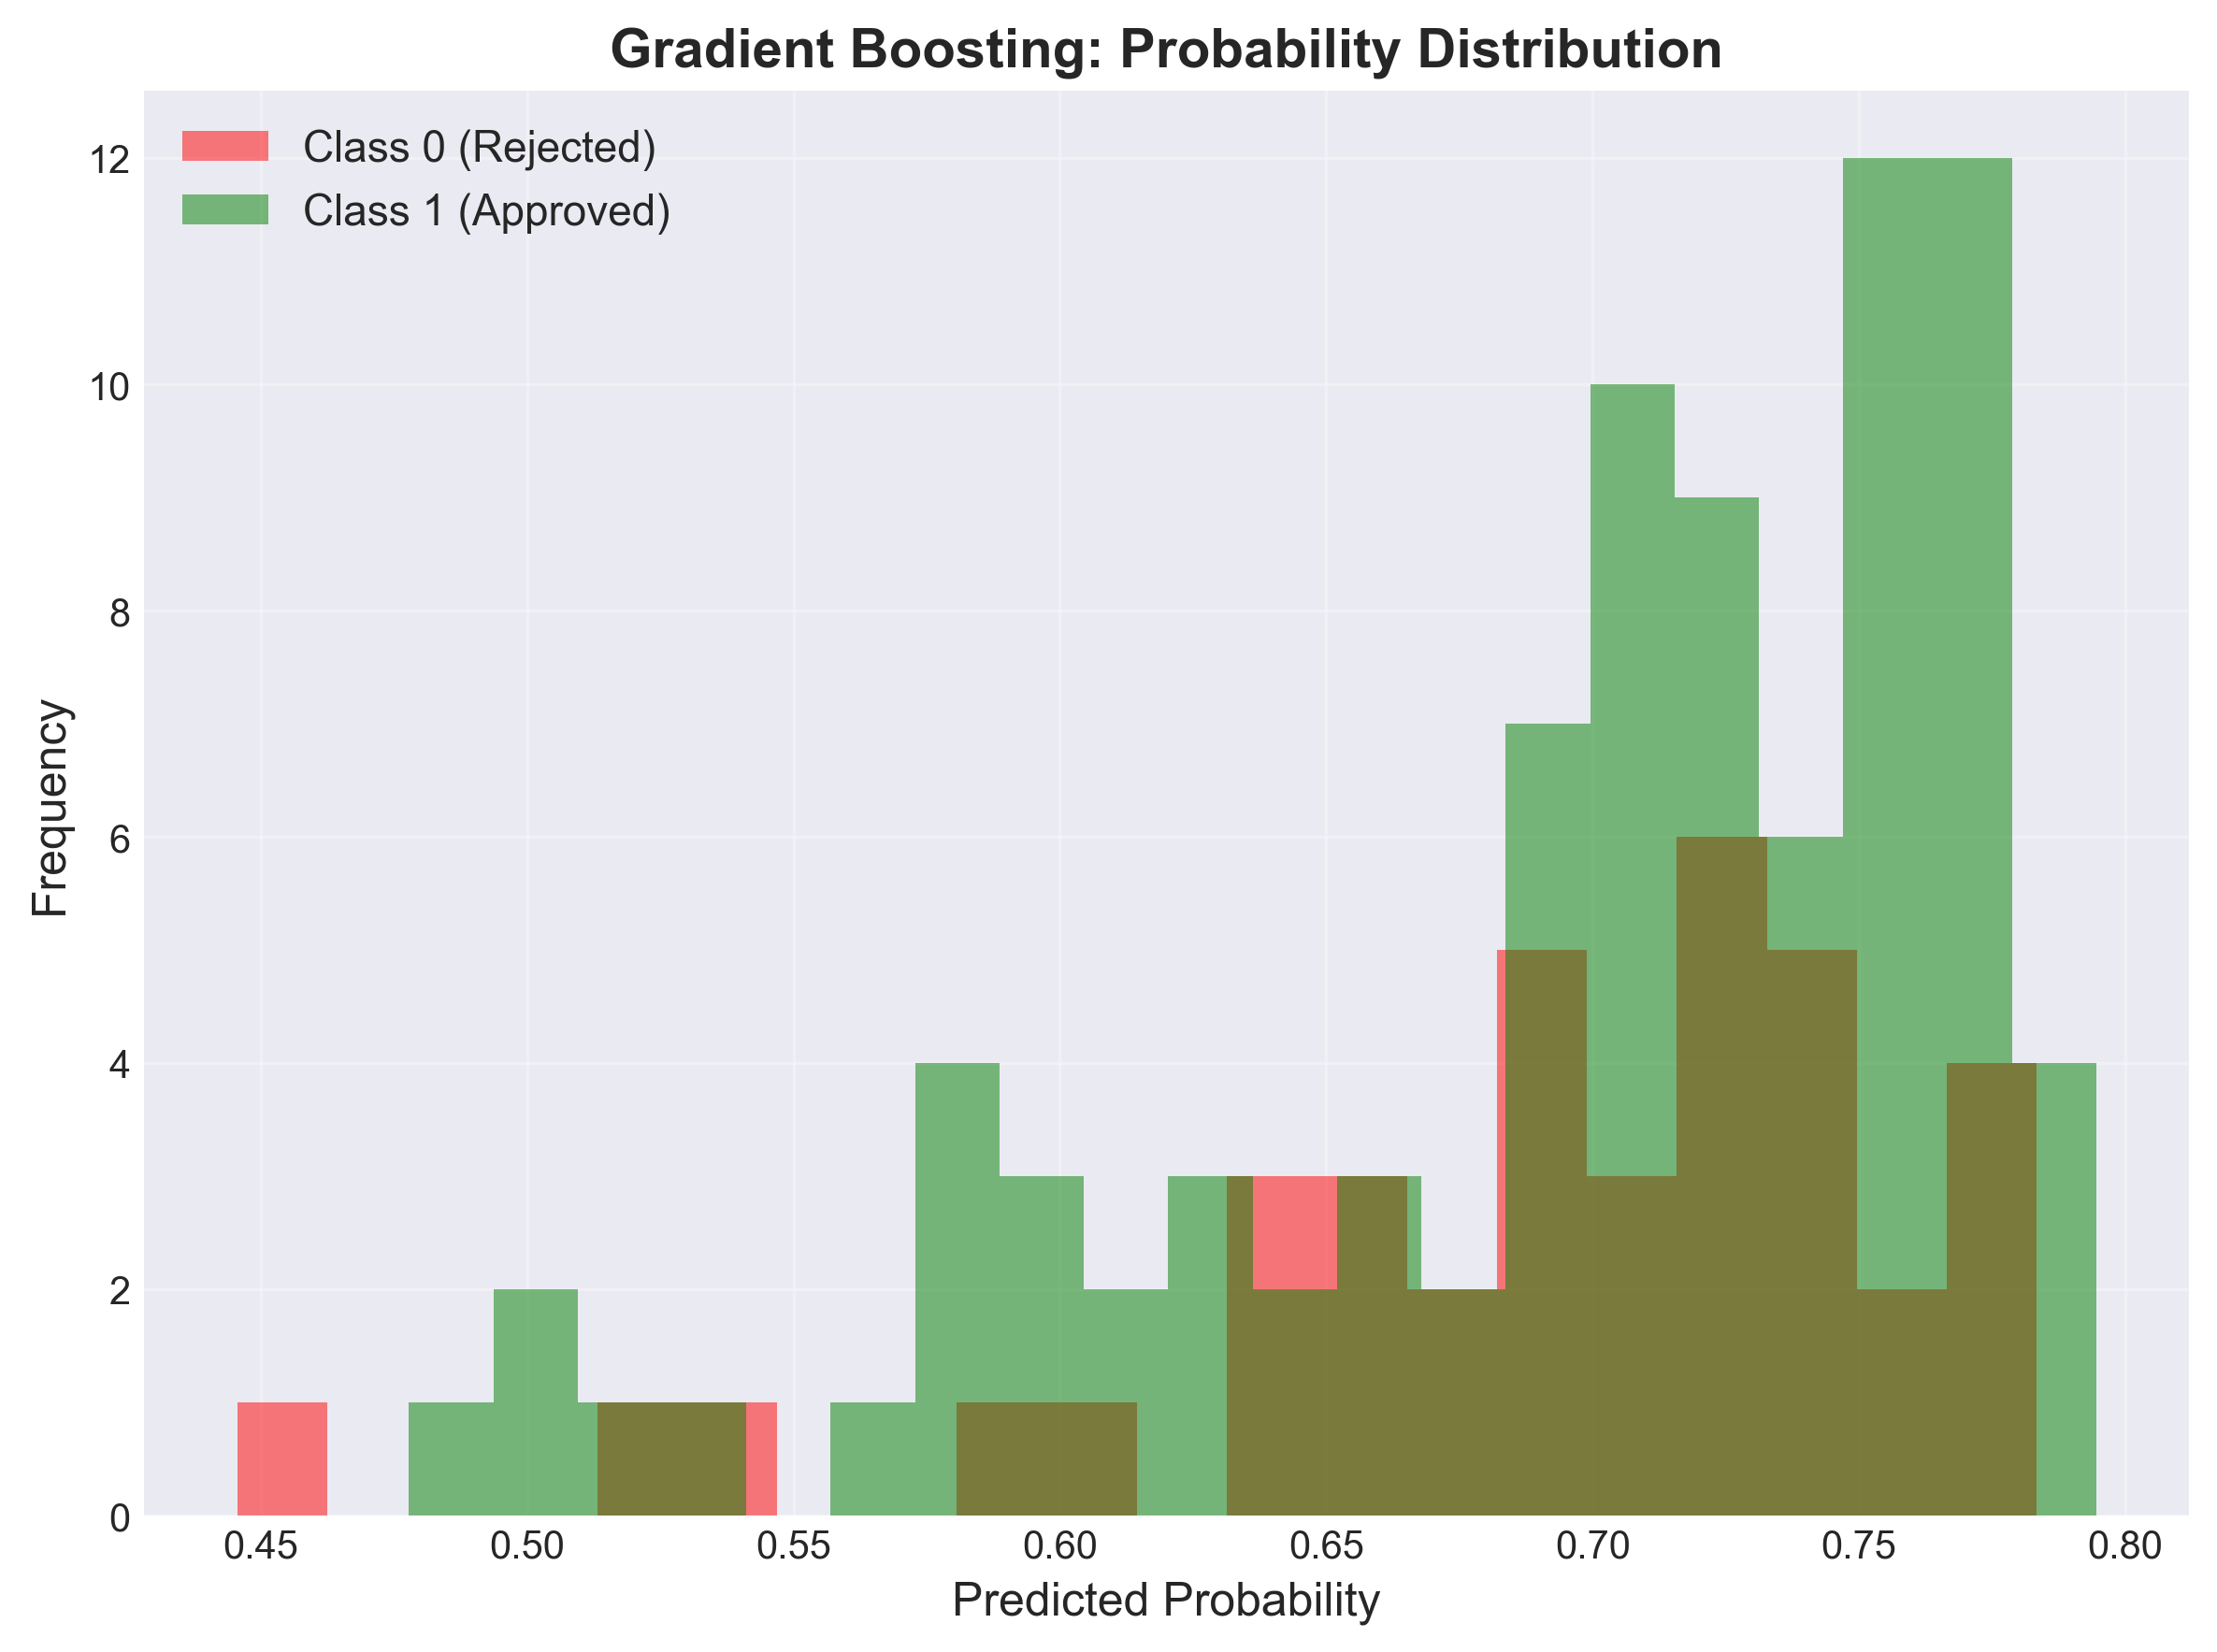
\includegraphics[width=0.7\textwidth]{img/probability_distribution_gb.png}
    \caption{توزیع احتمالات پیش‌بینی برای مدل Gradient Boosting}
    \label{fig:probability_distribution_gb}
\end{figure}

در شکل \ref{fig:probability_distribution_gb}، توزیع احتمالات برای مدل Gradient Boosting نمایش داده شده است. توزیع مشابه Random Forest است اما برای کلاس تأیید شده، تمرکز بیشتری در مقادیر بالاتر وجود دارد که با Recall بالاتر (\lr{96.47\%}) مطابقت دارد. برای کلاس رد شده، توزیع همچنان گسترده است که نشان می‌دهد مدل در شناسایی این کلاس مشکل دارد.

هر دو مدل اعتماد متوسطی به پیش‌بینی‌های خود دارند. مدل‌ها در شناسایی کلاس مثبت بهتر عمل می‌کنند اما در شناسایی کلاس منفی مشکل دارند. این می‌تواند به دلیل عدم تعادل کلاس یا قدرت پیش‌بینی پایین ویژگی‌ها باشد.

\subsubsection{خلاصه مقایسه مدل‌ها}

در این پروژه، \lr{Gradient Boosting} با F1-Score بالاتر (\lr{0.8039} در مقابل \lr{0.7872}) و Recall بالاتر (\lr{96.47\%}) عملکرد بهتری داشت که نشان می‌دهد این مدل در شناسایی وام‌های خوب عملکرد عالی دارد. همچنین، \lr{Random Forest} با استفاده از \lr{class\_weight='balanced'} به Precision بالاتری (\lr{71.84\%} در مقابل \lr{68.91\%}) دست یافت که برای سیستم وام بسیار مهم است چون باعث کاهش False Positive می‌شود. این نشان می‌دهد که انتخاب مدل بهینه به معیار ارزیابی مورد نظر بستگی دارد: اگر F1-Score و Recall مهم باشند، \lr{Gradient Boosting} بهتر است، اما اگر Precision مهم باشد (که برای سیستم وام اینطور است)، \lr{Random Forest} با \lr{class\_weight='balanced'} انتخاب بهتری است. هر دو مدل عملکرد قابل قبولی دارند و برای کاربردهای واقعی مناسب هستند. برای بهبود بیشتر، می‌توان از روش‌های پیشرفته‌تر مدیریت عدم تعادل کلاس مانند \lr{SMOTE} استفاده کرد، آستانه تصمیم‌گیری را تنظیم کرد، یا از ویژگی‌های مهندسی شده استفاده کرد.

\section{نتیجه‌گیری}\label{Section:Conclusion}

این پروژه شامل چهار بخش اصلی بود که هر کدام جنبه‌های مختلفی از یادگیری ماشین و یادگیری تقویتی را پوشش می‌دهند. در سوال \lr{۱}، انتخاب ویژگی با استفاده از الگوریتم‌های PSO و GA انجام شد و هر دو الگوریتم ویژگی \lr{Credit\_History} را به عنوان مهم‌ترین ویژگی انتخاب کردند که با دقت \lr{80.67\%} همراه بود. در سوال \lr{۲}، خوشه‌بندی داده‌ها با استفاده از سه الگوریتم مختلف انجام شد و \lr{DBSCAN} با امتیاز \lr{Silhouette} برابر \lr{0.5296} بهترین عملکرد را داشت. در سوال \lr{۳}، بررسی نظری الگوریتم یادگیری Q انجام شد و معادله، پارامترها و مسائل همگرایی مورد بررسی قرار گرفت. در پروژه نهایی، پیاده‌سازی کامل خط لوله یادگیری ماشین انجام شد و \lr{Gradient Boosting} با F1-Score برابر \lr{0.8039} بهترین عملکرد را داشت.

%\printbibliography[title=منابع]

\section*{منابع}

\renewcommand{\section}[2]{}%
\begin{thebibliography}{99}
\bibitem{b1} Scikit-learn Documentation: \href{https://scikit-learn.org/}{\lr{https://scikit-learn.org/}}
\begin{LTRitems}
\resetlatinfont
\bibitem{b2} PySwarms Documentation: \href{https://pyswarms.readthedocs.io/}{\lr{https://pyswarms.readthedocs.io/}}
\bibitem{b3} DEAP Documentation: \href{https://deap.readthedocs.io/}{\lr{https://deap.readthedocs.io/}}
\bibitem{b4} Sutton, R. S., \& Barto, A. G. (2018). Reinforcement learning: An introduction. MIT press.
\end{LTRitems}

\end{thebibliography}

\end{document}
